\documentclass[a4paper,twoside,openleft,12pt]{filipecorreiathesis} % define the title 
\usepackage[a4paper,margin=2.5cm, top=3cm, bottom=3cm]{geometry} % use bindingoffset=2cm for binding
\usepackage{appendix}
\usepackage{makeidx}
\usepackage{fancyhdr}
\usepackage{amsfonts, amssymb, amsthm, mathrsfs}
\usepackage{multicol}
\usepackage{multirow}
\usepackage{setspace} 
\usepackage{xspace}
\usepackage{algorithm, algorithmicx, algpseudocode}
\usepackage{rotating}
\usepackage{courier}
\usepackage{textcomp}
\usepackage{booktabs}
\usepackage{bookmark}
\usepackage[ISBN=555-555-555-555-0,SC0]{ean13isbn}
\usepackage{wrapfig}
\usepackage{soul} % provides yellow-marker highlighting among other features
\usepackage{verbatim} % provides the 'comment' environment among other features
\usepackage{xifthen} % provides \ifthenelse 
\usepackage{multirow}
\usepackage{enumitem}
\usepackage{pbox}
\usepackage[section]{placeins} % stops floats (figures, tables...) to appear outside the section where they are placed.
\usepackage{cleveref}[2012/02/15]

\usepackage{longtable}
\usepackage{subcaption}

\usepackage{calligra}
\newcommand{\setfont}[2]{{\fontfamily{#1}\selectfont #2}}

% \usepackage[disable]{todonotes}
\usepackage[]{todonotes}
\presetkeys%
    {todonotes}%
    {inline,backgroundcolor=yellow}{}

\makeindex

% dividing diamonds
\newcommand{\dividingdiamonds}{\vspace{0.2cm}\centerline{$\diamond \diamond \diamond$}\vspace{0.2cm}}%


%\onehalfspacing
\setstretch{1.3} % for custom spacing

% indentation of multiline figure/table captions.
%\usepackage[format=plain,justification=RaggedRight]{caption}

% Vertically centered table columns
\newcolumntype{M}{>{\centering\arraybackslash}m{\dimexpr.25\linewidth-2\tabcolsep}}

%% Fixes problem with bibliograpy key protruding into description
\usepackage{eqparbox}
\usepackage[numbers]{natbib}
\renewcommand*{\bibnumfmt}[1]{\eqparbox[t]{bblnm}{[\textcolor{feup}{#1}]}}

\def\isnum#1{%
  \if!\ifnum9<1#1!\else_\fi
    \oldstylenums{#1}\else#1\fi}

%% Fancy Headers -- Somehow, I can't seem to be able to move this to the .cls file
\pagestyle{fancy}
\fancyhf{}
\fancyhead[LE]{\small \leavevmode\llap{\textcolor{feup}{\isnum{\thepage}}\hspace{0.5cm}}\smallcaps{\leftmark}}
\fancyhead[RO]{\small \leavevmode\smallcaps{\rightmark}\rlap{\hspace{0.5cm}\textcolor{feup}{\isnum{\thepage}}}}
\fancypagestyle{plain} {
 \fancyhf{} % get rid of headers on plain pages
 \renewcommand{\headrulewidth}{0pt} % and the line
 \renewcommand{\footrulewidth}{0pt} % and the line
}
\renewcommand{\headrulewidth}{0pt}
\renewcommand{\footrulewidth}{0pt}
\setlength\headsep{1.1cm}
\setlength\headheight{13.6pt}

\renewcommand{\chaptermark}[1]{\markboth{#1}{}}
\renewcommand{\sectionmark}[1]{\markright{#1}{}}

%% Define a new 'leo' style for the package that will use a smaller font.
\usepackage{url}
\makeatletter
\def\url@leostyle{%
  \@ifundefined{selectfont}{\def\UrlFont{\sf}}{\def\UrlFont{\footnotesize\ttfamily}}}
\makeatother
\urlstyle{leo}

%\usepackage{inconsolata} % monospace font, used for \texttt{}


\begin{document}
	\title{TESThesis }
	\author{\href{mailto:your-email-address@fe.up.pt}{Pedro Miguel Lourenço Costa}}

	\frontmatter
	    \pagestyle{empty}
	    \maketitle
		\noindent\textbf{Contact Information:} \\

\noindent Pedro Miguel Lourenço Costa \\
Faculdade de Engenharia da Universidade do Porto \\
Departamento de Engenharia Informática \\

\noindent Rua Dr. Roberto Frias, s/n \\
4200-465 Porto \\
Portugal \\

\noindent Tel.: +351 968 203 386 \\
Email: pedro.miguel.costa@fe.up.pt \\
URL: https://www.linkedin.com/in/pedro-costa-3279996b \\

\vfill


		\cleardoublepage
		\begin{flushright} 
  %\null\vspace{\stretch{1}}
  \null
  \vfill
  \emph{\Large{\dots to the world in general}} \\
  \vspace{3cm}
\end{flushright}
		\clearpage
		{\centering \emph{This page was intentionally left blank.} \\ }
		\cleardoublepage
		\pagenumbering{roman}
		\pagestyle{fancy}
		\chapter{Abstract}


Nowadays, nearly every medium-size or large company in the electronics, pharmaceutics, food, or other industries needs to support its operations by managing the exchanged information and resources. The upstream and downstream flow of these, together with the system of organizations, people and activities that make it possible, is commonly referred to as a supply chain. In a practical sense, a supply chain’s flow of products and services goes from supplier to consumer. For example, the supermarket fish a person eats: it is caught in boats, then prepared, and distributed to a store where the final consumer is able to buy it. But supply chains are becoming very complicated and complex systems, spanning multiple businesses and relationships, interlaced in many different ways, which is a reason why supply chain management (SCM), the discipline which deals with the coordination of a supply chain, is becoming increasingly more important.  The information has to flow through the chain, sometimes even reverting the direction, but the paths it takes are not always very obvious or even traceable in the global context, dealing with many issues along the way.

Managing inventory and suppliers while maintaining safety, quality and keeping to the schedule is a difficult task. Delays are common, and a company’s finances, growth and reputation are affected. This is further aggravated by the fact that information is not always accurate or available when needed. And the fact that companies value their privacy makes it so that sharing information with others is not always simple or desirable. 

Most important of all, frequently, there are big holes of information in a supply chain, analog gaps where the information has not been made digital in the system. The use of traditional tools is still too prevalent. Emails are sent, documents are printed and mailed, instead of making the information digital, putting  it directly on the network and relaying it to the next link in the chain. This fact, together with the sometimes apparent lack of interoperability between the SCM software of different companies and their need to protect their private information is what makes a global overview of the whole chain complicated with the current technologies. Provenance and traceability of a supply chain are a big objective for companies, along with improving security, efficiency and effectiveness of the supply chains.

Most of these issues are, in great part, caused by the standalone use of outdated or inadequate software architectures, which, traditionally, are often centralized and have single points of failure. And even when they are not, oftentimes they are insecure, prone to synchronization problems, leading to big delays in both relaying the information and resources and making payments possible. 

One way to approach these specific problems of supply chains that are brought by the traditional IT solutions is to update them with new infrastructures, namely by using blockchain technology. Blockchain is a decentralized technology that has no single point of failure and allows for the immutable storage of verifiable data all over the computers that store it. Each time there is a new piece of information, its validity is verified by the network and it is inserted into a block of the chain, which leads it to being continually extended. This means that we can check all the information that there ever was, since the beginning, and validate it easily, or make any necessary calculations. As such, blockchains are the perfect means to achieve traceability of a supply chain. At the same time they are a secure and incorruptible way to store information, with a fast synchronization time, being perpetually available to anyone, anywhere within the network. It would also be the way to close the analog gaps, turning the chain fully digital, leading to the possibility of a global overview.

This project focuses on researching the effects of applying blockchain technology to a supply chain and its management. By doing this, it should be possible to ascertain how much this technology can really impact SCM over the traditional IT solutions, or in combination with them. A practical instance involving the application of this technology to a system will also be developed, to further demonstrate its possible benefits.

The improvements that it could bring are, however, not limited to the problems described. Blockchain is a whole new game, and it brings a whole new myriad of possibilities into the table. We are only seeing the tip of the iceberg and this is an area that is of the interest of any company which aims to improve the efficiency and effectiveness of its entire supply chain system.

\textbf{Keywords:} Supply Chain, Supply Chain Management, Industry, Blockchain, Network, Decentralization, Security, Traceability, Provenance, Information Integration, Ledger, Interoperability


\chapter{Resumo}

Tradução PT do abstract





		\addtocontents{toc}{\protect{\pdfbookmark[0]{\contentsname}{toc}}}
		\tableofcontents
		\cleardoublepage
		\phantomsection
		\addcontentsline{toc}{chapter}{\listfigurename}
		\listoffigures
		\cleardoublepage
		\phantomsection
		\addcontentsline{toc}{chapter}{\listtablename}
		\listoftables
		\cleardoublepage
		%\chapter{Preface}

\epigraph{\emph{
A quote
}}{\sc The Quote's Author}
\vspace{1pc}


Lorem ipsum



	\mainmatter

	\todo{pedro: compor captions das tabelas, por em cima e com nome correto}
	\todo{pedro: compor tamanhos das tabelas}
	\todo{pedro: por so 2 casas decimais nas tabelas}
	\todo{pedro: compor imagens dos graficos}
	\todo{pedro: consistent with the use of bold or italic, especially on thesis questions}
	\todo{pedro: corrigir localizacoes das figuras}
	\todo{pedro: captions das questions na survey, compor para terem QUESTION}
	\todo{pedro: introducao + structure}
	\todo{pedro: abstract precisa de ser revisto de maneira a sumariar bem todo o conteúdo da tese}

	%\subsection*{2. Naming Conventions and Definitions}
	%glossary ->    \todo{fcorreia: isto devia aparecer talvez no início do documento, num glossário geral}

	%	\par PoC - Proof of Concept
	%	\par SLA - Service Level Agreement
	%	\par Other glossary terms, acronyms and whatever.
		
     %   \subsection*{3. Relevant Facts and Assumptions}
	%	\par N/A - Random stuff that is not put anywhere else, basically

	% final lineup
    %\chapter{Introduction1}
%\minitoc \mtcskip \noindent
%\chapter{Introduction2}
%\minitoc \mtcskip \noindent
\chapter{Introduction}
\label{chap:introduction}
\minitoc \mtcskip \noindent

Our society is turning more consumerist, with most people in developed countries having high consumer power and standards of life. Consumers goods, from the essentials up until the entertainment goods, are manufactured and ordered continuously in high quantities.

Modern supply chains feel the pressure of this growth, leading to the demand for an efficient management. Most companies are making efforts towards this end, and, even though part of the answer to an efficient management lies in having efficient processes, a good management is also based in using the right technologies. Thus, the development of technologies that can satisfy the demands of supply chain management, for any industry, is in high demand.

%The development of such technologies should be faced towards the problems that supply chains 

%ace concerns are raised as to whether the demand can be met in a transparent and trustful way. It is difficult to know where the products we consume come from, and the processes they go through. This leads to the need of transparency in the supply chains as well as the need of an increase in their efficiency, if they are to conform to the market's needs.

\section{Supply Chains}
\label{supply_chains}
\textbf{Supply Chains} can be found, in some form, in nearly every business, spanning many different areas of operation. Traditionally, a supply chain encompasses all the processes and activities that lead from the initial raw materials to the final finished product, as well as all the functions and services within and outside a company. A supply chain can also be defined as the network of entities through which material flows. These entities can be identified as suppliers, carriers, manufacturing sites, distribution centers, retailers, and customers~\cite{Lummus2014}. Naturally, with the upstream and downstream flow of these materials and resources, comes a lot of information on them and on the processes, people and organizations they are associated with. Realistically, the  flow is not always arborescent, as there are many considerations to be taken and decisions to be made. Supply chains have multiple end products with shared components, facilities and capacities~\cite{Ganeshan1995}. As a consequence, the paths taken by the resources and information are not straightforward, but interlace, diverge and converge at different points, go back and forth, as exemplified in Figure~\ref{fig:supplychain_complexity}.
  
\begin{figure}[ht]
\centering
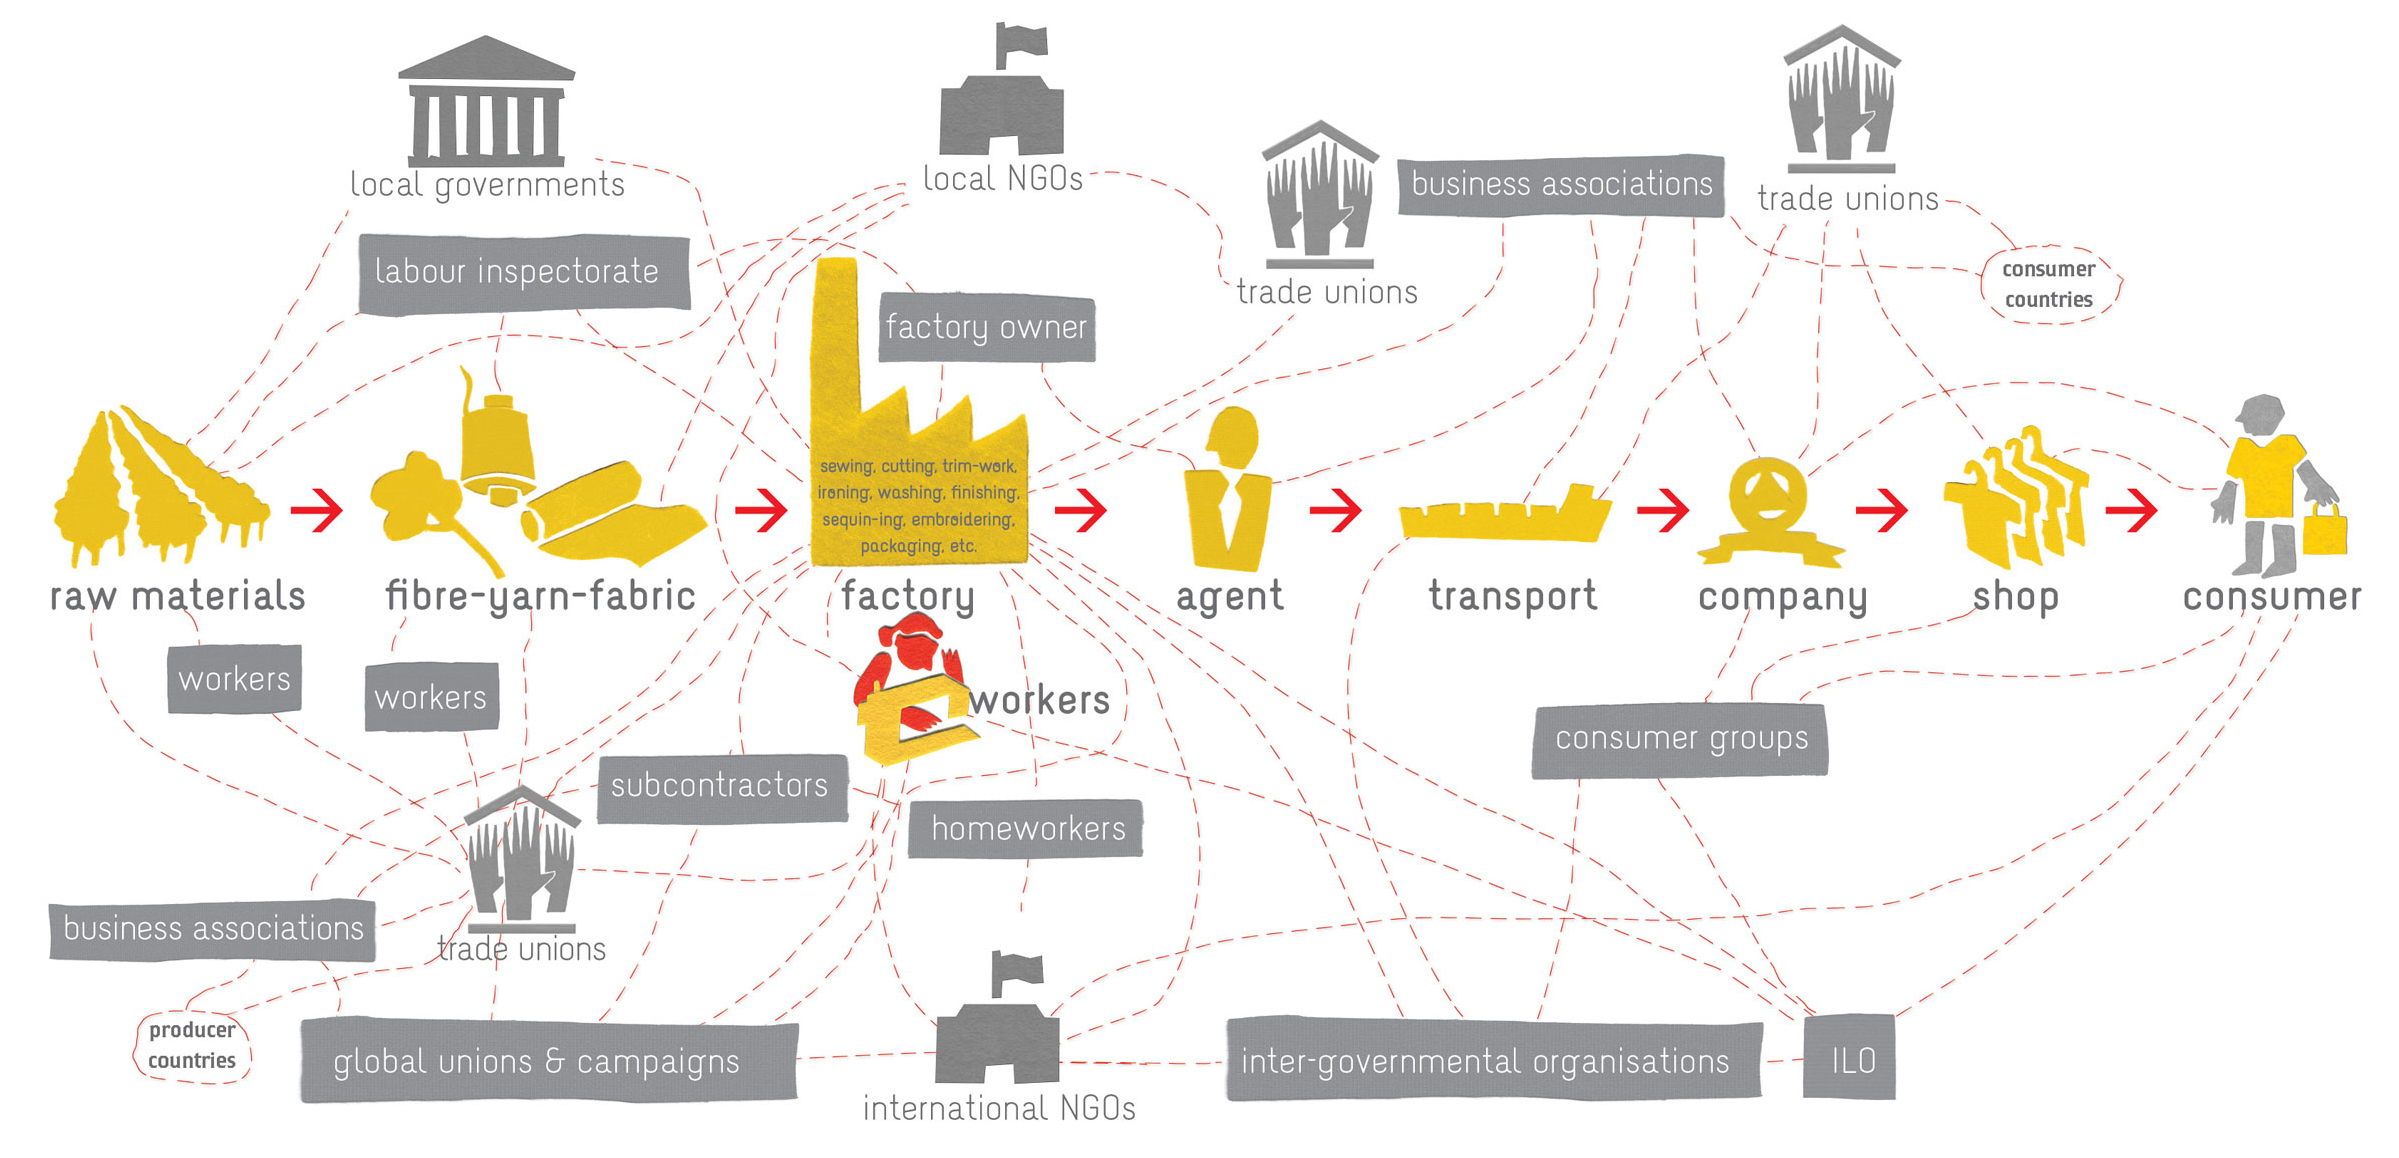
\includegraphics[scale=0.18]{media/supplychain_complexity.jpg}
\caption[Representation of a garment supply chain and all the relationships it involves]{Representation of a garment supply chain and all the relationships it involves. Taken from the International Training Centre of the International Labour Organization briefing on global supply chains~\cite{ITCILO2018}.}
\label{fig:supplychain_complexity}
\end{figure}
  
  The activities and processes a supply chain encompasses include: sourcing raw materials and parts, manufacturing and assembly, warehousing and inventory tracking, order entry and order management, distribution across all channels, delivery to the customer, and managing the information systems necessary to monitor all of these activities. As Lummus~\cite{Lummus2014} describes, these activities can be roughly mapped to the 4 essential processes: plan, source, make, deliver.
    
  Coordinating all of these is no easy task, and so the discipline of SCM comes into life. According to Ballou~\cite{Ballou2007}, the Council of SCM Professionals (CSCMP) defines SCM as \textit{“the planning and management of all activities involved in sourcing and procurement, conversion, and all Logistics Management activities. Importantly, it also includes coordination and collaboration with channel partners, which can be suppliers, intermediaries, third-party service providers, and customers. In essence, SCM integrates supply and demand management within and across companies”}.

From this definition follows that SCM deals a lot with both coordination and collaboration between entities, and so, the management of the flow of information and resources between them is very important. The objective is always, of course, to minimize the total cost of these flows between and among stages~\cite{Habib2011}.
In the end, the creation of value (products and services) in a supply chain stems from the relationships that different entities build between themselves, and not from the work of a single entity. As such, supply chains, not firms, compete and those which have the best integration and management processes win.

And this is where SCM shines and shows just how useful it can be. Managing all the processes in a supply chain, while maintaining safety, quality and keeping to schedule is difficult. An event on one side of the world, large or small, be it from human or natural causes, can easily disrupt the links in the supply chain. For instance, it might disrupt the supply of a critical component or service. Delays are, therefore, common, and the consequences of such disruptions might have a severe impact in the finances, growth and reputation of the companies involved~\cite{Punter2013}.

SCM diminishes the impact of such disruptions, and actively works to avoid or diminish them, while optimizing the way the supply chain works. This is why SCM is such an important discipline, that we have to better understand and improve, with all the means that we can, and this includes, of course, research into technologies like the blockchain.

\section{Challenges}
\label{sec:supply-chain-challenges}

 Having already introduced the concepts of Supply Chain and SCM, it is now possible to briefly introduce some of the problems that affect them.

The first, and most generalist problem of a supply chain, is the ease with which \textbf{an unexpected event might cause delays}. These events, already mentioned in Section~\ref{supply_chains} are not always predictable and must be contained as fast as possible. One event in particular which, often, causes delays are \textbf{synchronization problems in the processes and information systems of a company}~\cite{Prokle2017}. 

    Another problem is that, often, there are difficulties in sharing information between companies. This is caused both by the fact that \textbf{companies value their privacy and the security of their information}, which means they might not want to share too much information, or that they might only share it through secure channels, and by the \textbf{lack of standards for sending information and communicating}~\cite{Korpela2017}. The issue with non-existing standards is that companies are left to discuss what details to share or not, wasting time and resources.

Most important of all, in the industry, \textbf{the use of traditional tools and manual work is still too prevalent}. Emails are sent, documents are printed and mailed, instead of transmitting the information in a more automatic, direct and secure way through the network. This point also brings the next problem of supply chains to light: the apparent lack of interoperability between certain softwares (which might be a byproduct of by the lack of standards).
 
 
Finally, provenance and traceability of the products on a supply chain are a big objective for companies. But \textbf{the current technologies used in supply chain only accomplish provenance and traceability in a limited scope}, as the information a certain entity possesses is usually also limited. And so, it is very hard for anyone to have a global overview of the supply chain.

Though it is not proven, it is be possible that some, if not most, of these issues in supply chain might be caused by the use of software architectures that do not allow for full data integration. An optimal supply chain should be as efficient and effective as possible, while being secure and satisfying all the traceability requirements. Perhaps, it is time to try out new solutions which replace or augment the existing ones, in such a way that supply chain management can better satisfy the needed requirements.

\section{From Blockchain Technologies to Supply Chains} \label{sec:context}

Blockchain technology allows for secure, public, distributed and decentralized systems. Though it was first proposed in its actual form by Satoshi Nakamoto~\cite{Nakamoto2008}, an anonymous group which published a white paper in 2008, this was not the first reference to such a technology. The first work on a cryptographically secured chain of blocks was described in 1991 by Stuart Haber and W. Scott Stornetta~\cite{Haber1991}, and further refined in 1992 by Bayer \& Haber, by incorporating Merkle trees~\cite{Bayer1993}. Since then, it has come a long way, sprouting multiple different uses and applications of the technology. Its characteristics make the development of distributed and permanently, globally available systems possible, which is a paradigm that is attracting the interest of various industries.

One area in particular where we believe blockchain could bring about great improvements is Supply Chain Management (SCM). SCM has seen an increase in complexity in the last few decades, due to the globalization of the market, with businesses interlacing in many different ways, their relations extending way beyond what they used to, as found by Filiz Isik~\cite{Isik2011}. This increase in complexity is somewhat hard to manage and some supply chains stretch and encompass so many businesses that, due to their software not being prepared for this, the information is not always transmitted from end to end, leaving holes of information in between the links that join each business, thus leading to a lot of chaos and uncertainty as to the state of the key items in the chain~\cite{Wilding1998}.

   This dissertation work will focus on supply chain management, and on how blockchains can possibly be applied to improve this area, leading to positive impacts in the logistics industry and eventually finding benefits for the consumer as well. 

%%%%%%%%%%%%%%%%%%%%%%%%%%%%%%%%%%%%%%%%%%%%%%%%%%%%%%%%%%%%%%%%%%%

\section{Motivation} 
\label{sec:motivation}

As described in section~\ref{sec:supply-chain-challenges}, a possible cause of these problems might be the use of software that can not keep up with the evolution of the requirements of modern supply chains. Today's supply chains have high standards for their requirements and even when the software works just fine, maybe it is not recent enough or it was not specified and built to satisfy these requirements. For instance, product falsification might be a huge issue nowadays in the supply chain, but maybe it was not rated as a high importance problem 15 years ago. Therefore, the software from 15 years ago complied with different requirements than the ones from today and was not built to handle that specific problem well. 

\textbf{Requirements evolve, and so should the technology, in order to support them.} There is an immediate need for solutions, which might either completely replace the previous ones, or augment them.

One way to approach these specific problems is to research what would a modern requirements specification for supply chain look like, and develop new technologies that are more accurately specified for the supply problem challenges in question. 

The characteristics of blockchain architectures seem to be a good solution for many of the identified problems in supply chain to be reduced or neutralized. These architectures are the perfect means to achieve traceability of a supply chain, and so, they are good to achieve provenance as well. At the same time they are a secure, incorruptible and immutable way to store information, with a fast synchronization time, being perpetually available to anyone who has permission, anywhere within the network. It would also be the way to close the analog gaps, turning the chain fully digital, leading to the possibility of a global overview.

\section{Objectives}
\label{sec:objectives}
The main objective of this dissertation is to find whether blockchain technology is a good fit to solve the most common problems of supply chain management, and also to find out the technological requirements of a modern supply chain. There are a multitude of small tasks that blockchain could automatize in supply chain, so this thesis will try to figure out which ones blockchain applies to better. 

The primary objective of this dissertation is determining if blockchain architectures can be successfully applied to supply chain management as an improvement towards the technologies that are already being used. For this purpose, it is necessary to conduct research on the supply chain issues and validate these, in order to propose a blockchain design that can target these issues successfully. 

\section{Dissertation Structure} \label{sec:struct}

Besides the introduction, this dissertation has 6 more chapters, divided into 2 parts.

\par \textbf{Part 1: Background and State of the Art} - Provides the needed concepts to understanding the work, as well as explanations about the existing tools and projects related to the blockchain and to its application to supply chain management domain.
 The state of the art is divided into 2 chapters:~\ref{chap:blockchain} and ~\ref{chap:blockchain-applicability}.
\begin{itemize}
  \item Chapter~\ref{chap:blockchain}, "Blockchain Technologies", some important concepts from the blockchain architecture are presented and discussed, followed by an analysis of the existing blockchain networks and frameworks and their comparison.
  \item Chapter~\ref{chap:blockchain-applicability}, "Blockchain in the Industry", the application of blockchain to supply chain is discussed in more detail, including the possible advantages, challenges, and following it up with an analysis of the existing blockchain applications that also focus on supply chain. 
\end{itemize}

\par \textbf{Part 2: Problem, Research and Solution} - Provides a thorough explanation of the problem, objectives and the proposed methodology to approach them. Follows up with a survey and requirements analysis, which serves as a base to propose a blockchain solution design. 
\begin{itemize}
  \item Chapter~\ref{chap:supply-chain-problems}, "Problem Statement", specifies the thesis statement and the questions that need to be answered in order to reach a conclusion.
  \item Chapter~\ref{chap:survey}, "Supply Chain Issues Validation and Requirements Elicitation", features a survey and the analysis of its results, such as to gather the requirements for a supply chain system, so that a blockchain-based solution can be proposed.
  \item Chapter~\ref{chap:prototype}, "Solution Design and Implementation", features the choice of a blockchain framework and the proposal of a solution, which consists in building a proof of concept (PoC) project that implements the requirements elicited from the survey.
\end{itemize}

\par \textbf{Part 3: Conclusion} - Gathers all the information from the results of the solution to make a statement, also listing contributions, difficulties and future work.
\begin{itemize}
  \item Chapter~\ref{chap:conclusions}, "Conclusions", features an overview of the work done in the dissertation, providing an answer to the previously defined problem, and following it up with possibilities of future work in this area.
\end{itemize}
    \chapter{Blockchain}
\label{chap:blockchain}

\minitoc \mtcskip \noindent

This chapter introduces the most important concepts of blockchain which are essential for its applications. It interleaves the features of blockchain with its applicability to supply chain, by highlighting both the disadvantages and disadvantages, of blockchain in general and in particular to SCM, as well as any existing models for the integration of blockchain with SCM.

\section{Introduction}
“The Byzantine Generals' Problem” is a classical problem faced by distributed systems, which, in simple terms, states that consistency in a distributed system can never be fully guaranteed \cite{byzantine-generals-problem}. This is derived from a lack of general consensus as to what the state of the system is at any given time.

Nakamoto's implementation of a blockchain seems to be, at present, the most practical way to approach this problem (though with its limitations), even earning the term "Practical Byzantine Fault Tolerance (PBFT) Algorithm", because of how it handles the consensus issue. The fact that many kinds of applications rely on distributed architectures, which might face these problems, turns blockchain all the more appealing. 
   
Some improvements have been built upon the traditional blockchain, such as smart contracts, which further enhance its use and allow for a wider variety of applications. Some areas where blockchain is starting to see some use include insurance, finance, Internet-of-Things, health care, identity management, to name a few.

In each of these areas, there are many ways in which blockchain can be used, be it to store information, process information, process payments or provide services. The versatility is what makes it so popular and what allows for the possibility of many other applications to be proposed.

\section{Core Concepts and Features}

%\paragraph{Original blockchain}    
The original blockchain, Bitcoin, was developed with the purpose of creating a distributed online payment system without the need for a financial institution or any other centralized trusted third party to verify the transactions. It even has its own currency, made up from digital tokens that represent real money, a concept which is now commonly known as a cryptocurrency.

Eventually, this concept evolved into something more, and new uses, other than online transactions, emerged from the blockchain technology. As described by Marc Pilkington \cite{Pilkington2015}, \textit{"the essence of the blockchain is informational before being economic or monetary, conducive to many emerging and increasingly popular token-free blockchains."}

Therefore, the algorithms used by Bitcoin are not a defining feature of the blockchain technology, but merely one of the many possible applications.
    
    The blockchain itself consists of a peer-to-peer network which continually stores and updates a chronological chain of blocks, where each block stores whatever information is relevant to the system in question, as well as the hash of the previous block. In the original blockchain, each block stored information about transactions between people, where there was a set of rules to check whether the transactions were valid or not. We'll get to how a blockchain can be built in a moment.
    
    One important and defining property of the blockchain is that the hash of the previous block also serves as an address. Therefore, each block has a pointer to the previous block, which is known as an hash pointer. This concept is illustrated in Figure \ref{fig:blockchain_workflow}.
    
\begin{figure}[h]
\centering
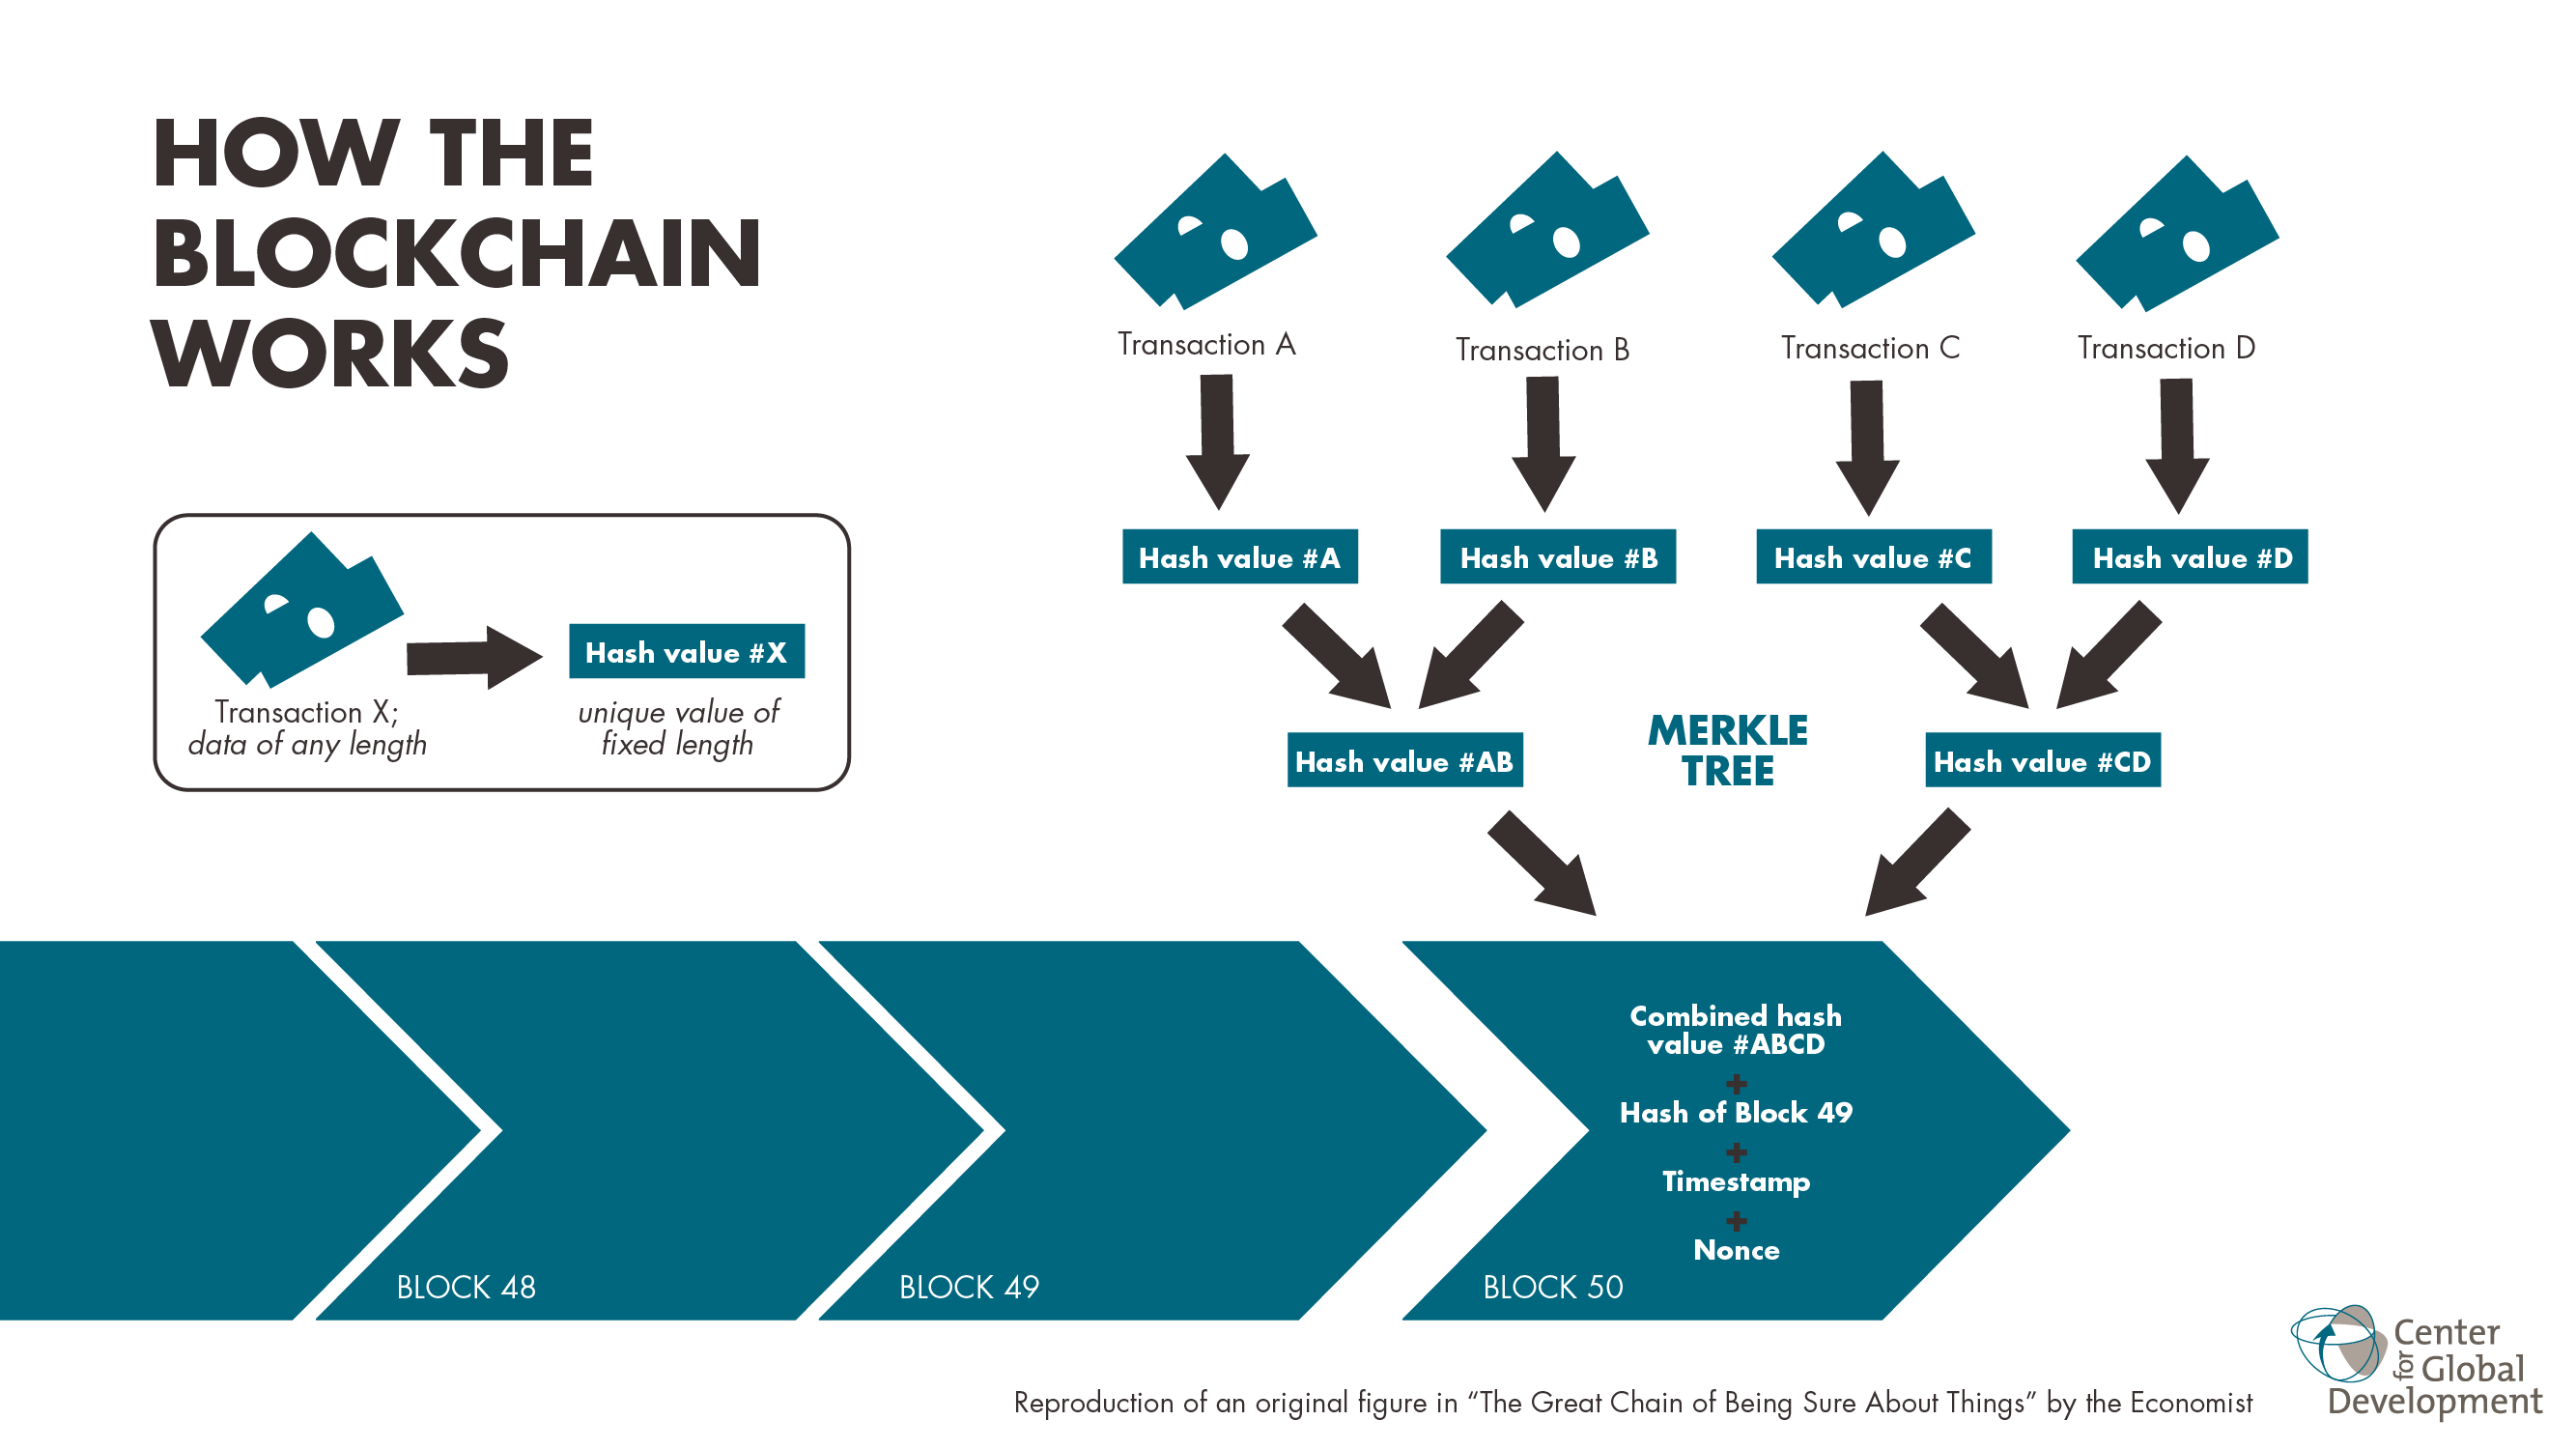
\includegraphics[scale=0.35]{media/Blockchain_workflow.png}
\caption{Representation of a blockchain's structure}
\label{fig:blockchain_workflow}
\end{figure}

\subsection{Immutability}
    This hash thus guarantees that the blocks are linked to each other, but it also guarantees the integrity of the block chain. If one block is altered, the hash on the block that follows it stops matching the block's. If we really wanted to change something on this  first block, we would have to alter the hash on the following block to match. But then, that second block would also have been altered, and we would have to change the hash on the third block to match, and so on. This means that the blockchain is immutable, as it is not possible to alter a single block without manually altering all the others. 
    
\subsection{Consensus}
    The blockchain and its data exists only in a \textbf{peer-to-peer network}, and as such, it is stored and extended by the nodes of the network, which form a topology between them. The nodes are machines that have the core code of the blockchain system and which receive and share among themselves the incoming information, in the form of blocks, validating it according to the established rule set. All the nodes, if they are not malicious and actively attempting to change the contents of the chain, contain the same blockchain structure and information, as they all agree on its contents through a consensus algorithm. 
    
     Some nodes are open to the internet and the world, thus receiving information from outside the peer-to-peer network and disseminating it to the rest of the network's nodes. A subset of the nodes, called miners, will then gather the circulating information from the peer-to-peer network (by receiving transactions from the nodes they are connected to), and form blocks of information, which they try adding to the blockchain. Obviously, it is impossible for all the nodes to add their blocks at the same time, as each of them would then have a different version of the blockchain and they would get desynchronized. And so, the nodes must reach a consensus as to which block gets added next to the blockchain. For this very reason, the code of the blockchain must have both a consensus algorithm and also a block validation algorithm.
     
     In public blockchains, the mining nodes do all the hard work, and they usually need some incentive to do so. Cryptocurrencies are virtual currencies that only exist on the blockchain they belong to, and they allow for a new monetary system to come into life. These currencies play an important role in blockchain, since they allow for miners to be rewarded. Without them, public blockchains would probably not work as well, which is why there are so many alternative currencies popping up, with the advent of this technology. 
     
     Of course, this is just one of many ways to make a blockchain move forward successfully, and other types of consensus algorithms have been idealized, though most of the consensus algorithms in public blockchains will use cryptocurrencies as the prime incentive.
    
    
\subsection{Private, Public and Hybrid Blockchains}

    Blockchain, traditionally, is of public nature. But, as many institutions grew aware of the possible benefits of this technology, they started investing in it, and so appeared the private blockchains and the semi-private or consortium blockchains.
    
    \paragraph{Public Blockchains} When a blockchain is public, it is accessible to any user. Anyone is able to both read and validate information from it, as well as contribute to its extension by participating in the consensus process. They are secured by the economic incentives that are given to the miners, in the form of cryptocurrency tokens. These blockchains can be  considered fully decentralized and have no access control. Every user is at the same level.
    
    \paragraph{Private Blockchains} These are usually owned by some organization and have access control, restricting write access to certain peers inside the organization. Read access might be restricted or not, according to the organization's goals. These blockchains, unlike public ones, might not require cryptocurrency or incentives, as the maintenance of the blockchain is done by the organization who owns it, and so they have all the interest in having nodes that can run the consensus process. In the end, this is a more centralized version of the blockchain, as the nodes are concentrated under the ownership of the organization. This also gives the advantage that alterations to the blockchain are easier to achieve, if so is desired (though it subtracts from the actual meaning and concept of an immutable blockchain). It is usually more efficient than public blockchains, being able of achieving a higher number of transactions processed per second.
    
    \paragraph{Consortium blockchains} They are a kind of hybrid blockchain, though closer to a private blockchain. They are controlled by many different organizations, and the consensus process is handled by pre-selected nodes from the organizations. This consensus might involve, for example, at least a certain percentage of the nodes agreeing on something (e.g.: if there are 15 fixed nodes, require at least 10 to sign the block). The permissions to read might be public or otherwise permissioned, and as such, this can also be considered a partially decentralized blockchain.
    % TODO: INCLUDE QUOTE
   % “So far there has been little emphasis on the distinction between consortium blockchains and fully private blockchains, although it is important: the former provides a hybrid between the ‘low-trust’ provided by public blockchains and the ‘single highly-trusted entity’ model of private blockchains, whereas the latter can be more accurately described as a traditional centralized system with a degree of cryptographic auditability attached.”[2] 

%--> Hyperledger composer leans more towards the consortium permissioned blockchain type
    \subsection{Types of Consensus Mechanisms and Algorithms}
    
     The most commonly used consensus algorithm is \textbf{Proof of Work (PoW)}, though there are others, like the most used alternatives, \textbf{Proof of Stake (PoS)}, and \textbf{Proof of Activity (PoA)}. We showcase some of the algorithms in table %TODO: PUT REFERENCE 2.1.
    
%%%%%%%%%%% TABLE

%TODO: FIX THIS

% Please add the following required packages to your document preamble:
% \usepackage[normalem]{ulem}
% \useunder{\uline}{\ul}{}
\begin{table}[]
\centering
\caption{My caption}
\label{my-label}
\begin{tabular}{|l|l|l|}
\hline
Type                                                                       & Overview                                                                                                                                                                                                                                                                                                                                                                                                                                                                                                                                                                                                     & Better Used In                                                                           \\ \hline
Proof of Work (PoW)                                                        & \begin{tabular}[c]{@{}l@{}}In short, PoW works by making the nodes spend \\ computational power until they can find out a hash \\ that satisfies a certain rule, for a certain block. When \\ a node finds this hash, it is allowed to extend the \\ blockchain with that block. The node transmits the \\ new blockchain to all the other nodes. It is assumed \\ that the longed valid chain (where all blocks have \\ valid mininghashes and valid contents) held by any \\ block is the correct one. Additionally, the creator of \\ a block includes a reward for themselves in the block.\end{tabular} & \begin{tabular}[c]{@{}l@{}}Public Blockchains\\ (Bitcoin, alt coins)\end{tabular}        \\ \hline
Proof of Stake (PoS)                                                       & \begin{tabular}[c]{@{}l@{}}In PoS, the "miners" stake their cryptocurrency \\ tokens as a bet, on which block they want to \\ include in the blockchain. By doing so, they \\ actively have a chance to mint that block \\ proportional to the number of tokens they \\ stake. This makes it so that any participant of the \\ network has in its best interest to be honest. The \\ higher their stake, the more invested in the \\ network they are. PoS is less wasteful than PoW, \\ which consumes a lot of energy in computational \\ power.\end{tabular}                                              & \begin{tabular}[c]{@{}l@{}}Public Blockchains,\\ Consortium \\ Blockchains\end{tabular}  \\ \hline
\begin{tabular}[c]{@{}l@{}}Proof of Authority\\ (PoA)\end{tabular}         & \begin{tabular}[c]{@{}l@{}}The transactions are validated, aggregated into blocks \\ and put into the blockchain by approved known nodes,\\  which act like "admins" and are the source of truth \\ for the system. This is a more centralized kind of \\ consensus.\end{tabular}                                                                                                                                                                                                                                                                                                                            & Private Blockchains                                                                      \\ \hline
\begin{tabular}[c]{@{}l@{}}Proof of Elapsed\\ Time (PoET)\end{tabular}     & \begin{tabular}[c]{@{}l@{}}Every participant in the network is assigned a random\\  amount of time to wait, and the first participant to \\ finish waiting gets to commit the next block.\end{tabular}                                                                                                                                                                                                                                                                                                                                                                                                       & \begin{tabular}[c]{@{}l@{}}Private Blockchains,\\ Consortium \\ Blockchains\end{tabular} \\ \hline
\begin{tabular}[c]{@{}l@{}}Byzantine Fault \\ Tolerance (BFT)\end{tabular} & \begin{tabular}[c]{@{}l@{}}There are many algorithms for this kind of consensus.\\ One is Practical BFT (PBFT), with pre-selected nodes \\ selecting and ordering the transactions.\end{tabular}                                                                                                                                                                                                                                                                                                                                                                                                             & \begin{tabular}[c]{@{}l@{}}Private Blockchains,\\ Consortium \\ Blockchains\end{tabular} \\ \hline
\end{tabular}
\end{table}



%%%%%%%%%%% TABLE END


 .
    
    \subsection{Transparency}
   The blockchain is not only available to the mining nodes in the network. Though they are the ones who actively interact with the chain in order to make it grow, if the chain is public, anyone can view the records and verify the authenticity of the data. This is the property of transparency. In private or permissioned blockchains, it might happen that only certain actors have access to certain records, according to the access control rules set by the organization or set of organizations that manage it. This is done with the help of sets of asymmetric key pairs and a public key infrastructure.
    
% Talk about merkle tree - is it necessary?


%\section{Security Features}
%In a blockchain, security is a multi-faceted aspect. It depends heavily on cryptography, especially hashing and public key cryptography. But it also depends on a blockchain's characteristics and set values, such as the average block time.
%\paragraph{Hashing}
%\paragraph{Public Key Cryptography}
%\paragraph{Other aspects and concerns}

\section{Applications}

    In general, blockchains are applied in different ways, from public ledgers to private, in a continuum, according to the specific needs. Many of them even apply the concept of smart contracts. Vitalik himself suggested some possible applications of Ethereum, and many more have been idealized, with some even being successfully applied. Here are some examples of areas where the benefits of introducing blockchain have been studied.
    
%\todo{It could make sense to mention, for each of the aread below, the key properties of a blockchain that it expectedly benefits from.}
% In the frameworks chapter, it is mentioned a bit better than here

    \begin{itemize}
     \item Identity/Record Management - like in a notary, documents are validated and recorded.
     
     \item Insurance - Smart contracts, having to abide to certain rule with certainty, make for a perfect system for risk-management. Given that certain conditions are met, the insurance could be claimed, giving way to faster and less error-prone insurance processing.
     
     \item Health care - Health records easily accessible anywhere. This could be coupled with other applications, like using sensors and smart contracts to automatically monitor patient status.
     
     \item Distributed Cloud Storage - Instead of the traditional centralized cloud, distributed clouds could become a reality.
     
     \item Voting - Using blockchain, digital voting could become feasible. The greatest barrier to e-voting have been the concerns with security, and blockchain provides an anonymous and secure way to do it.
     
     \item Internet-of-Things (IoT) - Any object connected to the Internet can upload information, which can either be stored or processed on the blockchain. Devices with sensors, for instance, can be programmed to send their values to the blockchain, which can then be queried by others to check these values. There can even be pre-programmed smart contracts that have events based on what is happening and the information that is being sent by the devices.
	\end{itemize}

    \chapter{Blockchain Frameworks}
\label{chap:blockchain-frameworks}

%\minitoc \mtcskip \noindent
Not sure if this would have enough content to be a whole new chapter, it could probably be integrated in the previous one, we'll see.

\section{Ethereum}

With the purpose of building a blockchain that does more than just provide a currency system, the Ethereum project was developed and launched in 2014. A white paper, written by Vitalik Buterin was released explaining the concepts and inner-workings of this platform, and its popularity has been growing ever since. Citing Buterin's paper, Ethereum has the intent to \textit{"allow developers to create arbitrary consensus-based applications that have the
scalability, standardization, feature-completeness, ease of development and interoperability" } \cite{Buterin2014}.

\subsection{Smart Contracts}
In short, Ethereum is a blockchain platform that implements a Turing-complete programming language, allowing for the existence of code stored in the form of "contracts". This allows for the practical existence of Smart Contracts, a concept first proposed by Nick Szabo in 1996 \cite{szabo1996smart}. According to Szabo, \textit{"A smart contract is a set of promises, specified in digital form, including protocols within which the parties perform on these promises."} 

So, at a more superficial level, a smart contract is just code, a structure that follows pre-specified rules, in order to move around assets, such as cryptocurrency tokens, and change its state. It reacts according to the interactions it has with the other elements of the blockchain, which, in a crude manner, can be either people or other contracts. In other words, Ethereum moves beyond the realm of currency and opens up the possiblity for decentralized applications to be ran directly on the blockchain. 

%In general, there are
%two types of accounts: externally owned accounts, controlled by private keys, and contract accounts, controlled
%by their contract code. An externally owned account has no code, and one can send messages from an
%externally owned account by creating and signing a transaction;
%in a contract account, every time the
%contract account receives a message its code activates, allowing it to read and write to internal storage and
%send other messages or create contracts in turn.

\subsection{Currency}

The interesting aspect of Ethereum, however, is that the code from these applications or contracts is executed by the peer-to-peer network nodes, making Ethereum a globally available computer. Of course, with computational power comes a price. Each time a function from a contract is called, someone's computer, a mining node, is doing all the computations, and for each line of code, an agreed fee must be paid. As such, Ethereum has its own cryptocurrency, by the name of Ether, and which is essential to fuel the network.

\subsection{Consensus}

At the moment, Ethereum is still using PoW as the consensus protocol, in a similar fashion to Bitcoin. There are projects currently trying to move Ethereum to PoS, such as Casper \cite{Buterin2017}. PoS is a consensus protocol with a different paradigm, in which the block mining process is roughly based on trust, on the fact that the miner has a certain stake or investment (like cryptocurrency) in the network, and so it is in their best benefit to be an honest node. 

The benefit of PoS over PoW is that there isn't as much waste of computational power as in PoW. In PoW, miners have to intensively search for a target number, which allows them to claim the block as their own. This serves no other scientific or practical purpose other than making the mining process hard, and, as soon as a node successfuly mines a block, all the energy used  by all the other mining nodes that were in this process basically goes to waste \cite{Buterin2013}. There are other concerns that make a PoS system like Casper a better option as well, such as performance concerns. 

\subsection{Performance and Scalability}

\paragraph{Issues} 
- Check original scalability issues from white paper

Ever since its conception, there has been concern as to whether Ethereum's throughput and latency are enough to handle a large amount of applications running at once, and if it will be scalable in the future. The recent launch of an application by the name of CryptoKitties disrupted Ethereum, congesting the main network and slowing down the speed of transactions, again raising concern over Ethereum's performance.

These concerns are also very much valid for the case of supply chains. If Ethereum were to be integrated with a supply chain, one of the most important factors to take into account would be the performance and scalability of the system. It is important to note, though, that private and public blockchains have different performances as well as different scalability concerns. Furthermore, certain values that affect the performance (such as the block time) also have an affect on security. This means that there is a bootstrap effect between security, performance and scalability.

In a public chain, security is a much bigger concern, as there are many different kinds of attacks, and the blockchain's values are balanced in a way that tries to prevent these. Such values can easily be adjusted in a private chain, in ways they can't in a public chain, where they would cause forks, clog the chain or raise security issues. 

The performance of blockchains such as Ethereum is usually measured by the average throughput, which is the number of processed transactions per second (TPS). This depends a lot on two main factors:
\begin{itemize}
\item The block size - in Ethereum, the block size is not a fixed value; rather, it has a "gas" limit; each transaction put into the block spends some gas, and when the gas reaches the limit for that block, the block is full;
\item The average time to publish a block - block interval; in Bitcoin, this was a fixed 10 minute time, but in Ethereum, the average time is around 15 seconds; this is directly related to the latency, the time a transaction takes to be integrated into the blockchain;
\end{itemize}

The fact that both transactions and block can vary in their size makes it hard to theoretically pinpoint what the performance of an Ethereum network is. In practice, though, and according to recent studies and statistics gathered, the throughput of the main Ethereum network is around 15 TPS.

\paragraph{Practical values}
In practice, it can handle

 Every node validates all the transactions: this is wasteful

\paragraph{Casper}
It allows the throughput of the network to increase.

The block time is able to be lowered because validators aren't burning cash on electricity to mine

\paragraph{Sharding}
- sharding

\paragraph{Plasma}
- Scalability (check recent paper from Vitalik) + plasma (check from Joseph Poon)

- Public blockchain and private would scale differently
\break

%EXCERPT FROM ARTICLE-THESIS, to take some info out:
%"Probably the biggest scalability issues with Ethereum are that every node has to process all
%transactions and has to store the entire state of every account balance, contract code and
%storage, etc. Although this provides a large amount of security, but greatly limits scalability
%to the point that a blockchain cannot process more transactions than a single node. One
%would think that a network with thousands of nodes should be able to have more throughput
%than a single node, but this is not the case in Ethereum or in public blockchain networks in
%general.
%A possible solution for this problem is to create a new mechanism where only a small subset
%of nodes has to verify a subset of transactions. As long as there are sufficient many nodes
%verifying each transaction, the system will still be secure, but also allow for the system to
%process transactions in parallel. This techniques is called sharding. The basic idea behind
%sharding is by dividing the global state of accounts, both external and contract accounts,
%in smaller chunks known as a shard. In simpler forms of sharding, each shard also has its
own transaction history, and the effects of transaction in some shard K are limited to the
state of shard K. However, transactions across two shards can be achieved with a ”debit”
and ”credit” kind of transactions. For example a transfer of money, where money is moved
from shard K to shard L by first creating a ”debit” transaction that destroys coins in shard
K, and then creating a ”credit” transaction that creates coin in shard L, pointing to a receipt
created by the debit transaction as proof that the credit is legitimate. In more complex
forms of sharding, transactions may in some cases affect other shards as well and may also
synchronously ask for data from the state of multiple shards. Each shard gets its own set of
validators, and these validators will not need to validate all shards[35]."

\subsection{Usability}
- Explain that, though there is a main ethereum network, it can also be deployed privately

- Examples of companies that Ethereum, either in the public chain, or in a private one

\subsection{Ethereum Applicability to Supply Chain}
Maybe this subsection is already what is described in the sections that follow, such as section 3.5 Applications and so on. Especially in section 3.5, I should explain better how the Applications of Ethereum (section 3.4.4), can be applied in general
- Talk about Eth possible applicability, because of the fact it might be expensive;

\section{Hyperledger}

\section{Corda}

\section{Comparison}

    \chapter{Blockchain in the Industry}
\label{chap:blockchain-applicability}

\minitoc \mtcskip \noindent

This chapter presents an overview of how the blockchain might apply to the industry in general and supply chain in particular. It goes on to describe the general advantages of using blockchain, with a focus on how it might positively affect SCM, as well as the disadvantages and challenges the integration of blockchain might face. Some applications that are already trying to merge the concepts of blockchain and Supply Chain are presented. Finally, an overview of some design alternatives are given, which will be the basis for the design analysis  and decisions later on. 

The purpose of this chapter is, given all the information already presented, to present some topics that might unify the topics of blockchain and supply chain into one, to ascertain if they are a good fit.

\section{Advantages of Blockchain in Supply Chain}

Some of the advantages blockchain would bring to supply chain, over other solutions:

\begin{itemize}
\item \textbf{Less error prone}: reduction in errors on manual data entries, especially when combined with IoT and other automated processes; any other kind of error that manages to find its way into the system is easily traceable.
\item \textbf{Enhanced security of transactions}: not only is the ledger immutable, attempts at fraud are easily detected.
\item \textbf{Improved tracking}: the ledger is easy to analyze and delivers the results really fast, making it possible to know the status of any order or asset at any time.
\item \textbf{Improved consumer trust}: blockchain could allow users to check the provenance of their products, developing a relationship of trust with the suppliers.
\item \textbf{Reduced costs}: \textbf{reduced governance costs} for exchanging info and etc, allowing for higher efficiency and faster times at processing the information (enhancing cost effectiveness); \textbf{reduced internal management costs}, increasing efficiency and sustaining competitiveness; \textbf{reduced product or service costs}, creating competitive advantage and barriers to competition, reduced supply chain lead times and increased flexibility in supply chain design. %[21].
\item \textbf{Internal supply chain trust}: It is important that the elements of a supply chain trust the information that comes and goes from each other, and blockchain allows this to happen.

\end{itemize}

%[CITE DSC ARTICLE HERE?]

This last point is one of the most important aspects, which is often overlooked in favor of other more obvious functionalities.

As described by Panayides \cite{Panayides2009}, co-operation and trust are the key in improving supply chain performance and innovativeness, increasing the quality and leading to benefits for all parties involved. Similarly, Yeung \cite{Yeung2009} managed to find a relation between trust and a higher supply chain integration. In the context of supply chains, trust might be defined as not only loyalty, but also reliability. This last aspect is very important, because it measures just how much you can expect from your partners in a supply chain. And when you need information quickly, trust in the form of reliability is a very important asset to have.

%\todo{fcorreia: "trust" can mean several things. 2hat does it mean to "trust" information? is it that elements of a supply chain don't trust that the information comes from the source that they think it does? is it that they don't trust that the network doesn't drop any information? or is it that they don't trust that the *people* upstream in the supply chain record all the information accurately? My best guess would be that this last question is the relevant one in the context of supply chains, but I don't think that a blockchain would help that much here. WDYT?}
%It's all of them, actually... If you're a business, you only trust your own information and you only rely on yourself, you don't expect others to be 100% cooperative and fully functioning all the time. 

In this sense, if the blockchain technology manages to improve the information flow in a supply chain, while maintaining security and trust between parties (at least at a technical level), then it follows that, just as concluded by Panayides and Yeung, the supply chain itself will have an improvement in performance, since the parties involved don't have to worry as much about these aspects or any power struggles. Therefore, \textbf{trust seems to be a key factor in building an efficient and effective supply chain}.

\section{Challenges of Blockchain Application to Supply Chain}

The reverse side of the coin is that Blockchain is not always the amazing solution that is prophesied. Blockchain itself is a topic in research and, while some of its applications and advantages are quite obvious, many of its disadvantages are overlooked, and these might be crucial when making the decision to apply blockchain to a supply chain.
%Check image from the other article
%Other article talking about the throughput and latency trade-off.
\subsection{Technical Limitations and Scalability Concerns}
The technical limitations include, but are not limited to: throughput, latency, size and bandwidth and security.

\begin{itemize}
\item \textbf{Throughput}: Current blockchain technologies, even in private deployments, such as Hyperledger, have a high throughput, but not as high as certain centralized systems. This is one of the main concerns in supply chain, that a blockchain can't process the information quite as fast as the current systems, which could lead to a decrease in performance and further delays. As in any distributed system, though, the decrease in speed is often the price to pay for decentralization in supply chain. Ultimately, while the flow of information inside one specific company might be lower than before, the flow between different companies, which were previously not integrated, might actually be much faster than before. It is not fair to compare the speed of a centralized system with the speed of a distributed ledger, since the latter offers more functionality and disperses the information further where the former couldn't. A slower dispersion of information globally, through various entities, is, in this case, preferred to a fast dispersion only locally, through an organization's system or its closest associates.
\item \textbf{Latency}: Similarly to throughput, and related to it as well, the latency of a transaction is something to take into account. With some blockchain deployments, like Bitcoin, each transaction might take a long time to validate, and this time might depend on the fees paid as well. This is mitigated by permissioned platforms such as Hyperledger, which have low latency, even in the presence of a high number of transactions, and possess no currency or fees to worry about.
\item \textbf{Size}: The more transactions are processed and information stored in the blockchain, the bigger it actually grows. In the current context, if we were to deploy a global blockchain for all the supply chains, it would probably grow way too large in a small amount of time, which would not be sustainable in the long run. In a more limited scope, however, it would probably not be as big of a problem. There is also a lot of research in the optimization of blockchain size.
\item \textbf{Security}: One concern for blockchains in general is how security is handled. This issue is more important in the case of public blockchains with PoW consensus. In the case of supply chains, there are many alternatives, and possibly having a public PoW blockchain is not the optimal one, so this is not the main security aspect to worry about. There is, however, another aspect to take into account, which is the fact that the hash functions being used at the moment might be broken in some years. If this were to happen, the immutability property of a blockchain would be broken and any prospects of proving the provenance of products or their traceability would lose their groundwork.
\end{itemize}

\subsection{Lack of Interoperability Standards}
Provided that there is a way to share information, companies each have their own means of inserting information into their systems, in whichever format they want, as long as the correct pieces of information are there. Other companies which might want to access this information might have a difficult time understanding just what to look for and where to look for it. 

This is the first part of the problem, the lack of standards by which companies should abide to, if they want to form some common ground by which they can cooperate and understand each other's information. 

The second part of the problem deals, in a more technical way, with the lack of interoperability in the system's themselves. Many ERPs are operated under closed environments, with information often being manually entered into the system, and no APIs for external systems to connect to.

\section{Similar existing applications}
Some projects which try to fit blockchain as a solution for improving SCM have already emerged, or are in being worked on. This section explores some of these applications.

\subsection{IBM and Maersk's Demo}
IBM, together with Maersk, just recently launched an innovative project which aims to create an open platform, using Hyperledger, for information sharing on a large scale \cite{A.P.MOLLER-MAERSK}.

It is an open platform, which features a shipping information pipeline and paperless trade. It deals mostly with the transportation of goods and automating all the processes associated with it.

%\todo{fcorreia: nothing more to say about this? would be interesting to know in which way it compares with your goals and with the other similar applications}
%It was just announced and they have no articles explaining it yet...

\subsection{CargoX}
%\todo{fcorreia: something that would be great to have in the document (but probably not here) is an analysis of relevant concepts within the domain of supply chain management; possibly including a domain model.}
CargoX delivers a solution for making the Bill of Lading (B/L) documents digital.  To give some context: in a supply chain, many times, the products are delivered by cargo ships, inside containers. The B/L document has the same value as the value of the goods that are declared on it, serving the following functions:
\begin{itemize}
\item It is a receipt that acknowledges the loading of the products.
\item It contains the terms of the contract of carriage.
\item It is a title to the goods it declares.
\end{itemize}
These characteristics make it an extremely valuable document, which must be transferred from the carrier to the company acquiring the products in a safe way. Losing this document would mean losing the rights to all the goods in the shipment, as well as losing the proof that they were even shipped in the first place.

CargoX uses Ethereum's smart contracts to put these paper documents into the blockchain. It has a built in token system that allows to exchange the document's ownership immediately after payment \cite{CargoX2017}.

\subsection{Eximchain}
Eximchain is an all-round solution, which acts as a ledger, recording historical data and transactions, as an inventory management tool and also provides financial applications, by means of smart contracts. It was developed using a fork of Ethereum, Quorum, which is a permissioned version of Ethereum, focused on enterprise use, which means Eximchain runs on its own network \cite{Huertas2017}.

\subsection{OriginTrail}
Like CargoX, origintrail operates on the Ethereum network, and has its own tokens. It synchronizes all supply chain data in the platform, and uses these tokens as an incentive.

Its objective is to ensure traceability of the products as they move from supplier to retailer, all while ensuring the data is not tampered with. The tokens serve as a way to exchange data ownership, as well as to make reviews on a reputation system. \cite{Rakic2017}

\section{Designing a Blockchain-based Supply Chain}
%CHECK https://modum.io/system/

Blockchain is not always a one-size-fits-all solution, and its use must be carefully tailored to the application in question and to the specific requirements. This section describes some important points of focus to have in mind when making decisions for the design of a blockchain based supply chain.

\subsection{Integration Models}
\paragraph{Point-to-point} Business-to-Business (B2B) Data Interchange - The integration must be designed between each two specific endpoints. Each new connection must be modeled separately. In a large scale, this does not work very well, it is a model that only works under specific cases and requirements, since it requires a customized integration.

\paragraph{One-to-many entities} Hub B2B - A company can develop a connection endpoint to which other companies can connect, as long as they follow the hub's communication standards or use its API. This way, a  single company can establish connections with multiple intermediaries.

\paragraph{Many-to-many entities} Cloud B2B - This model encompasses full integration, where the information can flow freely between businesses. This is the ultimate goal of a public blockchain, but it would require companies the development of interoperability standards, which are, at the moment, lacking. Otherwise, it is the most cost-effect model and the one which can bring about the most benefits as well, given that the companies can develop their services to be integrated with the blockchain.

\subsection{Key Implementation Components and Features}
As seen in the previously mentioned projects, like CargoX, Eximchain and OriginTrail, each of them followed their own purpose and goals, and each of them has a different set of features that allows them to achieve these goals. Similarly, these are some of the key components that a blockchain possesses, and the respective features that must be decided upon:

\paragraph{Information Storage}
The most basic and important feature of a blockchain is the ability to save data, which is then considered immutable, as well as registering any important events. As such, information storage is a must in supply chain. It also makes possible Inventory Management possible (though it's implementation is out of the blockchain's scope), traceability and provenance of products.
      
\paragraph{Ledger and Transactions}
Similarly, allowing for transactions and their recording onto the chain might be important, especially in what accounts for payments between businesses.
  
\paragraph{Smart Contracts}
Finally, smart contracts have the potential to be an important part of SCM. In the applications we described, smart contracts were used to transfer ownership of either data or products through tokens. This is just one of the many possible uses. Other smart contract uses include tracking items by their location or condition, automatically updating the status on the blockchain and reacting to any important events by notifying the organization responsible for the items. Another possible functionality is the automation of payments upon delivery. In the end, smart contracts allow for virtually any application, since they are code, programs being run on the blockchain, and so, they are one of the components of blockchain with the most potential for new and innovative features to be developed upon.
        
%\todo{fcorreia: Something that could be fun to have in this section is a diagram depicting the different concerns that you have to consider and how these different concerns affect each other. For an example, take a look at the diagram in page 3 of this paper: \url{http://blog.invisivel.net/wp-content/papercite-data/pdf/ferreira_core_2010.pdf}}



	\chapter{Problem Statement}
\label{chap:supply-chain-problems}
\minitoc \mtcskip \noindent 

This chapter focuses on explaining the objectives of this thesis, by defining the thesis statement, as well as the approach that will be taken to determine whether the statements and underlying assumptions are valid or not.

After having previously mentioned some background information about Blockchain technology and frameworks, as well as about supply chain management and supply chain issues, it is now time to focus on what these issues mean. Therefore, a possible way to overcome these issues through the means of Blockchain technology shall be formulated and tested.

\section{Objectives}

This section introduces the focus points of the research content and the objectives of the research work.

\subsection{Main Points of Focus}
\label{sec:points-of-focus}
In SCM, a product's life cycle can be roughly divided into the many phases the product goes through, down from the raw materials up until the finished product ends in the hands of a consumer. Starting in the raw materials, most products undergo iterations of processing and shipment, traveling from one place to another, while being transformed in successively more refined versions and changing owners. This holds true for any product in any kind of industry, and even the simplest of products which might not require any processing (for instance, fresh produce), have to be shipped from their place of origin to the place where they will be sold.


\textbf{The improvement of the management of this life cycle is one of the main objectives of this thesis. This improvement, however, has many points of focus. Some were already briefly introduced in Sections~\ref{supply_chains} and~\ref{supply_chain_challenges}, from which the following points are summarized as being important:}

\begin{itemize}
% Speed of delivery
\item \textbf{Speed of delivery}
The effects of the evolution of SCM throughout the last century are visible to everyone. Products are bought and shipped from one side of the globe to the other in a matter of weeks or sometimes even days. Whether this is fast enough or not is a question that can not be entirely answered in one collective voice. 

The world around us moves quickly, and in the freneticism and frenzy of our lives, it might happen that sometimes weeks or days are not enough. \textbf{The faster the products arrive to their buyer, the faster the buyer can satisfy their needs.} This holds true not only for the final customer of a product, but also for any enterprise that provides products and services to other enterprises, be it in the role of supplier, manufacturers, distributors or retailers.

\item \textbf{Synchronization}
%Synchronization - specify why it is important
Many times, the data from a company is synchronized with its own servers and software, in protocols and data formats that can only be understood by that specific piece of software. If many companies share this same software, then they can easily integrate the information between themselves.

The real problem occurs when the companies have no common ground and the data is not transmittable in an automatic way, leading to a lot of unnecessary manual work to export the data from one system and import it into another. Though there may be many causes for this, the logic assumption would be that this problem may be originated mainly from the following:

\begin{itemize}
\item \textbf{Lack of development of data integration standards in the supply chain industry.}
\item \textbf{Lack of a common technology to store all data, from where each company could have their own software extract the information from.}
\end{itemize}

\item \textbf{Tracking}
%Tracking - specify why it is important
During a product's lifetime, a lot of alterations occur and, sometimes, the records about the origins of the products are lost, falsified, or flat out not kept in a registry. This leads to unreliability in the goods the consumers use everyday and it may happen that some products are falsified and not the real product they were advertised to be. Additionaly, it can also happen that the products, not being properly tracked, do not hold up to the conditions or quality standards that are required by the regulatory entities. This can sometimes even lead to safety hazards. If a product is subject to hazardous conditions during any part of its lifecycle, it may become dangerous to be used or consumed.

For this reason, it is of the utmost importance that the products are tracked since their origin, right up until the delivery to the final customer, as well as the conditions they are shipped in and the transformations they suffer.

\item \textbf{Security}
%Security - specify why it is important
This point is one of the most important to deal with, as security is comprised of many aspects, such as: who to authorize to access the information and how to restrict this, what authentication methods should be used, how to accurately detect and prevent fraud, etc. 

Information in a supply chain is highly sensitive and it should be controlled so that only trusted entities can access it. Most enterprises (or groups of enterprises) compete amongst themselves to make the most sales, the most deliveries and have the fastest product cycles. \textbf{Therefore, the information that is generated in the process of managing a supply chain might be too sensitive to share, in order to keep the edge on the competition}.
Additionally, \textbf{the information that is generated and inserted into any system should always be verified, in order to prevent both human error and fraud attempts}.

\end{itemize}

\subsection{Possible Solutions}
% Mention a possible solution that might or not be better
While these previous points of focus are not problems in themselves, their improvement will greatly benefit any industry as well as the consumers of these industries. As such, the actual problem here can be narrowed down to \textbf{finding a way to satisfy these needs for improvement through technological means.}

Some of the most common and traditional solutions for this problem include distributed systems, and there are many solutions already available. However, these solutions, which include distributed systems like the cloud or distributed databases, might not satisfy all the needs of the supply chain. Researching alternative designs can be a good way to find new and useful implementations that might possibly even revolutionize this area.

So, is there any other tool or technology that can be applied to SCM, in order to satisfy the need for improvement, one that is scalable, as well as secure?
In many ways, Blockchain is similar to a distributed database, and it can even be integrated with the cloud for a mixed solution (the best of both worlds?), so there is a need to investigate if it might or might not be a good solution for the supply chain requirements.


\subsection{Thesis Statement}
\label{subsec:thesis-statement}
The main objective has already been defined: to improve the security traits, tracking of goods and processes, information synchronization, and possibly speed of delivery of the supply chain, along with other minor attributes. A seemingly good alternative that stands out is Blockchain. 

\todo{fcorreia: a parte "if these attributes are really the right requirements to focus on" é mais uma consequência do resto do trabalho. acho que só deve aparecer mais tarde, e ser apresentado como uma forma de validar a abordagem}

% MAIN THESIS we are defending defined here
Therefore, the main statement that this thesis defends is: 

\par \textbf{\textit{"Blockchain a good architectural design for the Supply Chain Management domain."}}

% THESIS branches: all the possibilities that might happen
What remains to be answered, though, is if mentioned attributes are really the right requirements to focus on, and if Blockchain can really fill them, as a distributed architecture. Thus, it can be seen that this statement might be based on some assumptions, which gives rise to some more questions. For instance, we are assuming that the points of focus from Section~\ref{sec:points-of-focus} are really the most important ones, given the background information that was collected.

Thus, the questions that need to be answered first, in order to reach a conclusion towards the main thesis statement are the following:
\begin{enumerate}
\item \textbf{What supply chain issues, improvements and requirements do the experts really find the most important?}
\item \textbf{What is the Blockchain tool or framework most adequate to the development of an architecture that can support these requirements?}
\item \textbf{Is it possible to build a feasible architectural design, by using such a tool, to implement all these requirements?}
\end{enumerate}

These questions are sequential, meaning that, in theory, in order to answer one of them, we have to answer the previous question. But in practice, it is not always practical to follow this sequence, and a question might serve as a guide to start working on the following one. Therefore, the questions can be worked on iteratively. For instance, having some answers to the survey might allow work on the architecture and prototype to start, and, as more answers are collected, the more the requirements for the prototype are refined.

In the end, all the questions end up being answered and it is possible to reach a definitive conclusion towards the thesis statement. The sub-conclusions are also interesting to analyze and are a contribute themselves to this area.

\section{Approach}
% What if no possibility works or we can not ascertain the main possibility? Check other ones!

% Construct the story of how the thesis came along! IMPORTANT (switch order?)
%TODO: ANSWER THESE LAST 2 POINTS

% To test the thesis, we will divide the work in 2 parts: survey and prototype;
To answer these questions from Section~\ref{subsec:thesis-statement}, the work of this dissertation was divided into two main parts, each of them comprising a chapter:
\begin{enumerate}
\item \textbf{Survey Research - Supply Chain Issues Validation and Requirements Elicitation}
\item \textbf{Research Validation - Design and Implementation of a Prototype}
\end{enumerate}

% Each one focuses on supporting a specific part of the thesis statement;
Each of these focuses on reaching a conclusion towards the answers that underlie the thesis statement.

\subsection{Survey Research - Supply Chain Issues Validation And Requirements Elicitation}
\label{sec:survey-approach}
% The survey will serve to support "..." and take conclusions about whether "..."
The first question to answer in order to reach any conclusion is \textbf{\textit{"What supply chain issues, improvements and requirements do the experts really find the most important?"}}. As already mentioned, the other questions depend on the answers that we reach for this question.

The proposed way that was used to get an answer was an online \textbf{survey}. The survey serves the following purposes:

\begin{itemize}
\item Collecting quantitative data on the relevance of the issues that supply chain management suffers from.
\item Collecting quantitative and qualitative data on which are the major points of improvement and compare their relative importance.
\item Collecting quantitative and qualitative data on which use cases the experts think Blockchain can be more useful to accomplish.
\item Collecting quantitative and qualitative data on which the functionalities that supply chain requires of information systems and blockchain.
\item Correlate some of the data collected in the previous point and reach some extra conclusions that might help decide on the validity of the results.
\end{itemize}

% Why did you choose it?
The survey was designed to be answered by people with experience in the field of Supply Chain, with knowledge about Blockchain being optional but appreciated. These are the opinions that have the most importance on this field, and these are also the people that interact with the systems in question and can more accurately pinpoint the points of failure and improvement.

The survey was distributed over the internet, through relevant media and social forums, as well as through direct contact with professionals from the area. It was shared on some telegram channels of projects that apply Blockchain to the supply chain (most of which mentioned in the state of the art), on Reddit, through their supply chain and logistics forums, as well as on supply chain focused forum websites. It was also distributed to professionals through messages on LinkedIn (with a focus on managers), personally and through email.

In conclusion, the goal of the survey is to validate some assumptions and direct the dissertation towards the most important supply chain management problems.

\subsection{Research Validation - Design and Implementation of a Prototype}
% The prototype will serve to support "...", along with the requirements that were written based on the background research and literature review; (do i have to rewrite part of the requirements?) 

This section is focused on applying the knowledge of which are the most important aspects of supply chain to focus on improving, to answer the other two final questions: \textbf{\textit{"What is the Blockchain tool or framework most adequate to the development of an architecture that can support these requirements?"}} and 
\textbf{\textit{"Is it possible to build a feasible architectural design, by using such a tool, to implement all these requirements?"}}


The state of the art review documented in Chapters~\ref{chap:blockchain} and~\ref{chap:blockchain-applicability} already provided some information towards the answer to the first of these questions, through the comparison of frameworks. Therefore, and taking the results of the survey into account, a brief analysis is undertaken to make a decision.

Finally, and to answer the final question about the possibility and feasibility of building a blockchain-based architectural design for supply chain management, the implementation of a proof-of-concept is undertaken, using the chosen platform. 

This approach is divided into the following phases:
\begin{enumerate}
\item \textbf{Requirement Elicitation and validation} - through the literature review research and survey results 
\item \textbf{Design} - using the requirements, building a model that can implement the elicited requirements
\item \textbf{Implementation} - program the system according to the design
\item \textbf{Validation} - check if the built system satisfies the initial requirements fully, and if otherwise, explaining why not
\end{enumerate}

After this approach is finished, the results are analyzed qualitatively, as to which use cases are implementable and usable or not and as to what were the limitations found because of the various decisions taken. Taking the various points of this analysis into consideration will allow for some conclusions to be taken in reference to the remaining question.
% It will be conducted in the following way: 1. Requirements 2. Design 3. Implementation 4. Testing 5. Evolution

%It follows a software engineering development agile pattern with phases 1 through 4 being iterated through;

% Mention that survey didnt or possibly wouldnt come along soon enough to support a change in ALL the requirements, but some

\subsection{Conclusions}

After having answered all of the three questions that underlie the thesis statement, it is possible to give an answer, though future work may eventually bring different answers, since Blockchain is a technology which is seeing great and fast developments.

\todo{fcorreia: se não houver mais o que concluir defenderia não incluir secção de conclusões neste capitulo}

% Comments to pay attention to!

%\todo{fcorreia: the technologies/techniques/approaches that make a blockchain are not new, I think you could even call them "traditional". They become more interesting when put together though.}

%\todo{fcorreia: the last sentence of the above paragraph seems like a bit of a stretch. I think we can imagine alternative ways to do all of this without a blockchain. I do not think we want to compare blockchains with existing technologies, we want to see if blockchains *are* a good choice to implement supply chains management software that fits well with today's requirements (even if there may be other ways of achieving the same -- i.e., without a blockchain). WDYT?}
	\chapter{Survey Research - Supply Chain Issues Validation and Requirements Elicitation}
\label{chap:survey}
\minitoc \mtcskip \noindent

The survey was written during the months of March and April, 2018, with results being collected from the end of April up until the mid of June. The purpose, methodology and results of the survey are analyzed in this chapter, leading to the validation of the issues mentioned in the previous chapters. The survey and analysis done here also serves as a basis for the requirements that were used to build a Proof-of-Concept (PoC) prototype. 

%Maybe push this later to the next chapter instead?
However, due to various factors, the survey and collection of results was delayed from the initial planning, resulting in the collection of results only being completed in June. Thus, the PoC used some assumptions from both the background analysis and the few initial answers from the survey, and kept iterating the requirements based on the new answers received during the development. 

%Filipe's Comment: <em vez de tentar justificar porque é que a survey apareceu tarde, explicaria apenas que os resultados não chegaram a tempo de informar todas as decisões de design e implementação>

\section{Purpose and Target}
Even though the survey was delayed, the answers given are still important in the end. The main purpose of this survey, as stated in \ref{sec:survey-approach}, was to give a response to the question we are focusing on: \textbf{"What supply chain issues and requirements do the experts really find the most important?"}. 

This is done by dividing the survey into groups of questions: some about the issues of supply chain, some about the points of improvement as well as the opinions applicability of Blockchain as a system for supply chain management. Together, these allow for an opinion to be formed about the quantitative measurements of the importance of each issue, as well as a qualitative collection of requirements.

The survey is aimed at people with knowledge in the area of Supply Chains, and optionally Blockchain. The combination of knowledge in both areas is relevant for the questions that focus Blockchain applicability. However, having low knowledge about Blockchain is also relevant, so that the bias towards this architecture is reduced. %The Blockchain knowledge in this study was also part of the questions inquired, and has an approximately normal distribution, which means the sample

\section{Methodology}
This section describes how the data was collected and analyzed. It gives a brief overview of what questions were asked, how they were grouped, the objectives of each question, along with the type of answers used.

% who are the targets - supply chain experts;
% Methodology: what we are doing - an only survey;  
%how we are doing it - spreading it through social channels;

\subsection{Data Collection}
The data for the survey was collected by sharing the survey with professionals of the supply chain area, through contact with related companies, personal contacts, social networks like LinkedIn, Reddit and conversation groups. 

The collected sample size was 25. Even though these are answers from knowledgeable people, the sample size is not very significant, so the margin of error for this study is higher than if it were otherwise. 


The questions of they survey can be roughly grouped into four main groups of questions. Each of the groups has similar questions, with a distinct purpose.
  
\begin{enumerate}

%TODO: maybe it is 5 questions after all?
\item \textbf{Statistical group 1 (4 questions) - General Information}
	\begin{itemize}
	\item \textbf{Questions} - Information about the respondent's contact with supply chain, role in the industry, years of experience and number of employees in the current company (if in a job related to supply chain).
    \item \textbf{Conclusions Expected} - Characterization of the respondent's, especially in order to validate the relevance of their profiles.
	\end{itemize}
    
\item \textbf{Statistical group 2 (4 questions) - Blockchain Knowledge and Opinions}
	\begin{itemize}
	\item \textbf{Questions} - Questions about the general knowledge of Blockchain technology, opinions about Blockchain cryptocurrencies and their usefulness in various contexts, as well as Blockchain regulation and the effect of GDPR on Blockchain technology.
    \item \textbf{Conclusions Expected} - Get a vision on the need or not of cryptocurrencies for Blockchain related architectures, as well as the impact of regulations on this technology.
	\end{itemize}
    
\item \textbf{Statistical group 3 (10 questions) - Supply chain Points of Focus and Problems}
	\begin{itemize}
    \item \textbf{Questions} - Questions to rate affirmations that deal with supply chain issues, focusing on the level of agreement that the participants have with the affirmations. Most of the affirmations correlate supply chain major issues with the points of failure that might underlie them; The others rate specific problems in an importance scale or by percentage of occurrence.
    \item \textbf{Conclusions Expected} - Validation of the issues that affect the supply chain management metrics the most, as per the opinion of specialists.
	\end{itemize}
    
\item \textbf{Statistical group 4 (4 questions) - Supply Chain Points of Improvement and Applicability of Blockchain Technology} 
	\begin{itemize}
    \item \textbf{Questions} - The first half of these questions serves to prioritize the importance of some supply chain issues, as well as the importance of some functionalities that supply chain information systems should feature. The second half of the questions ranks the use cases and benefits that Blockchain could bring to supply chain management.
    \item \textbf{Conclusions Expected} - This is the main point of the survey, and from here, the most important information towards the conclusions we want from the survey is gathered, which consists in the supply chain issues leading to Blockchain system requirements.
	\end{itemize}
    
\end{enumerate}

%Extra possible hypothesis, involving correlations (POSSIBLE DELETE THIS FROM THIS SECTION):
%\begin{enumerate}
%\item The employees who have good or very good blockchain knowledge give significantly different answers to the Blockchain applicability requirements to a supply chain. (divide the answers into 2 groups (for each requirement?), use chi-squared test or t-test?) -> chi-squared is for categorical data, t-test more for continuous data, by using means, so it depends, really, but chi-squared is the one to use here?
%\item The employees who have good or very good blockchain knowledge give significantly different answers to the blockchain regulation questions. (divide the answers into 2 groups, use chi-squared test or t-test?)
%\end{enumerate}

 % Should I leave the below paragraph here or move it to section 6.2.2?
\par Most of the important questions use statements with the Likert scale in the answer, from 1 to 5, where 1 means "Strongly Disagree" and 5 means "Strongly Agree". In this survey the middle of the scale, 3, is "Neutral" or "Neither Agree nor Disagree" and there was a separate answer with "Do not know". Therefore we can classify this 1 to 5 scale as \textbf{ORDINAL}, since all of the values directly relate to a scale of increasing agreement. Additionally, some of the other questions also use a scale of importance from 1 to 5, while the remaining questions mostly have nominal answers (meaning that the group of answers for a question are fixed, qualitative and not numerical). 

\subsection{Data Analysis}

%What is done with the data: what questions do we really want to answer with the collected data?

% TODO: What kind of statistical analysis are we conducting to get the results we want - report better
 
The analysis of the answers is done through bar graphics (some with frequency polygon), and using mostly the \textbf{measures of central tendency or location},  \textbf{measures of central spread, scale or dispersion} and \textbf{measures of skewness and kurtosis}. The metrics used to analyze the data set and reach some conclusions, as well as the way they are interpreted in this study are detailed in table \ref{metrics-table}.


%% PUT THESE INTO A TABLE AND EXPLAIN A LITTLE BETTER WHICH ONES ARE USED, WHEN AND WHY

% TODO: change table caption

%%%%%%%%%%%% TABLE START%%%%%%%%%%%%%%

% Please add the following required packages to your document preamble:
% \usepackage{booktabs}
% \usepackage{multirow}
% \usepackage[normalem]{ulem}
% \useunder{\uline}{\ul}{}
\begin{table}[]
\centering
\caption{My caption}
\label{metrics-table}
\begin{tabular}{@{}l|l|l|@{}}
\cmidrule(l){2-3}
                                                                                                                              & Metrics                                                                & Meaning                                                                                                                                                                                                                                                                                                                                                                                                                                                                                                                                                                                                                            \\ \midrule
\multicolumn{1}{|l|}{\multirow{3}{*}{\begin{tabular}[c]{@{}l@{}}Measures of \\ Central Tendency \\ or Location\end{tabular}}} & \textbf{Mean}                                                          & \begin{tabular}[c]{@{}l@{}}The mean represents the most probable value. In this\\ survey, with the use of scales with a lower and upper \\ bounds, the mean has the roles of representing the \\ average value of agreement, importance and other\\  measures.Normally, when the skewness of a distribution\\ is high, the meaning of the mean may get distorted by \\ the existence of outlier values. However, since the scales\\  have a low range, with a lower and upper bound on the\\  answer values, this is not much of a concern. Therefore, \\ even in cases of skewness, the mean can be a useful metric.\end{tabular} \\ \cmidrule(l){2-3} 
\multicolumn{1}{|l|}{}                                                                                                        & \textbf{Median}                                                        & \begin{tabular}[c]{@{}l@{}}Value of the 50\% percentile, for numerical answers. Half \\ the answers are above this value and half are below, \\ pointing to a central tendency around this value. This is \\ a good metric to use, especially in skewed distributions \\ where there are outliers in the collected values, since the\\ meaning of the mean may get slightly distorted by the \\ outlier values.\end{tabular}                                                                                                                                                                                                       \\ \cmidrule(l){2-3} 
\multicolumn{1}{|l|}{}                                                                                                        & \textbf{Mode}                                                          & \begin{tabular}[c]{@{}l@{}}Most frequent response. Though it represents the most \\ popular answers, by itself the metric means nothing else,\\ as there might be answers almost as popular or not.\end{tabular}                                                                                                                                                                                                                                                                                                                                                                                                                   \\ \midrule
\multicolumn{1}{|l|}{\multirow{2}{*}{\begin{tabular}[c]{@{}l@{}}Measures of\\ Spread, Scale or\\ Dispersion\end{tabular}}}    & \textbf{\begin{tabular}[c]{@{}l@{}}Standard \\ Deviation\end{tabular}} & \begin{tabular}[c]{@{}l@{}}Quantifies the variation within the data set, by showing \\ how much the distribution spreads to either sides of the\\ center. A high value for the standard deviation means\\ that there are a lot of values away from the mean, from \\ which can be concluded that there isn't a general \\ consensus on a certain answers.A low value means that \\ there is consensus, since  all the values of the data set are \\ bundled more closely together.\end{tabular}                                                                                                                                    \\ \cmidrule(l){2-3} 
\multicolumn{1}{|l|}{}                                                                                                        & \textbf{Range}                                                         & \begin{tabular}[c]{@{}l@{}}Difference between highest and lowest value of the data set.\\ Together with the standard deviation, indicates the dispersion \\ of the value of the answers. A range of 0 means that a\\ question had the same  value for all responses, for instance.\\ This metric ignores the frequency with which each answer \\ was given, that's why it must be coupled with the standard \\ deviation to be relevant.\end{tabular}                                                                                                                                                                              \\ \midrule
\multicolumn{1}{|l|}{\begin{tabular}[c]{@{}l@{}}Measures of\\ Skewness and \\ Kurtosis\end{tabular}}                          & \textbf{Skewness}                                                      & \begin{tabular}[c]{@{}l@{}}This metric indicates the lack of symmetry in a distribution, \\ where the results bunch up in one side of the distribution. \\ For instance, negative skewness values indicate a skew to \\ the left: the values bunch up  at the right end of the distribution \\ and the left tail is long, indicating there are outliers in the lower \\ values.\end{tabular}                                                                                                                                                                                                                                       \\ \bottomrule
\end{tabular}
\end{table}

%%%%%%%%%%% TABLE END %%%%%%%%%%%%%%%%%%%%%


%TODO
To classify if the skew of the distribution is high or not, there is a measure that can be calculated, the skewness standard error, with the following formula: 
$\sqrt\frac{6*N*(N-1)}{(N-2)*(N+1)*(N+3))}$, where $N = sample size$.

For a sample size of 25, the Skewness Standard Error is 0,463683501
.
%Extreme values indicate loooong tails;

\section{Results}

%TODO: mencionar que vai estar nos anexos o inquerito completo? (se der para la por)


The results of the survey are analyzed in this chapter. Each group features the graphics and metrics of the corresponding questions, and a brief informal analysis is done, based on the values.

\todo{fcorreia: devido ao que já disse antes, sempre que usares a palavra "group" o mais seguro será dizeres "group of questions"}

\todo{fcorreia: graphics -> graphs}

\subsection{Group 1 - General Information and Participant Classification}

%4 EM 1
%GRAFICO ROLE +
%GRAFICO INDUSTRIA +
%GRAFICO EXPERIENCIA +
%GRAFICO TAMANHO DA EMPRESA
% MAKE SURE ALL THE OPTIONS IN THE GRAPHICS ARE VISIBLE
\newcommand{\resfig}[2]{
    \begin{subfigure}{.55\textwidth}
        \centering
        \includegraphics[width=.9\linewidth]{media/#1}
        \caption{#2}
    \end{subfigure}
}

\begin{figure}[ht]
    %\makebox[2pt]{}

    \resfig{sc_role}{Relation to Supply Chain}
    \resfig{sc_industry}{Industry}

    \resfig{sc_experience}{Years of experience}
    \resfig{nr_employees}{Number of employees in company}

      \caption{Role, Industry, Years of Experience and Company Size}
    \label{fig:group1_graphics}
\end{figure}


Data from the participants was inquired, including: role, industry, years of experience and company size (if  they worked in one at all).

The data, as can be seen in figure \ref{fig:group1_graphics}, can be summarized in the following statements:

\todo{fcorreia: "Figure 6.1" (capital F)}

\todo{fcorreia: mais do que descrever textualmente os gráficos, o importante é tirares deles conclusões. tens as duas coisas, o que está bem, mas eu tentaria manter as descrições textuais ao mínimo, para dar um pouco mais de ênfase às conclusões (último parágrafo da secção.}

\begin{itemize}
\item Most people, about \textbf{68\% of the respondents, have an active role working in areas related to supply chain}. From these, 56\% work in a company directly involved in the processes of supply, manufacturing, logistics, retail or transports and 12\% work in consulting related to these areas. The rest are people with a profile that gives them knowledge about supply chain, be it through education or other type of contact with the field.
\item \textbf{ most common area of supply chain to work in is, by far, Transport and Logistics}, with 52\% of the respondents saying they have work experience in this field. \textbf{Health and Retail} are also common areas, with 20\% and 16\% respectively.
\item 48\% of the respondents have less than 3 years of experience, with 36\% having 3 to 5 years and 8\% having 5 to 10 years. However, in total, there were \textbf{only 2 respondents (8\%) without any years of experience in the field}.
\item 62,5\% of the respondents work in medium to big companies (more than 50 workers), from which 41,7\% work in companies with more than 1000 people and 12,5\% in companies with between 200 and 1000 people.
\end{itemize}

From this data, we can ascertain the general profile of the survey respondents. These are people who, in their majority, work in big companies related to the supply chain, in the various fields, but mostly in transport, logistics and health. The respondents, though they may have had education in this area, do not show a high number of years of experience, with most of them having only up until 5 years of experience.

\subsection{Question Group 2 - Blockchain Knowledge and Opinions}

This section features some questions that inquire about the respondent's knowledge in blockchain, and their opinions about the relationship between cryptocurrencies and blockchain. Are blockchains independent of cryptocurrencies or not? And in which cases? These are questions that will also help decide the need of a cryptocurrency for the design of the system that was proposed.

\subsection*{1 - General Blockchain Knowledge.}
 %GRAFICO BLOCKCHAIN KNOWLEDGE
 \begin{figure}[h]
\centering
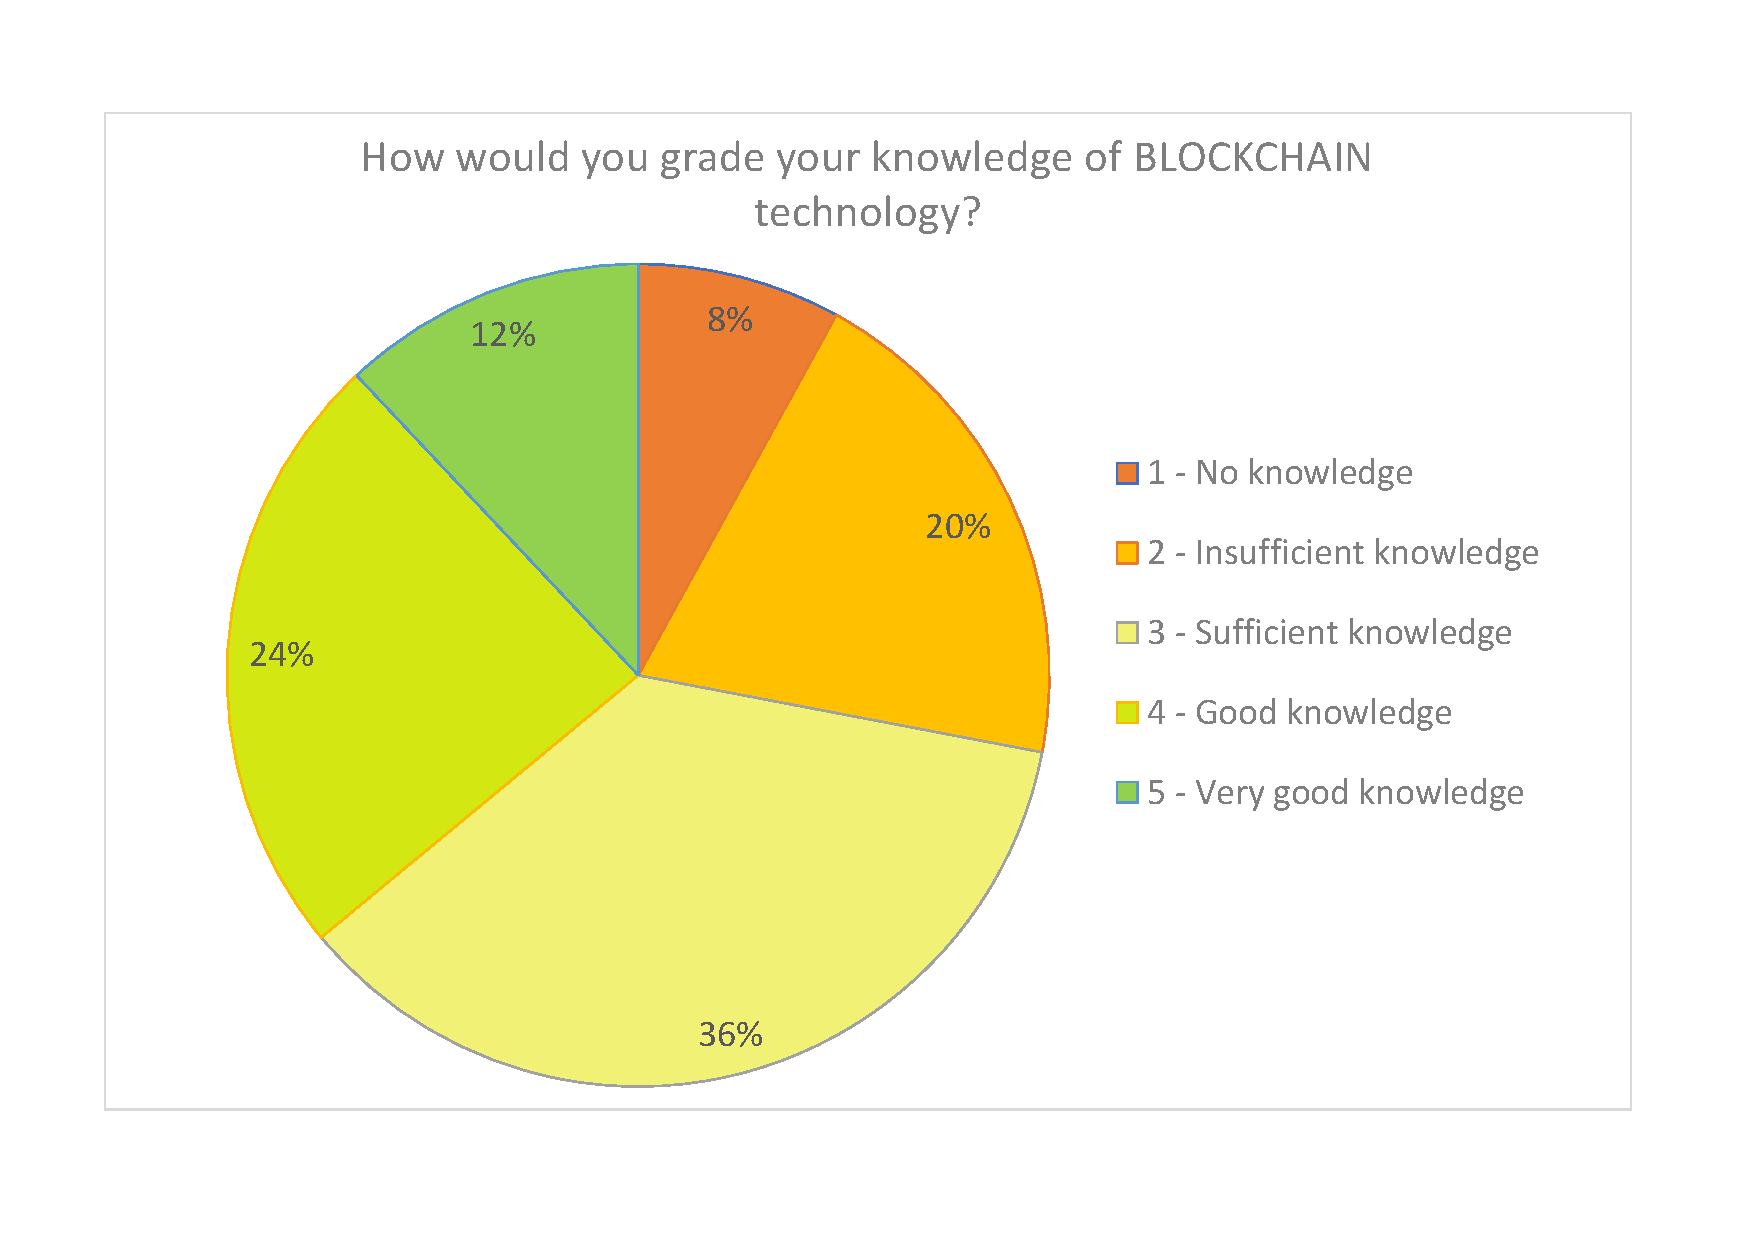
\includegraphics[scale=0.65]{media/survey_group2/blockchain_knowledge.pdf}
\caption{Question about Blockchain knowledge.}
\label{fig:blockchain_knowledge}
\end{figure}

In Figure~\ref{fig:blockchain_knowledge}, it can be seen that most answers are in the middle of the scale, while both the extremes have few answers, which closely resemble a gaussian or normal distribution. 

Indeed, when calculated, the skew of this data is about -0,065104294, which is a very low number (the standard error was about 0,46) and close to 0. A normal distribution has a skew of 0, so this can be said to be a good approximation. Additional, it can be said that there is not much of a bias towards accepting or denying blockchain when answering other questions, either from knowing too much or too little, since the knowledge curve seems to be normal.
 
\subsection*{2 - Rate the affirmations about the use of cryptocurrencies in the blockchain.}

After inquiring about the blockchain knowledge of the respondents, some affirmations were made about cryptocurrencies, which can be seen below. The question was optional, since respondents without sufficient knowledge of blockchain might face difficulties understanding the affirmations.


%GRAFICOS DE CADA 1 DAS 3 AFIRMAÇÕES DE CRYPTOCURRENCIES
\textbf{Affirmations: }
\begin{enumerate}
\item A blockchain always needs to have a cryptocurrency attached in order to work well.
\item Cryptocurrencies are useful in blockchains open to the public, in order to create incentives for good behavior, but not always necessary in private chains.
\item Blockchains can be useful in some uses cases, independently of whether they hold a cryptocurrency or not.
\end{enumerate}

Independently, these affirmations do not hold an absolute value that can help ascertain if there is a need for a cryptocurrency in the case of supply chain. But together, the three affirmations lead to a higher degree of certainty.

The first affirmation states that a blockchain, any at all, independently of the purpose or type, does indeed need a cryptocurrency. The second affirmation goes on a tangent from the first one, stating that maybe cryptocurrencies are only needed as an incentive, and otherwise could be not needed. The final affirmation is more generic in nature, and attempts to \textbf{completely separate the concept of blockchain and cryptocurrency}. The results for each affirmation can be found in Figure~\ref{fig:blockchain_crypto_opinions}. %and in Table~\ref{table:blockchain_crypto_opinions}.
\todo{pedro: where is the table???}
\begin{figure}[h]
\centering
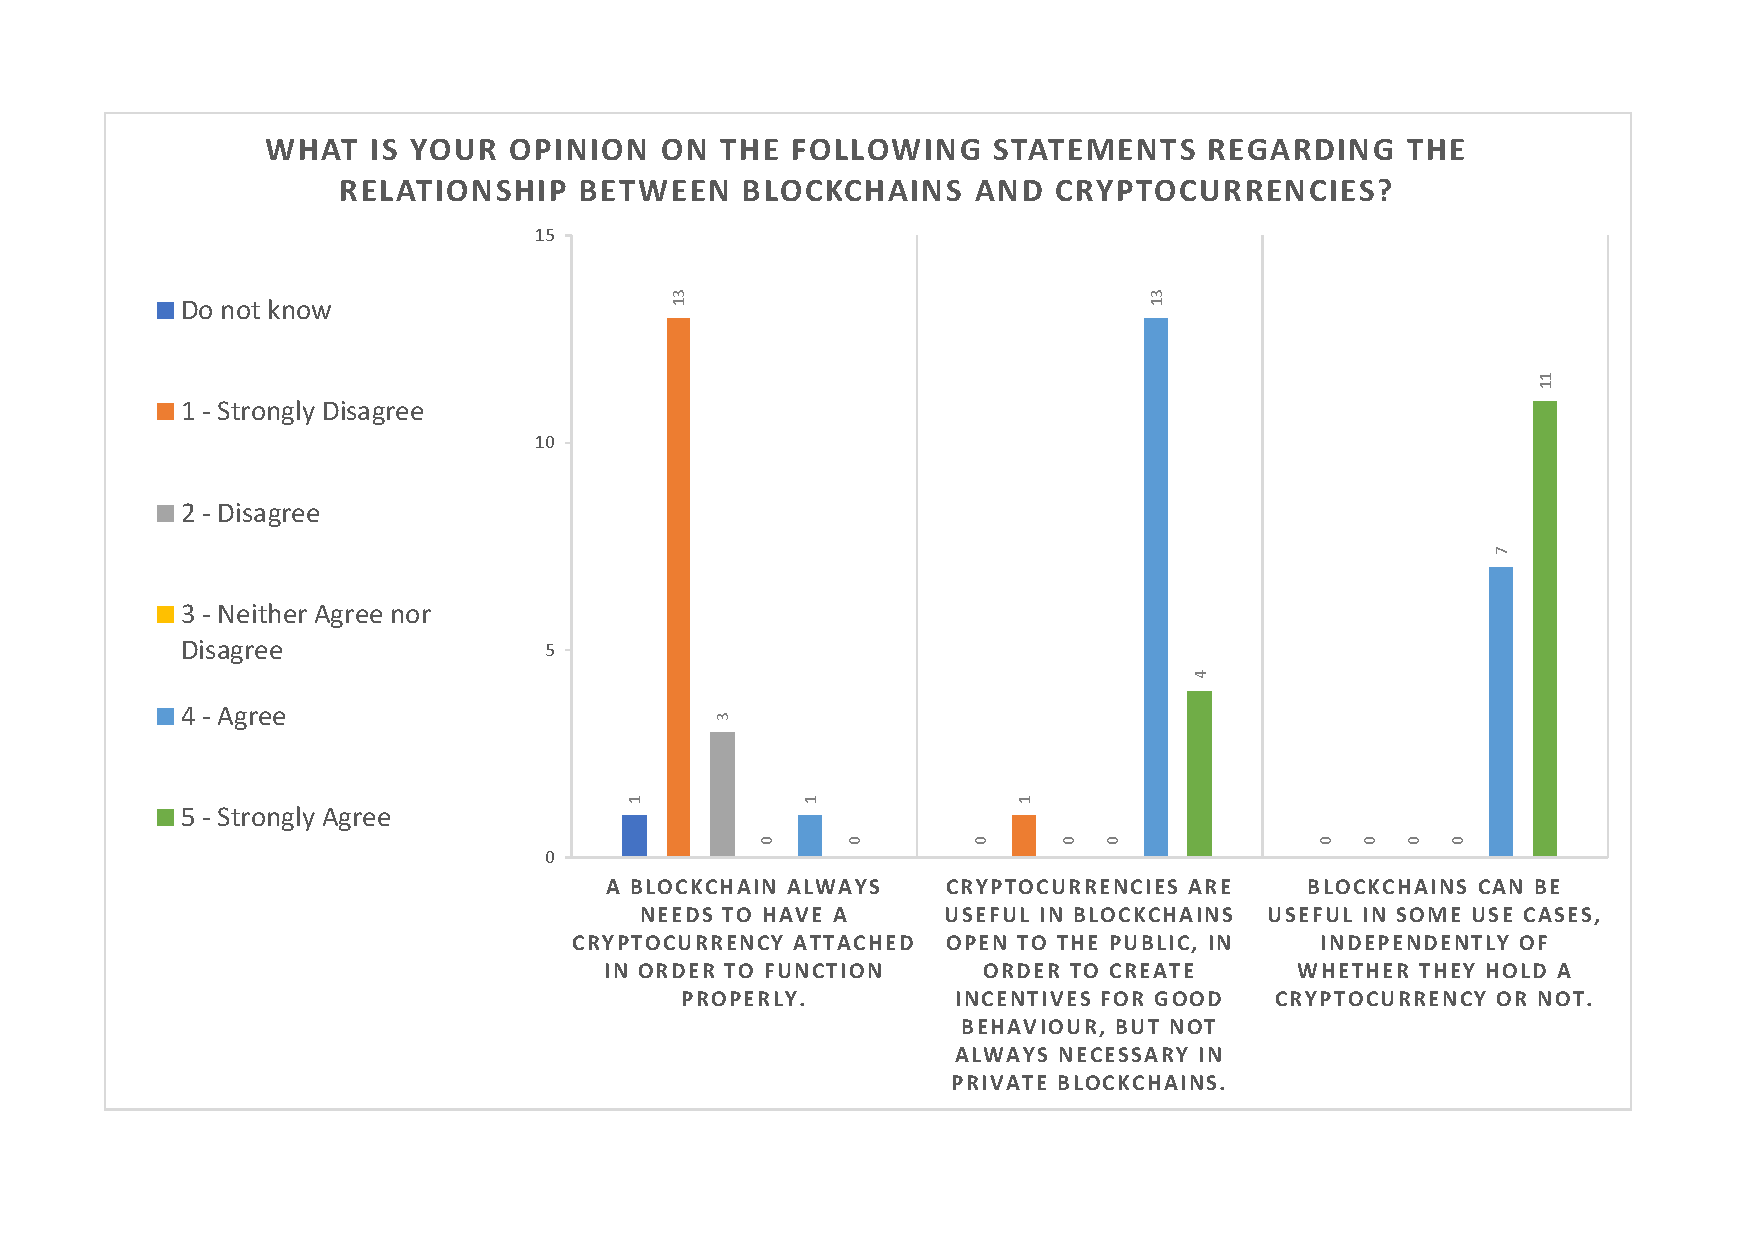
\includegraphics[scale=1]{media/survey_group2/blockchain_crypto_opinions.pdf}
\caption{Question to rate affirmations about the use of cryptocurrencies in the blockchain.}
\label{fig:blockchain_crypto_opinions}
\end{figure}



%%%%%% TABLE START %%%%%%%%%%%%%%
% Please add the following required packages to your document preamble:
% \usepackage[normalem]{ulem}
% \useunder{\uline}{\ul}{}
\begin{table}[ht]
    \centering
    \caption{My caption}
    \label{my-label}
    \begin{tabular}{l|c|c|c|c|c|c|}
    \cline{2-7}
                                                                                                                                                                & \multicolumn{1}{l|}{Mode} & \multicolumn{1}{l|}{Median} & \multicolumn{1}{l|}{Mean} & \multicolumn{1}{l|}{\begin{tabular}[c]{@{}l@{}}Standard\\  Deviation\end{tabular}} & \multicolumn{1}{l|}{Range} & \multicolumn{1}{l|}{Skewness} \\ \hline
    \multicolumn{1}{|l|}{\begin{tabular}[c]{@{}l@{}}1. Blockchain needs \\ cryptocurrencies to work well\end{tabular}}                                          & 1                         & 1                           & 1,36                      & 0,79                                                                               & 3                          & 2,74                          \\ \hline
    \multicolumn{1}{|l|}{\begin{tabular}[c]{@{}l@{}}2.  Cryptocurrencies are only \\ useful as incentives in public \\ blockchains\end{tabular}}                & 4                         & 4                           & 4,06                      & 0,87                                                                               & 4                          & -2,51                         \\ \hline
    \multicolumn{1}{|l|}{\begin{tabular}[c]{@{}l@{}}3. Blockchains can be useful in\\ some cases, regardless of having \\ or not cryptocurrencies\end{tabular}} & 5                         & 5                           & 4,61                      & 0,50                                                                               & 1                          & -0,50                         \\ \hline
    \end{tabular}
    \end{table}
%%%%%%%%%%% TABLE END %%%%%%%%%%%%%%%%%%%%%%%%%%%

\begin{itemize}
    \item The first affirmation has a very low agreement rate. Almost all of the respondents answered that they strongly disagreed with it, which can be seen in the table, as both the mode and median are 1, and the mean is also close to it. It can be concluded that, according to these opinions, \textbf{blockchain can sometimes not have a cryptocurrency and still perform well}.
    \item The second affirmation has a high agreement rate, with an average of 4.06. The mode and mean are also very close to the mean, and the standard deviation is lower than 1, which means that there is a consensus on the responses. Therefore, it can be concluded that, as per the opinions of the professionals, \textbf{a cryptocurrency is more useful in public blockchain contexts and applications, as an incentive, than in private blockchains, where these incentives are not needed.}
    \item The last affirmation has a very high agreement rate, the highest of them, with a mode and median of 5, and a mean of 4.61. There is a strong consensus, as all of the respondents answered with either 4 or 5 (Agree or Strongly Agree), leading to a low standard deviation and range. There is a slight skew, since the answers are distributed between these 2 items, with a bigger number of responses  on item 5. The conclusion for this affirmation is that \textbf{blockchains are useful, independently of holding a cryptocurrency or not}.
\end{itemize}


\subsection*{Conclusions from Question Group 2}

With these conclusions in mind, one final conclusion can be derived. If blockchains do not need cryptocurrencies to perform well (concluded from the non agreement with affirmation 1) and can generally still be useful without them (affirmation 3), then \textbf{cryptocurrencies should not be considered a necessity, but rather a design option, depending on the benefits} it can bring to a particular use case. Taking this conclusion into account, and also according to the agreement with affirmation 2, then: \textbf{if a blockchain design features a private blockchain, it does not necessarily need a cryptocurrency as a requirement, since incentives are not needede pointed out}. This is an especially interesting conclusion for the proof-of-concept.

%\subsection*{3 - Blockchain adoption challenges - maybe this one isnt that important to show}
% MAYBE TAKE THIS ONE OUT - NOT THAT IMPORTANT

\subsection{Question Group 3 - Supply Chain Points of Focus and Problems}
\label{sec-supplychainissues}
%GRAFICO Inventory management
This part of the survey focuses on finding out if the issues dug out on the background and pointed out in the Problem Statement chapter are really the ones that plague supply chain management. As such, a battery of questions including the various concerns mentioned was given to the respondents.

\subsection*{1 - Speed of Delivery, synchronization and traceability issues}

The respondents were asked the following 2 questions, as well as some affirmations to classify their agreement with.

\par\textbf{Questions:}
\begin{enumerate}
  \item In your experience, how frequently does the absence of crucial information cause delays in processes such as shipping, packaging, etc.?
  \item How important is Inventory Management for the efficiency of the supply chain?
\end{enumerate}

\par\textbf{Affirmations:}
\begin{enumerate}
%GRAFICO DAS 4 PRIMEIRAS RATE THE AFFIRMATION+FREQUENCY OF DELAYS (speed of delivery, synchronization,

\item In a supply chain, if the information gap between partners is shortened, a faster product cycle (or shorter lead time) can be attained.
\item Distribution, supply, demand and inventory planning all rely heavily on the information being both accurate and up to date

\item Supply Chain Management lacks a way to quickly and seamlessly share between companies all the information generated by the flow of assets in a Supply Chain.
\end{enumerate}

The data collected from these questions can be visualized in the graphs from Figure ~\ref{table:group3_graphics}. The data for the affirmations can be visualized in the graphs from Figure~\ref{fig:group3_graphics_2} and was summarized in Table~\ref{table:group3_graphics}.

\begin{figure}[h]
    %\makebox[2pt]{}
    \resfig{survey_group3/inventory_management_importance}{Inventory Management Importance}
    \resfig{survey_group3/absenceinfo_delays_affirmation}{Relation between the absence of information and delays}

      \caption{Questions to rank inventory management importance and relationship between absence of information and delays.}
    \label{fig:group3_graphics}
\end{figure}

\begin{figure}[h]
\resfig{survey_group3/information_gap_affirmation}{Relation between information gap and delays}
\resfig{survey_group3/planning_accuracy_affirmation}{Relation between management planning and information accuracy}
\resfig{survey_group3/quickinfo_sharing_affirmation}{Affirmation about the lack of a system with good integration of information}
\caption{Questions to rate affirmations about the effects of information gaps, the reliability of management planning and lack of a system with good integration.}
    \label{fig:group3_graphics_2}
\end{figure}

\begin{table}[h]
  \centering
  \caption{Question results metrics for the affirmations about the effects of information gaps, the reliability of management planning and lack of a system with good integration.}
  \label{table:group3_graphics}
  \resizebox{\textwidth}{!}{
  \begin{tabular}{l|c|c|c|c|c|c|}
  \cline{2-7}
                                                                                                                                                                                                                                                            & \multicolumn{1}{l|}{Mode} & \multicolumn{1}{l|}{Median} & \multicolumn{1}{l|}{Mean} & \multicolumn{1}{l|}{\begin{tabular}[c]{@{}l@{}}Standard\\  Deviation\end{tabular}} & \multicolumn{1}{l|}{Range} & \multicolumn{1}{l|}{Skewness} \\ \hline
  \multicolumn{1}{|l|}{\begin{tabular}[c]{@{}l@{}}Affirmation 1 - A reduction\\  of the information gap\\  between partners can lead \\ to a faster product cycle.\end{tabular}}                          & 5                         & 4                           & 3,92                      & 1,26                                                                               & 3                          & -1,21                         \\ \hline
  \multicolumn{1}{|l|}{\begin{tabular}[c]{@{}l@{}}Affirmation 2 - Distribution, \\ supply, demand and inventory \\ planning all rely heavily on \\ the information being both \\ accurate and up to date.\end{tabular}}                                       & 5                         & 5                           & 4,64                      & 0,49                                                                               & 1                          & -0,62                         \\ \hline
  \multicolumn{1}{|l|}{\begin{tabular}[c]{@{}l@{}}Affirmation 3 - Supply Chain \\ Management  lacks a way to \\ quickly share between\\  companies all the information \\ from the supply chain.
  \end{tabular}} & 4                         & 4                           & 3,79                      & 0,83                                                                               & 3                          & -0,56                         \\ \hline
  \end{tabular}
  }
  \end{table}

\pagebreak

Beginning with the analysis of the 2 questions:
\begin{itemize}
  \item The first question had the objective of finding out whether Inventory Management is an important discipline for the efficiency of the supply chain, which is an important aspect, if it is to be treated as point of possible improvement. The data was ranked from 1 to 5, with 1 being "Not at all important" and 5 being "Very Important". The question scored a mean of 4.48, with the mode and median both being 5, since most results sit on that score. There is little dispersion in the results, with most of the other answers scoring a 4 and only 1 answer scoring a 3. It can be concluded that \textbf{Inventory Management is an essential discipline for supply chain management, according to the professionals.}
  \item The second question tries to relate the absence of information with delays in the processes of sending products. The scale went from 0 to 10, which corresponded from the percentages 0 to 100\%. The final results ranged from 40\% to 90\%, with most of the answers sitting between 60\% and 80\%. The results were not very spread out, with a standard deviation of only 1.29, in the scale of 1 to 10. There were not also any significant outlier values, with the skew being classified as normal, with a value below the threshold of the standard error. \textbf{The average result for this opinion was 68\%, which is a reasonably high percentage that we can say there might really be correlation between these 2 aspects, especially given the consensus and non-existence of outlier values. However, this can never be said with total certainty, since these are only opinions and not factual data}. 
\end{itemize}
%We know that Inventory management relates to lots of practices, and these are important


A follow-up with the analysis of the opinions about the affirmations:
\begin{itemize}
  \item The first affirmation related a reduction in the information gap with a faster product cycle. In layman's terms, this can be thought of as "if there is more information available, the products will get made faster, shipped faster and received faster". Many respondents seemed to only cautiously agree with the affirmation, not committing to a strong answer. Even though the most popular answer was 5, the mean still was below the normal agreement level, at 3.92. There is some skew and spread, due to the lower results, but these still look like valid answers. Therefore, it can be informally generalized that \textbf{while it may be true indeed that having information available will generally help products finish their cycle faster, it might not always be the case, as there is not a strong consensus about this.}
  \item The second affirmation relates all the planning disciplines in SCM with the existence of up-to-date and accurate information. The respondents all answered with either 4 or 5, a very low spread of answers, with most of them strongly agreeing (agreement average of 4.64. It can then be concluded that having accurate and up-to-date information is essential for these planning management tasks, which, of course, affect inventory management, which we already concluded to also be essential. \textbf{It is, therefore, of the utmost importance for a supply chain to be provided timely with exact information}.
  \item The last affirmation states that supply chain management might lack a way to integrate the information provenient from the flow of assets between companies easily. However, out of the 3 affirmations, this is the one with the lowest agreement of them. While the average agreement, 3.79, is close to the one from the first affirmation, the most popular choice here was 4 (Agree), followed by 3 (Neutral). The skew is almost low enough that this would represent a normal distribution for the answer. \textbf{While it seems that not every professional agrees, and some think that there are already good ways to integrate information quickly and seamlessly, the majority still thinks that SCM is lacking on this aspect.}
\end{itemize}

\subsection*{2 - Quality assurance and traceability issues}

Finally, with the objective of ascertaining whether quality assurance is also an issue, the respondents were asked 2 questions, with the results being shown in Figure~\ref{fig:group3_quality}. The first, similarly to previously, was asking about the agreement with an affirmation, and the second was a question.  Both the affirmation and question are as follows:

\begin{enumerate}
  \item Non-compliance with certain standards is a big issue that affects the reputation of companies working with sensitive products.
  \item In your experience, do you think that compliance with quality standards would be easier to achieve if all the products were traced as well as the processes they go through?
\end{enumerate}

\begin{figure}[h]
  %\makebox[2pt]{}
  \resfig{survey_group3/noncompliance_reputation_affirmation}{Relation between standard non-compliance and company reputation}
  \resfig{survey_group3/quality_traced_affirmation}{Relation between process traceability and quality standards compliance}

    \caption{Questions about quality assurance issues.}
  \label{fig:group3_quality}
\end{figure}
%GRAFICOS DAS 2 PERGUNTAS DE QUALITY ASSURANCE (traceability)

Looking at the graphics, the second question has a slightly higher agreement rate than the first one. However, both questions have very high agreement results, with absolutely no disagreement answers and only 1 neutral answer on the second question. It can be concluded that \textbf{quality standards compliance might affect a company's reputation and is also somewhat dependent on the traceability of products and processes they go through}.


\subsection*{Conclusions from Question Group 3}

\begin{itemize}
  \item From the first set of questions, we summarily conclude that the accurate synchronization of data and the speed of delivery (metrics stated in the problem statement) are related and an improvement in the synchronization might positively affect the speed of delivery, as well as other important metrics of a product's cycle. Though there may be solutions for this, the professionals still that they might be lacking.

  \item From the second set of questions, the only conclusion was that companies have in their interest to follow the quality standards, and traceability plays a big role in this.
\end{itemize}

The questions from this group have successfully validated most, if not all, of the supply chain issues raised in the previous chapters. The remaining questions from the survey point towards points of improvement for these issues, as well as what possible features to implement in a system could help with these issues.

\subsection{Question Group 4 - Supply Chain Standalone Points of Improvement and Blockchain points of Applicability and Improvement for Supply Chain}
\label{sec-survey-improvement-functionalities}

The first goal for this part of the survey is to find out the points of improvement for supply chain. What is being questioned are not the issues of the supply chain themselves, which were already asked, but what parts of supply chain, even though they may already work well, could work even better.

The second goal is to find out more about the requirements that an information system must have to satisfy the needs of SCM. This includes ranking the functionalities of an information system for their importance. Many of these functionalities probably relate to the points of improvement found here, as well as to the supply chain issues described in Section~\ref{sec-supplychainissues}.

%Problema: há varios graficos para mostrar, mas alguns deles, como o da figura 6.1, têm varias (7 a 8) distribuições para mostrar, onde cada uma delas tem os seus valores das metricas.

%2 EM 1
%GRAFICOS DOS SUPPLY CHAIN IMPROVEMENT ASPECTS


For the sake of simplifying the ranking process for both the \textit{"points of improvement"} and \textit{"functionalities of an information system"}, a division into groups of importance shall be done according to the observed results. The importance scale went from 1 to 5, but most of the mean scores were between 3 and 4.5. 

Therefore, the following classification for the lists of results will be adopted: 

\begin{itemize}
    \item \textbf{Mean 	$\geq$ 4} - High priority or importance
    \item \textbf{3.5 $\leq$ Mean $<$ 4} - Medium importance 
    \item \textbf{Mean $<$ 3.5} - Low importance
\end{itemize}

\subsection*{1 - Rank the importance of some aspects which Supply Chains aim to improve.}
 
%Dividir em mais imagens?
%\todo{fcorreia: sim, está muito pequeno para se ler assim. talvez quatro ou cinco destes gráficos lado a lado fiquem ok...}

\begin{figure}[h]
\centering
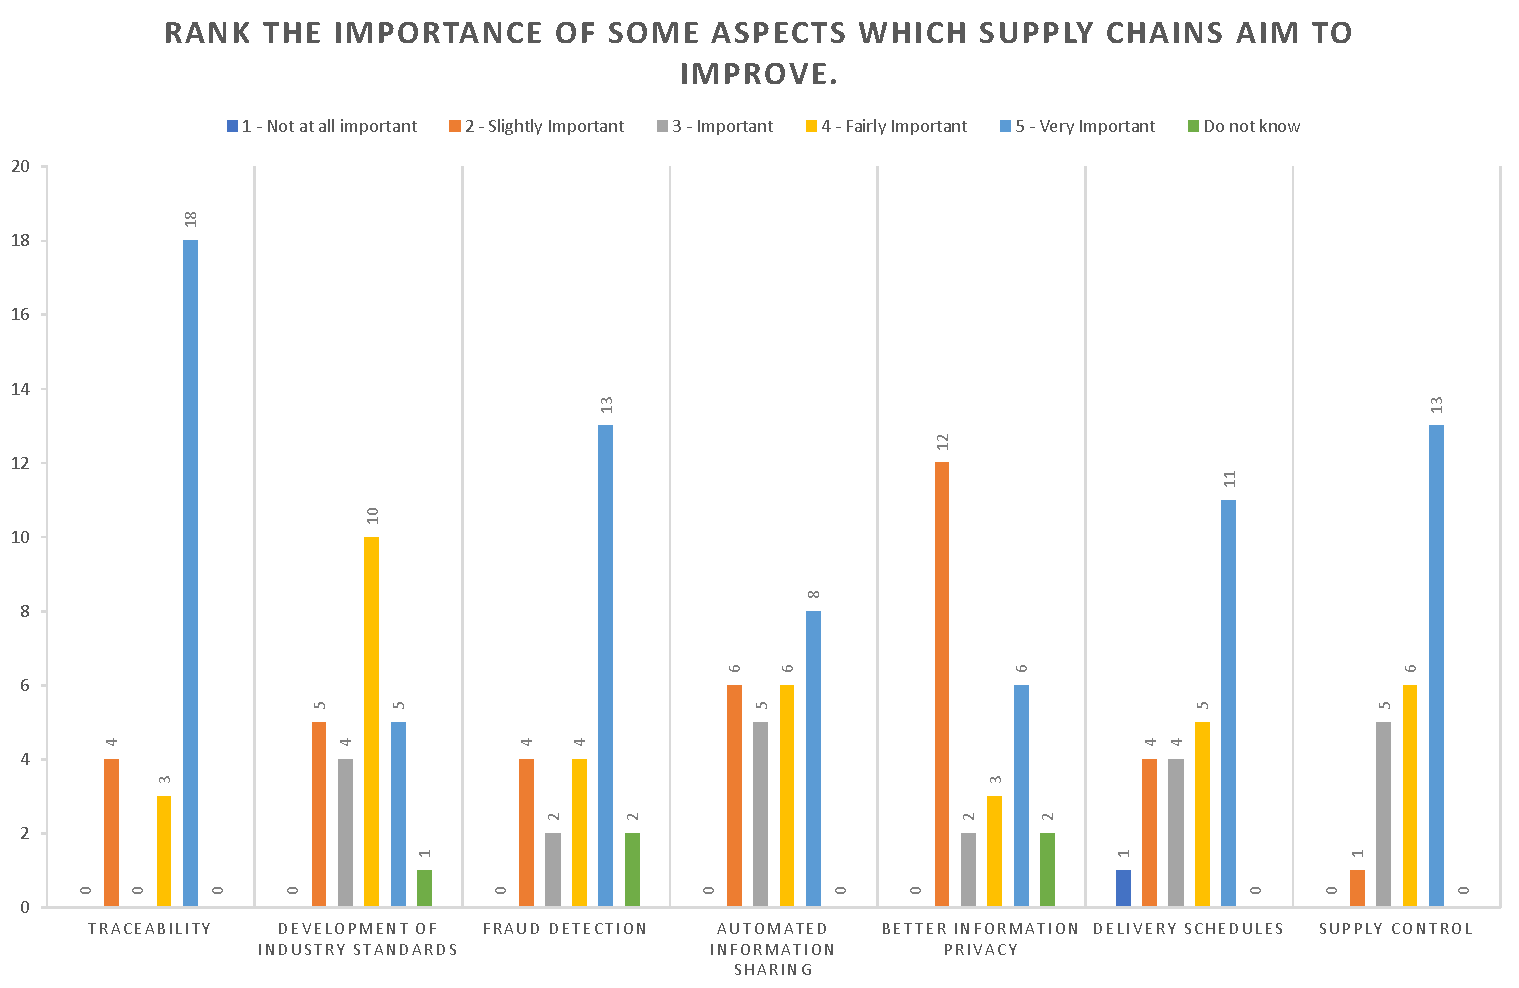
\includegraphics[scale=0.60]{media/survey_group4/importance_SC_improvement_points.pdf}
\caption{Question: "Rank the importance of some aspects which Supply Chains aim to improve."}
\label{fig:importance_SC_improvement_points}
\end{figure}

%%%%%%%% TABLE BEGIN %%%%%%%%%

\begin{table}[h]
\centering
\caption{Question results metrics for the question to rank the importance of improvement aspects of the supply chain.}
\label{table:metrics-importance-improvement-sc}
\resizebox{\textwidth}{!}{
\begin{tabular}{l|l|l|l|l|l|l|}
\cline{2-7}
                                                                                                    & Mode & Median & Mean   & \begin{tabular}[c]{@{}l@{}}Standard\\ Deviation\end{tabular} & Range & Skewness \\ \hline
\multicolumn{1}{|l|}{Traceability}                                                                  & 5    & 5      & 4,40  & 1,12                                                       & 3     & -1,67  \\ \hline
\multicolumn{1}{|l|}{\begin{tabular}[c]{@{}l@{}}Development\\ of Industry\\ Standards\end{tabular}} & 4    & 4      & 3,63 & 1,06                                                       & 3     & -0,36  \\ \hline
\multicolumn{1}{|l|}{\begin{tabular}[c]{@{}l@{}}Fraud\\ Detection\end{tabular}}                     & 5    & 5      & 4,13 & 1,18                                                       & 3     & -1,00  \\ \hline
\multicolumn{1}{|l|}{\begin{tabular}[c]{@{}l@{}}Automated\\ Information \\ Sharing\end{tabular}}    & 5    & 4      & 3,64 & 1,19                                                       & 3     & -0,200  \\ \hline
\multicolumn{1}{|l|}{\begin{tabular}[c]{@{}l@{}}Better\\ Information\\ privacy\end{tabular}}        & 2    & 2      & 3,13 & 1,32                                                       & 3     & 0,51   \\ \hline
\multicolumn{1}{|l|}{\begin{tabular}[c]{@{}l@{}}Delivery\\ Schedules\end{tabular}}                  & 5    & 4      & 3,84 & 1,28                                                       & 4     & -0,71  \\ \hline
\multicolumn{1}{|l|}{Supply Control}                                                                & 5    & 5      & 4,24 & 0,926                                                       & 3     & -0,87  \\ \hline
\end{tabular}
}
\end{table}

%%%%%%%% TABLE END %%%%%%%%%%%%%%%%

In this category, we can see the results on Table~\ref{table:metrics-importance-improvement-sc}. Pretty much all the options had a range of 3 and deviations close to 1, which is to be expected. Traceability had the highest skew value, as there seemed to be some dissent, as a few outlier values pushed the mean to be lower than the median. However, it still rated the highest, by importance. 

The importance ranking described as before follows below:

\begin{enumerate}
    \item \textbf{High importance} - "Traceability", "Supply Control", "Fraud Detection";
    \item \textbf{Medium importance} - "Delivery Schedules", "Automated Information Sharing", "Development of Industry Standards"
    \item \textbf{Low importance} - "Better Information Privacy"
\end{enumerate}

\par \textbf{Conclusions: }
%Points of failure from before: traceability, inventory management is ESSENTIAL
\begin{itemize}

\item High Importance - It had already been concluded from the previous set of questions in~\ref{sec-supplychainissues} that inventory management was an essential discipline to SCM, so it was expected that \textit{Supply Control} would be rated highly as a point of improvement, which it did. The same can be said about \textit{Traceability}: it was expected to rank highly, since it is related to both quality assurance and availability of information, two other issues that were validated in the previous set of questions. At the same time, \textit{Fraud Detection} was also highly ranked, which can be explained by its relation to traceability and quality compliance and control. \textbf{Traceability helps to avoid fraud and, at the same time, fraud detection also relates to quality control and compliance, since avoiding fraud is all about making sure that the products circulating the supply chain are authentic and have good quality.} With this in mind, it is only natural that Fraud Detection is considered important, together with traceability.

\textbf{In conclusion, the 3 most important items are traceability, supply control and fraud detection, with supply control and fraud detection directly depending on the traceability, which makes traceability probably the most important point of improvement in the supply chain.}

\item Medium Importance - From the items that got rated as medium importance, 2 of them relate to synchronization improvement: \textit{Automated Information Sharing} and \textit{Development of Industry Standard}. The last point, \textit{Delivery Schedules} also relates to Supply Control, though it is less generic.

\textbf{In conclusion, though system synchronization is not as important as traceability or some of the other items that depend on traceability, it is still a welcome improvement which comes in second place to the others.}


\item Low Importance - Finally, the lowest ranking item was \textit{Better Information Privacy}. This comes as a surprise, since security was a big focus on the background research for supply chain management. 

\textbf{The conclusion we can take from this item being rated the lowest, is that it might be a concern that the current systems already take care of, therefore it does not have much space for improvement.}
\end{itemize}


%2 EM 1https://www.overleaf.com/13104200fnmytzmhwtck#
%GRAFICOS DOS BLOCKCHAIN POINTS OF APPLICABILITY
\subsection*{2 - Rank the importance of the following functionalities for an information system that stores or processes data pertaining to a Supply Chain}

\begin{figure}[h]
\centering
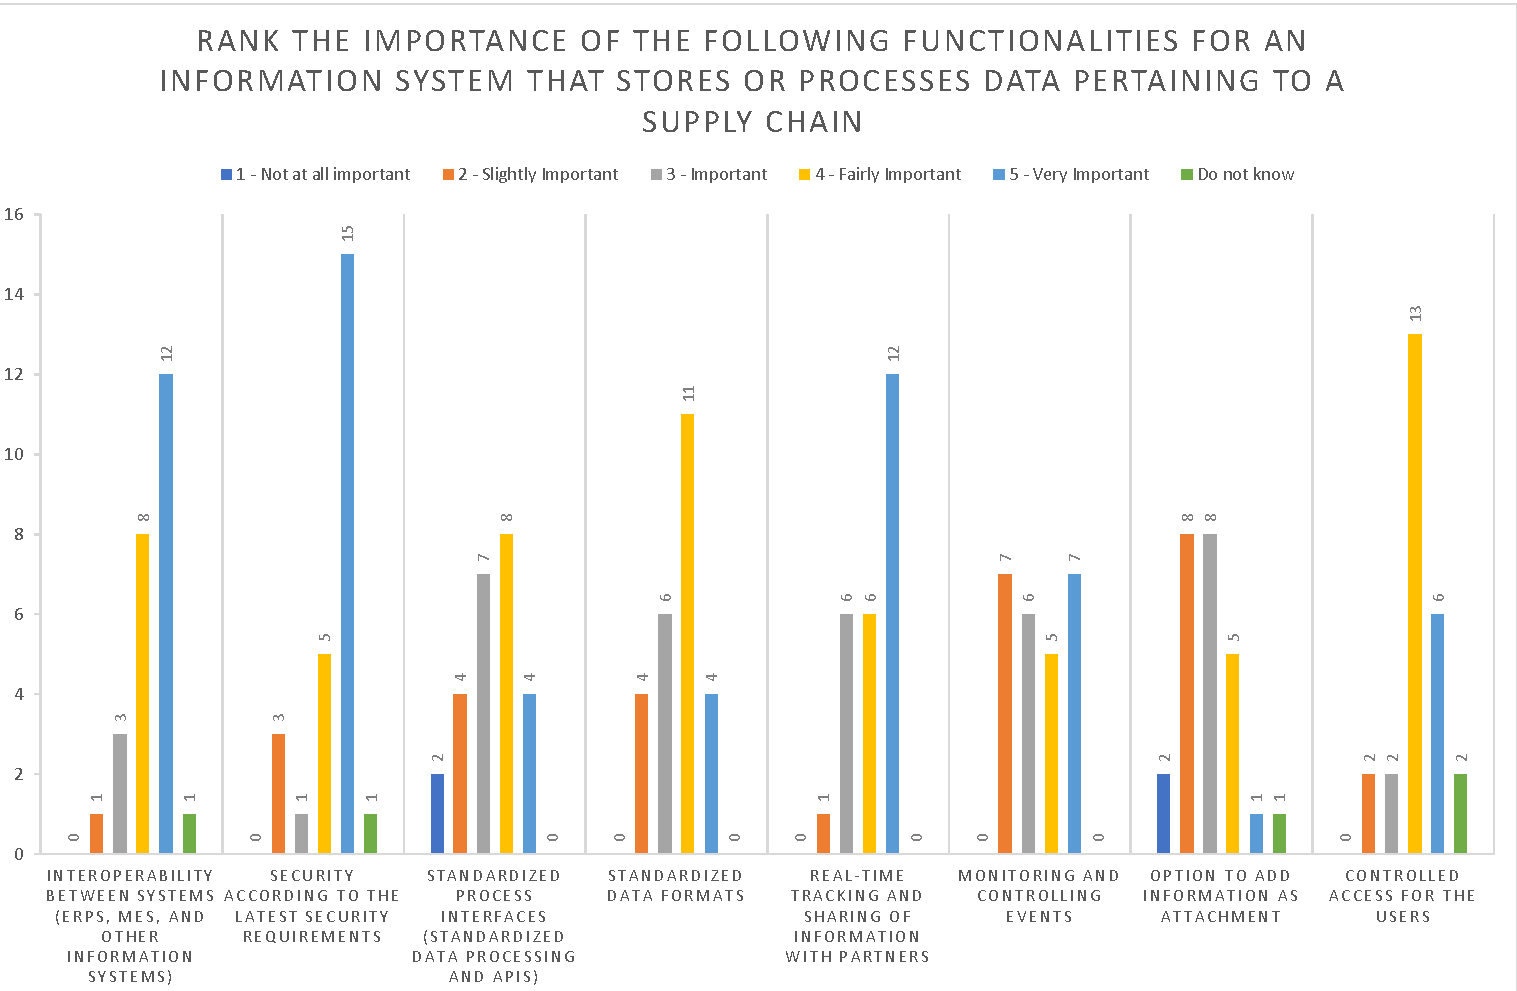
\includegraphics[scale=0.60]{media/survey_group4/importance_SC_info_systems.pdf}
\caption{Question: "Rank the importance of some functionalities in a supply chain based information system."}
\label{fig:importance_SC_info_systems}
\end{figure}

%%%% TABLE START %%%%%%%%%%

\begin{table}[h]
\centering
\caption{Question results metrics for the question to rank the importance of functionalities in an information system for supply chain.}
\label{table:metrics-importance-info-systems}
\resizebox{\textwidth}{!}{
\begin{tabular}{l|c|c|c|c|c|c|}
\cline{2-7}
                                                                                                                                                & \multicolumn{1}{l|}{Mode} & \multicolumn{1}{l|}{Median} & \multicolumn{1}{l|}{Mean} & \multicolumn{1}{l|}{\begin{tabular}[c]{@{}l@{}}Standard\\  Deviation\end{tabular}} & \multicolumn{1}{l|}{Range} & \multicolumn{1}{l|}{Skewness} \\ \hline
\multicolumn{1}{|l|}{\begin{tabular}[c]{@{}l@{}}Interoperability Between \\ Systems (ERPs, MES, \\ and other information systems)\end{tabular}} & 5                         & 4,5                         & 4,29                    & 0,86                                                                             & 3                          & -1,08                       \\ \hline
\multicolumn{1}{|l|}{\begin{tabular}[c]{@{}l@{}}Security according to the\\  latest security requirements \end{tabular}}                                               & 5                         & 5                           & 4,33                    & 1,05                                                                             & 3                          & -1,49                       \\ \hline
\multicolumn{1}{|l|}{\begin{tabular}[c]{@{}l@{}}Standardized Process Interfaces \\ (Data Processing and APIs)\end{tabular}}                     & 4                         & 3                           & 3,32                    & 1,18                                                                            & 4                          & -0,36                       \\ \hline
\multicolumn{1}{|l|}{Standardized Data Formats}                                                                                                 & 4                         & 4                           & 3,60                    & 0,96                                                                             & 3                          & -0,31                       \\ \hline
\multicolumn{1}{|l|}{\begin{tabular}[c]{@{}l@{}}Real-time tracking and sharing \\ of information with partners\end{tabular}}                    & 5                         & 4                           & 4,16                    & 0,94                                                                             & 3                          & -0,67                       \\ \hline
\multicolumn{1}{|l|}{Monitoring and controlling events}                                                                                         & 5                         & 3                           & 3,48                    & 1,19                                                                             & 3                          & 0,05                       \\ \hline
\multicolumn{1}{|l|}{\begin{tabular}[c]{@{}l@{}}Option to add information \\ as attachment\end{tabular}}                                        & 2                         & 3                           & 2,79                    & 1,02                                                                             & 4                          & 0,19                        \\ \hline
\multicolumn{1}{|l|}{Controlled access for the users}                                                                                           & 4                         & 4                           & 4                         & 0,85                                                                             & 3                          & -0,96                       \\ \hline
\end{tabular}
}
\end{table}


Results for this question are found in Figure~\ref{fig:importance_SC_info_systems}, and the analysis metrics are in Table~\ref{table:metrics-importance-info-systems} the range of answers is pretty much 3 for all options but 2 of them. The mean and median of the items are also a close approximation of each other, which happens because the skew in most cases is  not very high (only for the Interoperability and Security items was it higher than 1). The skew is highest on the items that also had the highest mean. This happens because, even though these items are the most popular, there are always a few answers from people who disagree. However, this is to be ignored, given the low deviation and given that the median and mean are very close to each other in every case. Therefore, the mean can still be used here to classify the importance.

The importance ranking described as before follows below:

\begin{enumerate}
    \item \textbf{High importance} - "Security according to the latest requirements", "Interoperability Between Systems", "Real-time tracking and sharing of information", "Controlled access for the users";
    \item \textbf{Medium importance} - "Standardized Data Formats"
    \item \textbf{Low importance} - "Monitoring and controlling events", "Standardized Process Interfaces", "Option to add information as attachment"
\end{enumerate}

\par \textbf{Conclusions: }
\begin{itemize}

    \item 2 of the high importance items actually relate to security, namely access control and following security requirements. This contrasts with the point of improvement from the previous set of questions \textit{"Better information privacy"}, which was rated the lowest in relative importance. There seems to be a disparity between the importance of the functionality and the importance of the improvement, which might mean that the functionality is important but already good enough as it is.
    
    \textbf{The conclusion we can take is that keeping security up to date still seems to be considered important, but on aspects other than privacy (which is already fulfilled) such as access control, which relates to authorization and authentication.}

    \item The other 2 high importance functionalities were about interoperability between systems, and tracking and sharing information. Tracking and sharing information relates to traceability and information synchronization, while interoperability relates only to synchronization.

    \textbf{Though these points, which relate to synchronization scored high as a functionality, the points of improvement they relate to only scored as medium in the previous sections, namely \textit{"Automated Information Sharing"} and \textit{"Development of Industry Standards"}. Thus, integrating the information is seen as an important aspect to have,but not one that needs improvement over the current status.}

\item Most of the items rated as having medium or low importance do not necessarily stand out nor do they have important conclusions to be taken. The one thing that stands out is that \textit{"Monitoring and controlling events"} rated as a low importance functionality, even though traceability rated high as a point of improvement, which does not make a lot of sense, since traceability also means having the means to monitor what is happening.


\end{itemize}

%%%% TABLE END %%%%%%%%%%

\subsection*{3 - Blockchain applicability to the supply chain}
 
%CHANGE IMAGES TO THE 2 GRAPHICS ABOUT USE CASES OF BC+SC AND BENEFITS OF BC+SC

The final important group of questions featured 2 questions about the viability of applying blockchain to the supply chain. The first question asked people which use cases they thought were the best for applying blockchain to the supply chain and respondents could select a maximum of 3 options (including "None" or "Do not know").

\begin{figure}[h]
    %\makebox[2pt]{}

	\resfig{survey_group4/blockchain_usecases_sc}{Blockchain use cases for the supply chain}
    \resfig{survey_group4/blockchain_application_benefits}{Blockchain benefits for the supply chain}
    
      \caption{Question: Blockchain use cases and benefits for the supply chain.}
    \label{fig:group4_graphics}
\end{figure}

\textbf{Starting with the analysis of the first question}:
\begin{itemize}
    \item \textbf{Financial transactions was, by far, the most popular choice.} The respondents look at blockchain as a way to move money as an asset, more than a tool to manage the goods themselves, since traditional systems only deal with data and the money is dealt with by third parties (banks). It makes sense that \textbf{the second most voted choice is Contract Enforcement.} As per the background research and state of the art, it was pointed out that some of the applications already enforce payments through contracts, when the goods are delivered,for instance, without the need of a third party (thus reducing fees). Financial transactions and contract management go hand in hand. 
     
    \item With the same number of votes, \textbf{also in second place, is "regulatory compliance and auditing"}. Regulatory compliance is a term also related to contracts enforcement. Contracts are used to establish mandatory rules which are automatically enforced according to the conditions of the system (for instance, enforce that the food transported in a truck never goes over a certain temperature value). \textbf{However, an important point to note is that regulatory compliance and auditing are made possible through the traceability characteristic of blockchain, which allows for products and processes to be thoroughly verified. This means that traceability is a highly sought after application of blockchain.}
    \item "Secure data storage" was also a highly voted option. Security is an important focus in information systems, so this should be taken into account when building the proof-of-concept. In the previous set of questions, "access control" and "security according to the latest requirements" were also features that stood out, so \textbf{it is not a surprise that secure data storage is seen as one of the main advantages of blockchain, since it boasts of being cryptographically secure, having immutability by design and an easy to implement access control.}. 

\end{itemize}

The proof-of-concept has to not only take these use cases into account as the main applications, but also implement (or make possible the implementation of) the most important features of information systems previously analyzed, which makes the second question complementary of the first one.

\textbf{For the second question, there is an analysis of the benefits that blockchain can bring to the supply chain, according to the respondents}:

\begin{itemize}
    \item The three most voted items were: \textit{"Better transaction integrity and visibility"}, \textit{"Reduction of risks (fraud/tampering/information leaks)"} and \textit{"Stronger working relationships with partners"}.

    The first two items were expected to rank high. They directly relate to the security and traceability, points of improvement already discussed - traceability makes it possible to view the records to make sure nothing suspicious is going on, and the security and immutability of the information makes it impossible to tamper with the data.
    
    The third point, "Stronger working relationships with partners", however, is interesting to see being chosen a high ranked benefit. The concept of strong relationships with partners is linked to  the concept of \textbf{internal supply chain trust}, which was already introduced in~\ref{sec:advantes-blockchain}. The ability for partners to trust each other is what makes the supply chain possible and efficient to the standards of today. It seems that the professionals really do think of blockchain as a tool to improve this internal trust.
    
    The selection of these 3 items as the most voted does not seem to be a coincidence. \textbf{Blockchain can be used as a source of truth for the supply chain and this leads to the side benefits of internal trust, better relationships with the partners, less fraud, less tampering, less leaks, among other benefits, all made possible because of the main characteristics: security and traceability.}
\end{itemize}

\subsection*{Conclusions from Question Group 4}

This was the most important group of questions in that it provides direct information as to which functionalities the proposed system design should possess and implement. At the same time, these functionalities can be related to the points of improvement found, as well as to the issues validated in the previous groups of questions.

\begin{itemize}
    \item From question group 3, some issues in the supply chain were validated: \textbf{inventory management}, \textbf{quality assurance} and \textbf{getting accurate and timely data}. On this group, the main points of improvement were found to focus on: \textbf{traceability}, \textbf{supply control}, \textbf{fraud detection} and \textbf{synchronization}. In a generalized way, the common links to both issues and points of improvement seem to be: \textbf{security}, \textbf{traceability} and \textbf{synchronization}, effectively validating the initial concerns from the problem statement.
    \item Another important conclusion to take from this set of questions are the features to include in the design for the blockchain system. These include the \textit{\textbf{"Blockchain only features"}}, functionalities implemented in an unique to the blockchain, as well as the standard \textit{\textbf{"Information system features"}}, which are the features that were found to be the most important to information systems in a supply chain.
    \item By order of importance, the blockchain features are:
    \begin{itemize}
        \item Financial transactions.
        \item Some form of regulatory auditing.
        \item Enforceable contracts (smart contract functionality).
        \item Secure data storage.
        \item Asset management.
    \end{itemize}
    \item By order of importance, the most important information system requirements are:
    \begin{itemize}
        \item Security according to the latest requirements.
        \item Interoperability between systems.
        \item Real-time tracking and sharing of information with partners.
        \item Controlled access for the users.
    \end{itemize}
\end{itemize}













\section{Conclusions}

\subsection{Survey Conclusions}
%Conclude that the prototype must focus on: security and traceability, as these are the items that the respondent's focused the most on; though these 2 are the focus, features such as X, Y, Z must not be forgotten, since they ranked high on both information system features and blockchain applicability to the SC; A good blockchain design for the SC should not only feature NEW use cases that the blockchain brings to SC, like financial transactions, but also feature improved features from the already existing systems.

Having analyzed all the groups of questions from the survey, it should now be possible to have an answer for the first question of the thesis sub-statements, presented in the problem statement: \textit{"What supply chain issues, improvements and requirements do the experts really find the most important?"}.

Most of the conclusions for the survey were summarized in the analysis of question group 4. These conclusions included the most important issues of the supply chain, points of improvement, blockchain features and information system functionalities important to the design.


\par \textbf{Issues} - These include \textbf{inventory management}, \textbf{quality assurance}, \textbf{} and \textbf{lack of accurate and timely data}. This last item was confirmed by the respondents to have a correlation to the lack of good integration and synchronization tools and to be one of the possible causes for the difficulties in planning management and product cycle delays.

\par \textbf{Point of improvement} - These include \textbf{traceability}, \textbf{supply control}, \textbf{fraud detection} and \textbf{synchronization}. These items reflect themselves on the feature requirements that were elicited. The results can therefore be crossed with the points of improvement to make more refined logical groups of requirements:

%%% TABLE START %%%%%%%%%%%
% Please add the following required packages to your document preamble:
% \usepackage{multirow}
\begin{table}[]
    \centering
    \begin{tabular}{|l|l|}
    \hline
    \textbf{Area}                                                                                              & \textbf{Requirements}                                                                                                              \\ \hline
    \multirow{3}{*}{Security}                                                                                  & Security according to the latest requirements                                                                                      \\ \cline{2-2} 
                                                                                                               & Controlled access for the users                                                                                                    \\ \cline{2-2} 
                                                                                                               & Secure data storage                                                                                                                \\ \hline
    \multirow{4}{*}{Traceability}                                                                              & Regulatory auditing                                                                                                                \\ \cline{2-2} 
                                                                                                               & Fraud detection                                                                                                                    \\ \cline{2-2} 
                                                                                                               & Asset management                                                                                                                   \\ \cline{2-2} 
                                                                                                               & Real-time tracking information                                                                                                     \\ \hline
    \multirow{3}{*}{Synchronization}                                                                           & Interoperability between systems                                                                                                   \\ \cline{2-2} 
                                                                                                               & Development of industry standards                                                                                                  \\ \cline{2-2} 
                                                                                                               & \begin{tabular}[c]{@{}l@{}}Real-time sharing of information with partners, leading to \\ better working relationships\end{tabular} \\ \hline
    \multirow{2}{*}{\begin{tabular}[c]{@{}l@{}}Transaction \\ Enforcement and\\ Financial domain\end{tabular}} & Financial transactions                                                                                                             \\ \cline{2-2} 
                                                                                                               & Enforceable contracts (smart contract functionality)                                                                               \\ \hline
    \end{tabular}
    \caption{Elicited requirements grouped by improvement area of focus.}
    \label{table:elicited-requirements-survey}
    \end{table}
%%% TABLE END %%%%%%%%%%%%%%%

These are important contributions from the experts of the area, though with a bigger sample, the answers would have been more representative. The next chapter will focus on these requirements as the major points of focus for the design.
%TODO: bigger conclusion




%subsection: relate to what the already existing projects do
\subsection{Comparison to the state-of-the-art projects}
Most of the projects analyzed in the state-of-the-art, thought they use a multitude of different frameworks and custom networks, also do not focus on satisfying all of the requirements, but mostly a subset of them. Most of the projects specialize only in 1 problem area, like traceability, instead of going for an all-rounded concept.

\par \textbf{CargoX} This project focuses somewhat on Secure Data Storage, Enforceable Contracts and Security, even though in a limited way, since the data stored is not for any asset or document, but specifically for bill of lading documents. Additionally, it lacks a lot in the traceability items.

\par \textbf{Eximchain} It attempts to tackle all of the areas: Traceability, Security, Synchronization, Contracts and Finance. Though it promises a lot in its presentations, the actual whitepaper and technical documents focus mostly on the financial and contractual aspects and do not explain how the other aspects will be achieved in detail. The product looks promising for this area, by focusing all the requirements in a way that is claimed to be efficient, with custom networks and consensus algorithms and protocols. However, and very importantly, Eximchain's product has not yet been proven to work. The project has 3 proof-of-concepts planned in their roadmap, each focusing on separate areas, but none has been presented yet.

\par \textbf{OriginTrail} This project boasts of its strong traceability capabilities, mainly for asset management, auditing and fraud detection. It is a specific project, but it does not fit all of the requirements above,  as it misses the financial transactions and some security aspects, such as access control. Again, as is the case with Eximchain, the project seems promising, but is yet to prove most of its functionalities, having released proof-of-concepts mostly for the traceability requirements. This seems to be a common element to most of these projects, in that they look promising but take a long time to prove that they can deliver their promises.

\par \textbf{Ambrosus} Focuses a lot on auditing, fraud detection, quality control and traceability in general, so it fills all the traceability requirements. Even though these features are a must, and seemingly the most important, most of the other requirements are not met, especially the financial transactions, asset management and part of the security requirements.

In summary, the existing projects are either very specialized and do not meet all the requirements, or they are very broad in the requirements, but in early stages of development, without proving that they can do what they promise.

	\chapter{Research Validation - Design and Implementation of a Prototype}
\label{chap:prototype}
\minitoc \mtcskip \noindent 



Following the conclusions and requirements elicited from the previous chapter, it is now time to answer the remaining two questions. The first question, \textbf{"What is the Blockchain tool or framework most adequate to the development of an architecture that can support these requirements?"} requires an analysis of the frameworks. The second question, \textbf{"Is it possible to build a feasible architectural design, by using such a tool, to implement all these requirements?"} requires that the elicited requirements be formed into a list and that an architectural design be built and implemented using the chosen framework. Only at the end of these tasks can the results be validated. 

This chapter deals with explaining these tasks sequentially. The first section analyzes which frameworks best satisfy the requirements and a choice is made. The second through fourth sections resemble a software engineering approach: starting in the requirements specification, following it up with the design, implementation using the framework and finally, the validation of the requirements.

However, due to time constraints, and also because the results from the survey took some time to collect, the requirements were written during the collection of these results and refined until after the results were finished being gathered and analyzed. At the same time, the implementation for these requirements was also being done, as it was more practical and efficient than to leave it for the end. Because of this, some requirements ended up being more emphasized in the design and implementation than some others that thee survey results would indicate to be more important.
\section{Framework Comparison and Choice}

Following the conclusions and requirements elicited in the previous chapter, it is now time to answer the second question from the problem statement: \textbf{What is the Blockchain tool or framework most adequate to the development of an architecture that can support these requirements?}

In order to make a good choice for the framework, there is a need to make a mixed analysis that focuses on the most important functionalities that an information system should feature as well as what use cases are most viable for applying blockchain to the supply chain.

In addition to the requirements from the previous chapter, the performance analysis from Chapter~\ref{sec-performance-comparison} should also be taken into account.

\subsection{Framework Requirements Elicited from the Survey}

The requirements for the choice of a framework can be partially derived from the most important functionalities pointed out on the results of the survey, in Table~\ref{table:elicited-requirements-survey}. These functionalities are directly based on some points of focus from this thesis: \textbf{synchronization, security and tracking or traceability}, so it is based on these attributes that the framework should also be selected.   

\par \textbf{Security}: From Section~\ref{sec-survey-improvement-functionalities}, it was ascerted that the improvement of information privacy in supply chains was not very important in itself. Maybe it is something that the current systems already do well, but as we can see, \textbf{there are still some outstanding concerns which deal with other security aspects that still need to be taken care of}: access control and fraud detection seem to rank high on the requirements for such a system. \textbf{Thus, the selected framework should support a highly controlled environment, where the actions each user takes should be properly authorized and there are good authentication mechanisms. Some fraud verification checks should be supported}.

\par \textbf{Traceability}: For the traceability requirements, the proposed system should be able to track all information, including changes in the system, registries of assets, transactions, network participants and organizations. It should also be open to outside regulatory entities, so that they can look into the system for auditing. Additionaly, sanity checks and other fraud-detection operations should be possible, possibly through smart-contract functionality. \textbf{Thus, the selected framework must support the management of data in the form of assets, entities and organizations, which should be accessible only to specific entities, including auditors}.

\par \textbf{Synchronization}: As the source of truth, the blockchain should be easily accessible to any external system that needs to query or insert data. The elicited requirements for synchronization include the development of standards and system interoperability for real-time sharing of the information. \textbf{Thus, the selected framework should easily expose the blockchain information to outside systems (for instance, through REST APIs) using predefined data formats}.

\par \textbf{Transaction Enforcement and Financial domain}: There is interest in financial applications, and cryptocurrencies are a part of this. However, for financial applications to be possible in the supply chain using blockchain, a native blockchain cryptocurrency is not necessarily needed, as cryptocurrencies can be simulated using balances, depending on the design of the blockchain network. For this, and other functionalities to work, smart contract functionality should exist, though. \textbf{Thus, the selected framework should either have a native cryptocurrency, or allow for the design of some kind of digital balance or token. Additionaly, it should support smart contracts}.


This information is summarized in Table~\ref{table-framework-requirements}.
%% Please add the following required packages to your document preamble:
% \usepackage{multirow}
\begin{table}[]
	\centering
	\begin{tabular}{|l|l|}
	\hline
	\textbf{Area}                                                                                              & \textbf{Framework Requirements}                                                                                    \\ \hline
	\multirow{3}{*}{Security}                                                                                  & Highly controlled environment                                                                                      \\ \cline{2-2} 
																											   & Authentication and authorization mechanisms                                                                        \\ \cline{2-2} 
																											   & Fraud verifications (by smart contracts)                                                                           \\ \hline
	\multirow{2}{*}{Traceability}                                                                              & Management of data: assets, entities, organizations                                                                \\ \cline{2-2} 
																											   & Data access controlled, but accessible to auditors                                                                 \\ \hline
	\multirow{2}{*}{Synchronization}                                                                           & Expose data to the outside systems through APIs                                                                    \\ \cline{2-2} 
																											   & Allow the use of predefine data formats                                                                            \\ \hline
	\multirow{2}{*}{\begin{tabular}[c]{@{}l@{}}Transaction \\ Enforcement and\\ Financial domain\end{tabular}} & Smart Contracts                                                                                                    \\ \cline{2-2} 
																											   & \begin{tabular}[c]{@{}l@{}}Native cryptocurrency or a way to simulate currencies or\\ account balance\end{tabular} \\ \hline
	\end{tabular}
	\caption{Summary of the framework requirements for each improvement area.}
	\label{table-framework-requirements}
	\end{table}
	
	%%%%%%%%%% TABLE END %%%%%%%%%%%%%%%%

\subsection{Framework Choice}

So, what conclusions can be taken from these framework requirements? Firstly, \textbf{a private blockchain framework seems more adequate}, because of all the security control mechanisms that are needed. Secondly, \textbf{the framework should allow for highly customizable networks, including not only asset management, but also identity management}, where the participants of the blockchain can be given specific permissions. Lastly, the framework needs to \textbf{allow the use of APIs}.

Crossing these requirements with the capabilities of the frameworks presented in the background chapters, we can do an analysis of the applicability of each one:
\begin{itemize}
	\item Ethereum - It is a public framework that features a native cryptocurrency and has strong financial capabilities. However, it costs money to run code on. Having a lot of the required functionalities on Ethereum would be a lot more expensive than in a private network, where only a few nodes need to be maintained. At the same time, it does not natively feature the essential identity management, authentication and authorization mechanisms. It features strong financial and traceability, but lacks in security and cost scaling.
	\item Corda - It is a private network, cheaper to maintain, and most of the privacy requirements are possible. It also focuses a lot on financial transactions, which was a highly rated requirement. However, it sorely lacks in the management of data like assets and entities, therefore having weak traceability properties.
	\item Hyperledger Fabric - It has the needed mechanisms for authentication and authorization, and, similarly to the other frameworks, has smart contract capability. It is highly customizable, allowing for all the data and identity management needed. As for synchronization, it features easy to deploy rest servers, which is also important. However, it has a setback: though it is customizable, it does not feature a native cryptocurrency, so financial transactions are possible, but only if designed from scratch to be simulated by the network.
\end{itemize}

\textbf{From a requirements perspective, Hyperledger fits pratically all of the requirements}, if we assume that financial transactions can be simulated within the network. Ethereum has the setbacks of cost and security, while Corda has the setback of lacking asset management and traceability.


To make the framework decision final, a performance comparison should also be used.  Based on previously published studies, which were mentioned in~\ref{sec-performance-comparison}, Hyperledger has a lower latency, execution time and higher throughput than Ethereum. All while being cheaper to maintain and satisfying more requirements than any of the other analysed frameworks.

\par The question \textbf{"What is the Blockchain tool or framework most adequate to the development of an architecture that can support these requirements?"} can finally be answered. From the analyzed tools, Hyperledger Fabric, together with Hyperledger Composer, seems to be the tool that both satisfies the most requirements and has higher performance and lower costs, being the most adequate of the analyzed tools for the development of an architecture for supply chain.



%Use part of the state of the art/background research here to discuss Composer+Fabric as the tools to choose over the others

%Answer the 2nd subthesis - "what supply chain issues and requirements do the experts really find the most important?"


\section{Requirements Specification}
\label{sec:requirements-specs}
\todo{pedro:put IEEE reference in this paragraph}
\todo{pedro: specify that the requirements here used differ slighlty, because the survey took a bit to collect the results}
This section specifies the requirements for the software that was built using Hyperledger Fabric and Composer. The design, implementation and validation of these requirements is the subject of the following chapters.

The structure for this specification will somewhat resemble the organization of IEEE 830-1998 requirements specification standard \ref{}, but in a simplified way, without some of the unneeded clutter and information. The specification is divided in the following way:
\begin{enumerate}
	\item Introduction - Product purpose, scope, overview and users;
	\item Requirements - Specific requirements including functional requirements, non-functional or quality requirements, and design constraints.
\end{enumerate}

\subsection{Introduction - Project Drivers}

\subsection*{1. Scope of the Work}
		\par This project is being developed as a Proof-of-concept to validate the feasibility of implementing of a supply chain-based blockchain using Hyperledger Fabric and Composer. It does not represent what a fully developed project would act or look like.

		\par Therefore, the objective is to showcase a product concept that can enhance the discipline of supply chain management, according to the results of the survey, by making the data more easily accessible, reducing synchronization time, improving integration and security, and providing a tool that assists in guaranteeing end-to-end traceability.

\subsection*{2. Scope of the Product}
		\par This PoC encompasses the development of a Hyperledger Composer business network accompanied by the respective Hyperledger Fabric node topology. The business network itself is comprised of the blockchain ledger model and respective integration endpoints. The ledger will be designed to accommodate transactional data from a supply chain, and it will also be possible to execute smart contracts, in the form of transactions, to manage both assets and the identities of the participants.
		\par The process of extracting data from the ERP systems and forwarding it to the system's node endpoints, as well as the process of sending data from the ledger to the ERP are out of the scope of this PoC. External systems must themselves build their own integration modules. Building the needed APIs for this is a task of this project, as well as the standardization of the data, with the aim of facilitating future integration tasks.
	
    \subsection*{3. Client, Customer, Stakeholders}
	
	 This project would benefit any industry which uses supply chain, but more particularly, it would be directed towards any company which wishes to integrate their own information systems (i.e. ERPs and so on) with this ledger, such as to maintain a common underlying information transmission channel with their partners, as well as to have more permanent records of their transactions. 
	 
	 Possible stakeholders for this system and the benefits they have are listed as:
    \begin{itemize}
		\item Supply Chain Executives, Managers and common employees
			\item Manufacturing companies, Suppliers, Distributors, Retailers - the executives and managers represent all of these company types; these companies can have their partners information more readily available, therefore speeding up the transmission of goods and increasing trust;
		\item The consumer - the consumers may be able to track some of their goods to a more precise level;
		\item Auditors and certification Authorities - easy single entry points for auditors to collect their information from;
	\end{itemize}
	These are some examples of typical users of the Product:
	\begin{itemize}
		\item Supply Chain members - the employees from all types of companies will be the most common users, and they may register incoming and outgoing products on the blockchain (through their companies own integration module); distribution delivery employees may, for instance, register deliveries, etc.
		\item Auditors - they will use the network to view information from the companies and make sure everything appears to be running correctly and without fraud.
		\item System administrators - to control the network, help solve any issues that come up and do the needed maintenance.
		\item Integration developers - the developers in charge of connecting their companies system to this system.
	\end{itemize}
	%TODO: check if the system actor is really needed
	Each user shall have defined roles assigned within the system, according to their needs. These roles, along with the system itself, are the actors of the system:
		\begin{itemize}
			\item Auditor
			\item Admin
			\item Supply Chain Member
			\begin{itemize}
				\item Supplier  %(does it make sense for these categories to be associated with an entity? Or should an entity just be a supply chain member, and the specific role it plays depends on the transaction: i.e. on one transaction it can be a supplier and on a different one a manufacturer - else, it could also be a limitation of the system. Imagine that a company has 2 different businesses - does that entail them as being 1 entity that has 2 different possible roles in the transactions, or a different entity for each role?).
				\item  Manufacturer
				\item Distributor
				\item Retailer
				\item Customer
		\end{itemize}
	\end{itemize}
\subsection{Functional Requirements Drivers}
	
\subsection*{1. Functional  Requirements}

	
     Transactions
        \par User Class 1 - The System 
        \todo{fcorreia: porque "codificar" os vários tipos de utilizador/papeis como "user class 1,2,3, etc"?}
        \todo{fcorreia: estás a considerar "the system" como um tipo de utilizador? não é um dos tipos de utilizador que aparece na lista em cima}
        \begin{itemize}
			\item The system shall record a new transaction for each action which is intended to change the state of an asset (which actions is a topic to discuss - reporting that an item was sent, received, altered, lost, etc).
			\item The system shall maintain an immutable list of the transactions that took place, in the form of blocks
			\item The system shall allow for a large entry of many transactions, corresponding to the synchronization process of a company uploading their data. (send batch of transactions?)
			\item The system shall assign each asset related transaction at least 1 asset and  at least 1 entity.
			\item The system shall assign each transaction a timestamp.
			\item The system shall have different channels to support separate sets of permissions, such that information is available to different groups of users, so that sensible information from a group of companies might be hidden from others.
			\item The system shall be able to detect any mismatches in product characteristics or points of entry/exit, and notify the entities responsible for the product.
			Example: Product was sent with destination Hong Kong. Product was then actually received in Kuala Lumpur. They check in the item, and the system detects the expected destination is different from the actual one.
        \end{itemize}
        \par User Class 2 - Admin
        \begin{itemize}
			\item The admin shall be able to revert a fraudulent transaction (not sure if it is possible, investigate further) inserted with the wrong details or by someone without permissions, but access to the system.
				□ Not revert the transaction: revert its effects, but manually; as it is not possible to access transactions in runtime/backend, it is very hard or even impossible to write code that, given a transaction, it automatically reverts it; if the transaction content were possible to be accessed, it'd be possible, but a revert function would have to be written for every single custom transaction possible;
			\item The admin shall be able to create and delete new ledger channels.
			\item The admin shall be able to create new network participants.
			\item The admin shall be able to update the details of the participants, including their balance.
				□ Ideally, a new standalone audited role should exist for this, and verified processes could make use of this role to update the balances;
			\item The admin shall be able to deploy new assets;
			\item The admin can update any details from the existing assets, according to the defined access control rules
		\end{itemize}
		\par User Class 3 - Supply Chain Member
        For this user, all of the following requirements are only doable in case the specific actor has the specific permissions, since these permissions might vary from company to company.
        
        \begin{itemize}
			\item The members shall be able to query and obtain the steps through which a particular product has gone, effectively tracing the product from origin up to where it is at the moment of the query. --> Not possible on the current version of composer, only through a weird "hack" which messes up the possibility of receiving notifications
			\item The members shall be able to query what is the current entity possessing an asset.
				\par In the current model, na asset does not have a relation to the owner; the asset is part of a shipment, and the shipment has na owner; In code, it is possible to retrieve, but not in hyperledger's query language;
				\par INSTEAD… BELOW
            \item The members shall be able to query both "THE OWNER/HOLDER" and "THE ASSETS" involved in a specific shipment (giving the shipment ID) - Retrieve shipment info, owner info and assets info by Shipment ID.
                \begin{itemize}
				\item Loopback filter: "{"where": {"shipmentId":"resource:org.logistics.testnet.ShipmentBatch\#001"}, "include":"resolve"}" 
				\item  Not sure how access control is applied to this so that the specific owner, holder and buyer can see it
                \item  SEE LINE ABOVE AS A LIMITATION 
                \end{itemize}
            \item The members shall be able to query the shipments and assets of a specific participant (giving the participant ID). - Retrieve shipment info, owner info and assets info by Participant(owner) ID
            \begin{itemize}
            \item  Use Loopback filter: "{"where": {"owner":"resource:org.logistics.testnet.Supplier\#0805"}, "include":"resolve"}"  
            \item  "include":"resolve" is essential
            \end{itemize}
            \item The members shall be able to query the entity that possesses a specific asset (new) - Retrieve asset and owner info by Participant (owner) ID
            \begin{itemize}
				 \item LOOPBACK filter doesnt work here: composer doesn't have the "inq" filter which is kind of like a "CONTAINS" to check if an array has a certain object
                 Have to change the model to adapt to this, and assets now possess the owner as a data field
            \end{itemize}
			\item The members can check shipment status, location and item status of the shipments they are a buyer of contractually - Retrieve shipment information (including assets) by giving the buyer ID --->  "{"where": {"contract.buyer":"resource:org.logistics.testnet.Customer\#8774"}, "include":"resolve"}"  
			\item The members can check the damaged goods transactions for the goods they own;
			\item The members shall be able to input into the system any alteration to the product: transformation, damage reports, upgrades.
			\item The members shall be able to input into the system the arrival or departure of a product.
			\item The members shall be able to transform a product into a new one.
			\item The members shall be able to divide products into multiple more products.
			\item The members shall be able to join multiple products into new ones.
			\item The members shall be able to change companies (IMPORTANT - should this be here?)
			\item ORDER TRACKING
			\item INPUT XLM FILE THAT IS GS1 VALID (VALIDATOR FROM ORIGINTRAIL COULD BE USED)
        \end{itemize}

        \par User Class 4 - Regulatory Entity
        \begin{itemize}
			\item The regulatory entity shall be able to query and obtain the steps through which a particular product has gone, effectively tracing the product from origin up to where it is at the moment of the query.  Impossible atm :(
			\item  The regulatory entity shall be able to query the transactions of a certain company. Possible :)
        \end{itemize}
		
	Privacy and Identity Management
    \begin{itemize}
        \item User Class 1 - The System
        \begin{itemize}
			\item The system shall record a new transaction for each action which is intended to change the state of an asset.
			\item The system shall define different permissions for each role.
				□ The system shall give access to a user for a certain action, if he has the permission.
				□ The system shall restrict access to a user for a certain action, if he does not have the permission.
			\item The system shall assign each user a role.
		\end{itemize}
        \item User Class 2 - Admin
    \begin{itemize}
			\item The admin shall have the permission to change the roles of the other users.
				(Revoke identity and issue a new one)
			\item The admin shall have the permission to give others the permission to change roles.
				 (Also fulfilled)
		\end{itemize}
        \item User Class 3 - Supply Chain Member
        \begin{itemize}
            \item The members that have the permission to change roles shall be able to change other members roles, but not their own.
        \end{itemize}
    \end{itemize}
	Chaincode
    \begin{itemize}
        \item User Class 1 - The System
            \begin{itemize}
			\item The system shall execute any chaincode that is called by any member of the blockchain who has permissions on the specific channel that this action is executed in.
            \item The system should trigger some pre-programmed events
            \end{itemize}
        \item User Class 3 - Supply Chain Member
            \begin{itemize}
			\item The members shall have the ability to call upon existing contract code.
			\item The members shall have the ability to write  and deploy their own contractual agreements on the blockchain (not sure if the deployment should be done by an admin or something). This can be used to implement SLAs, for instance, and eventually, it can be used with IoT, to track a product's state along its journey. Example: if a medicine pill was stored at the wrong temperature, the information would be sent to the blockchain, and the pharmaceutical company receiving it could immediately know something is wrong with it.
			
            \item Extra requirement: The members shall be able to hold a cryptocurrency, with a static equivalence to real money, so that they can transfer it in contracts, such as to enable payments, fines and be able to settle agreements. (benefit of not needing human decision to settle agreements; if it's on a contract, it is followed thoroughly, which also makes it faster, a benefit of blockchain which is mostly overlooked). Hyperledger Fabric does not, by default, support a cryptocurrency.
            \end{itemize}
    \end{itemize}


Permissions - Access control rules:
\begin{itemize}
    \item Transactions
        \begin{itemize}
		\item CreateShipmentAndContract - Anyone (but a customer?) can call this to have a shipment and a contract made;
		\item ReportDamagedGood - Only the holder of a commodity shall be able to submit a damage report for that commodity
		\item TemperatureReading - Only the holder of a commodity shall be able to submit a temperature reading for that commodity (how to do it in case of IoT? -> Prepare the device with the needed business cards)
		\item TransferCommodityPossession - Only the owner of a commodity shall be able to transfer the ownership. This commodity can not be part of a shipment at the moment of the transferrence. 
		\item TransformCommodities - Only the owner of the commodities shall be able to transform them, and he may specify a new owner if he so desires (risky choice, maybe); All transformed commodities in a transaction must have the same owner; (I can comment 1 single line to make this transaction not change owner)
		\item UpdateShipment - Only the holder of a shipment may be able to update its details
		\item UpdateCommodity - Only the owner of a commodity can update it with this transaction
		\item DeleteCommodity - Only the owner of a commodity can delete it
		\end{itemize}
    \item Assets
        \begin{itemize}
        \item Commodity
            \begin{itemize}
			\item Create - Any supply chain member can create commodities, as well as admins; auditors can not;
			\item Read - A supply chain member can only read the commodities it owns or holds; Auditors and admins can read any commodity;
			\item Update - A supply chain member can directly update the commodities it owns; admins can update any commodity;
            \item Delete - Only the admin can delete commodities through this function;
            \end{itemize}
        \item OrderContract
            \begin{itemize}
			\item Create - No one but admin can create
			\item Read - The buyer and the seller can read it; the admin and the auditor can as well
			\item Update - Only the admin can update the contract;
            \item Delete - Only the admin can delete a contract;
            \end{itemize}
        \item ShipmentBatch
            \begin{itemize}
			\item Create - Only the admin can create a shipmentbatch
			\item Read - Only the owner, holder and contract buyer can read the shipment; The admin and auditor can as well;
			\item Update - Only the admin can update the shipment;
            \item Delete - Only the admin can delete the shipment;
            \end{itemize}
        \end{itemize}
    \item Participants
        \begin{itemize}
        \item Supply Members
            \begin{itemize}
			\item No one but admin has permissions to Create, delete or update
            \item Auditor can read any participant; participants can read their own details
            \end{itemize}
        \item Auditor
            \begin{itemize}
			\item Auditor can read own details; 
            \item no one but admin can create, delete or update auditors;
            \end{itemize}
        \end{itemize}
\end{itemize}	

\subsection*{2. Data Requirements}
	1. Data Requirements
		\par The data is divided into Master Data and Transactional Data
		\par The Master Data relates to Products/Assets and Entities, being more generalist and fixed, for those pairs;
		\par The Transactional Data relates to the movement of assets through the supply chain, including shipment information, product batch, etc;
		\par For the specific data formats: https://wiki.hyperledger.org/\_media/groups/requirements/hyperledger\_-\_supply\_chain\_traceability-\_anti\_counterfeiting.pdf
		\par TODO: Build diagrams for the data classes/entities (only with better knowledge of Hyperledger architecture programming wise)
		
		

\subsection*{3. Non Functional Requirements Drivers}

Overall, the product should follow these parameters:
\begin{enumerate}
	\item Look and feel 
		\par N/A \todo{fcorreia: nem incluiria este ponto...}
    \item  Usability
		\par The available product, corresponding APIs  and documentation should be clear enough to allow for the developers to perform the implementation of an oracle, which is a piece of software that connects the blockchain to another external product, serving as a means of pulling and pushing information from and to the blockchain and from and to the external system (ERP, for instance).
    \item  Performance
		\par Speed and latency: The throughput and latency on Hyperledger have already been tested, and the throughput is not expected to be as high as in a centralized data system. But, overall, the time to synchronize the information from one company to another might increase; The goal is to make the product be as fast as needed to support the businesses, even if it does not have better performance than other alternatives, since what we are looking for here is the addition of new functionalities (shared ledger);
		\par Precision and accuracy: The product shall record the data just as it was entered, and the predictions as to whether a product has any mismatching entries shall always be justifiable;
		\par Reliability and availability: The product shall not always be available unless all of the nodes fail at once, which is almost impossible, unless a coordinated attack were to happen; If some of the nodes happen to fail, the response time of the system might be lower than expected;
		\par Scalability: The product should scale to hundreds of companies, which would require a similar number of nodes;
    \item  Maintainability and portability
		\par The product is expected to run on Linux based systems, compatible with the Docker, nodejs and golang versions that Hyperledger Fabric uses. More specifically, the AWS services have servers with the required setup for this (granted, the nodes still have to be installed). For testing purposes, Windows based systems that are compatible can also be used.* I need to make sure of this *
		\par Creating new nodes or moving an existing one should be an easy process, without much complication, other than starting the node software on the environment, and closing an existing one, if needed.
    \item  Security
		\par Privacy: The system must ensure appropriate visibility of transactions and products, which might be privacy sensitive; sharing some data would pose a threat or could possibly have negative effects for some of the companies; otherwise, transactions should also be secure, authenticated and verifiable;
		\par Immutability: No one (but the admin) can make changes to the contents of the ledger; \todo{fcorreia: numa blockchain, nem mesmo um admin o pode fazer, certo?}
    \item  Legal
		\par "Traceability and its relation to the law (e.g., regulatory law, international law etc.) has a profound effect upon many products. In the case of diamonds, conflict minerals or rare earth derived material several international agreements and global law governing these items. Ensuing traceability of these products can literally mean the difference between supporting terrorist groups or supporting those who need good jobs to provide for their family. "
		\par The ledger might be subject to verification from competent legal authorities or auditors;
\end{enumerate}

\subsection*{4. Mandated Constraints}
    \begin{itemize}
		\item The product shall represent a Proof of Concept (PoC), such that it must accurately simulate some of the variables, which include the number of nodes needed for the system to work, their distribution, the transaction load, number of products and companies (TBD).
		\item The node number and distribution of the nodes might be subject to budget and time constraints, as it depends on external services, such as Amazon Web Services (AWS).
		\item The data sets used to reproduce this proof of concept are based on the data from projects such as OriginTrail, among others, and are adapted and created by the developer of this PoC.
		\item The data will follow the GS1 EPCIS standards and specifications for data formatting, as possible (https://www.gs1.org/sites/default/files/docs/epc/EPCIS-Standard-1.2-r-2016-09-29.pdf).
		\item The product shall have well defined APIs that allow for incoming and outgoing data to circulate between the ledger and external systems, namely ERPs.
		\item Any software frameworks used will be open source. This project will use Hyperledger Fabric and Hyperledger Composer.
		\item A company/trading partner wishing to join the supply chain's blockchain ledger must comply with the GS1 standards, namely by having a globally recognized identification (GS1 Company Prefix) and the company's locations must also be globally and uniquely identified.
		\item TODO: Should I allow companies without the GS1 prefix for themselves and for their locations/warehouses/etc? 
        \end{itemize}
        

\subsection*{Project Issues}
\begin{enumerate}
	\item Open Issues
		\par The architecture of Hyperledger Fabric and Composer are complex and not completely studied yet, which may lead to deviations from the requirements or alterations at some point.
		\par Again, these softwares are open source, constantly evolving, and Composer is still in the Incubation phase, so it is not a complete product that can be relied upon for everything. In this 
		case, it is a PoC, so a risk is being taken.
		\par TODO: Generic blockchain issues
	
    \item Off-the-shelf Solutions
		\par There are already some projects in this area, but none of them are ready for use yet. The ones that exist are in their early stages and focus on specific problems. Some are traceability only, some are finance only, and between them, they all differ in how they solve the problem.
			\item OriginTrail (custom protocol, main network will run on Ethereum)
			\item Everledger (on Hyperledger)
			
    \item New Problems
		\par User Problems: 
			\item For a new company that is trying to use the product, they have to take the time to understand the API and develop their own oracle to synchronize all the data. 
		\par Limitations in the Implementation Environment:
			\item We do not yet know up to how many companies this will be able to scale.
		
    \item Risks
		\par "A multitude of trust issues could stem from external data when the Blockchain is functioning as expected. Even simple provenance issues such as inaccurate time stamps or improperly geotagging of products have the possibility of causing a catastrophic event (e.g., customers dying or taking ill from listeria that has found its way to your company's’ spinach or an F-35 crashing due to counterfeit microchips). In this concept, the Digital Identity of the data provider outside the Blockchain environment can be made known which can be trusted to ensure the data provider has been identified in the event issues arise with the data. Again, there is no provenance, accuracy or other DLT mechanism to ensure valid data has been introduced to the system from an external source. A Data Oracle can be one example of an invalid external source where this risk would need to be identified and mitigated."
		\par TODO: be more specific
		
    \item Costs
		\par Maintaining the blockchain running requires little to no cost, as only a few dozen nodes might be needed at most, depending on the scale, and each of them might be operated by different companies.
		\par The development itself and testing might run into cost troubles in the aspects that require the simulation to be faithful to reality, such has having lots of servers distributed geographically running at the same time (requiring expensive services like AWS).
    \item User Documentation
		\par N/A
    \item Waiting Room Future Requirements/Could be done: Financial aspect/Including loans and insurance

\end{enumerate}
\section{Design and Implementation}
\subsection{Model Design - Composer Business Network}
\begin{itemize}
\item Business Network Model - Mention how the .cto file was designed, listing all the classes, participants, transaction types and event types, and why it was decided they were necessary. Include class diagram, if needed, and coding decisions.
\item Business Network Deployment - Explain how it works in the background through fabric, the nodes, the consensus and the option do define endorsement policy (which was the default as per this design, since no requirements were elicited that required otherwise); Include deployment (physical) diagram and explain the decisions made.
\item Identity management - Creating identities, associating them to the participants, etc. (MAYBE THIS IS BETTER OFF IN THE BACKGROUND/STATE OF THE ART SECTION ABOUT COMPOSER)
\item Tutorial/Show-off the functionalities of some kind? Include this on the 1st point?
\end{itemize}
\section{Results and Validation}
\label{sec:results-validation}

\subsection{Requirements Validation}
In order to determine the answer to the third and last of the problem statement questions, \textit{"Is it possible to build a feasible architectural design, by using such a tool, to implement all these requirements?"}, the suggested design and its implementation have to be evaluated in an objective way. 

\textbf{The proposed methodology is to validate both the functional and non-functional requirements from the specification}. 

As for the functional requirements, it needs to be ascertained which ones were possible to implement, which ones were not, which ones were indeterminate (as in, the development was not finished in time to come to a conclusion as to whether they were possible) and which ones are only possible partially. %Or the framework used still had some features in the early states, which made for it to be impossible to implement some requirement.

As for the non-functional requirements, a few comments will be made regarding how each point was approached and whether it was fully satisfied, partially satisfied or not satisfied at all.

\par \textbf{Functional Requirements Validation}
% Please add the following required packages to your document preamble:
% \usepackage[table,xcdraw]{xcolor}
% If you use beamer only pass "xcolor=table" option, i.e. \documentclass[xcolor=table]{beamer}
	\begin{table}[ht]
		\centering
		\resizebox{\textwidth}{!}{
		\begin{tabular}{|
		>{\columncolor[HTML]{F8F8F8}}l |l|
		>{\columncolor[HTML]{E8FFDF}}l |
		>{\columncolor[HTML]{F8F8F8}}l |l|
		>{\columncolor[HTML]{E8FFDF}}l |}
		\hline
		S1   & Allow chaincode transactions                                                                                 & Possible                             & SCM10 & Query specific shipment                                                                                                  & Possible                             \\ \hline
		S2   & Record all user actions                                                                                      & Possible                             & SCM11 & Query shipment owned by a user                                                                                           & Possible                             \\ \hline
		S3   & \begin{tabular}[c]{@{}l@{}}Maintain immutable list of\\ transactions in blocks\end{tabular}                  & Possible                             & SCM12 & Query an asset's owner                                                                                                   & Possible                             \\ \hline
		S4   & Submit transaction batches                                                                                   & \cellcolor[HTML]{FFE1DF}Not Possible & SCM13 & \begin{tabular}[c]{@{}l@{}}Check shipment status, location,\\ and all of the item's status\end{tabular}                  & Possible                             \\ \hline
		S5   & Assign timestamp to transaction                                                                              & Possible                             & SCM14 & Submit item damage reports                                                                                               & Possible                             \\ \hline
		S6   & \begin{tabular}[c]{@{}l@{}}Have multiple ledger/channels for\\ Composer\end{tabular}                         & \cellcolor[HTML]{FFE1DF}Not Possible & SCM15 & \begin{tabular}[c]{@{}l@{}}Update a shipment with a new status\\ and location\end{tabular}                               & Possible                             \\ \hline
		S7   & Emit notification events                                                                                     & Possible                             & SCM16 & Edit own identity                                                                                                        & Possible                             \\ \hline
		S8   & Detect fraud mismatches                                                                                      & Possible                             & SCM17 & Input an XML file to submit data                                                                                         & Partially                            \\ \hline
		S9   & Define different permissions                                                                                 & Possible                             & SCM18 & \begin{tabular}[c]{@{}l@{}}Hold a cryptocurrency or enforced\\ balance with equivalence to real \\ currency\end{tabular} & \cellcolor[HTML]{FFFFC7}Partially    \\ \hline
		S10  & Expose REST API                                                                                              & Possible                             & RE1   & Query all the steps of a product's life                                                                                  & \cellcolor[HTML]{FFFFC7}Partially    \\ \hline
		S11  & Enable REST Authentication                                                                                   & Possible                             & RE2   & Query every system registry                                                                                              & Possible                             \\ \hline
		SCM1 & Invoke transactions                                                                                          & Possible                             & A1    & \begin{tabular}[c]{@{}l@{}}Revert transactions, by submitting an\\ opposite transaction\end{tabular}                     & \cellcolor[HTML]{FFE1DF}Not Possible \\ \hline
		SCM2 & \begin{tabular}[c]{@{}l@{}}Read assets, participants, \\ transactions, according to permissions\end{tabular} & Possible                             & A2    & Create and delete new ledger channels                                                                                    & \cellcolor[HTML]{FFFFC7}Partially    \\ \hline
		SCM3 & \begin{tabular}[c]{@{}l@{}}Write and deploy contractual\\ agreements\end{tabular}                            & \cellcolor[HTML]{FFFFC7}Partially    & A3    & Create network identity cards                                                                                            & Possible                             \\ \hline
		SCM4 & Query all the steps of a product's life                                                                      & \cellcolor[HTML]{FFFFC7}Partially    & A4    & \begin{tabular}[c]{@{}l@{}}Assign identity cards to participant\\  instances\end{tabular}                                & Possible                             \\ \hline
		SCM5 & Query owner of an asset                                                                                      & Possible                             & A5    & \begin{tabular}[c]{@{}l@{}}Update details of participants,\\  inc/ balance\end{tabular}                                  & Possible                             \\ \hline
		SCM6 & Create mew assets                                                                                            & Possible                             & A6    & Create, edit, delete any asset                                                                                           & Possible                             \\ \hline
		SCM7 & Edit and delete owned assets                                                                                 & Possible                             & A7    & \begin{tabular}[c]{@{}l@{}}Submit any existing type of \\ transaction\end{tabular}                                       & Possible                             \\ \hline
		SCM8 & Create shipment with owned assets                                                                            & Possible                             & A8    & Change a user's role                                                                                                     & Possible                             \\ \hline
		SCM9 & \begin{tabular}[c]{@{}l@{}}Attach contractual agreement\\ to shipment\end{tabular}                           & Possible                             & A9    & \begin{tabular}[c]{@{}l@{}}Give other users permission to \\ edit roles\end{tabular}                                     & Possible                             \\ \hline
		\end{tabular}
		}
		\caption{My caption}
		\label{my-label}
		\end{table}

As can be seen, a few of the functionalities are either not possible, or only in a limited way. There were 3 requirements not possible to implement, all due to limitations of the framework: submitting transaction batches, using multiple ledgers on composer and reverting a transaction's effect. 

\begin{itemize}
	\item \textbf{S4 - Transaction batches} would have to be implemented on the client side of any application that wants to communicate with the blockchain, and even then, it could only "simulate" this feature, because it would have to submit the transactions one by one, and they might not all get submitted in the same block, which can be problematic.
	\item \textbf{S6 - Multiple channels} are still not available on Composer, making the creation of multiple channels for groups of organizations impossible for this framework.
	\item \textbf{A1 - Reverting a transaction's effect} is not possible, because it is not possible to programmatically in the script file, using the Composer runtime API, to access the contents of a previously submitted transaction. Composer only makes this content accessible to the Client API to be used by other applications.
\end{itemize}

The partial requirements mean that part of the requirement was possible, or the requirement was somehow simulated in a different way than the one written in the specification.

\begin{itemize}
	\item \textbf{SCM3 - Deploying contractual agreements} is only possible according to the contract format specified in the design. This means that custom contracts can not be submitted. Smart contracts are also limited to the ones already deployed on the network, and only the admins can update the network with new contracts.
	\item \textbf{SCM4 and RE1 - Querying a product's lifecycle steps} is possible for commodities that have not gone through transformations, by simply querying all transactions associated with that commodity. However, when a commodity is transformed, it basically is deleted and new ones are created and there is no way, with the current Composer queries, to retrieve all of the transactions associated with all the products, from before and after the transformation.
	\item \textbf{SCM18 - Holding a cryptocurrency} is simulated here by the balance, reason why it is only partially implemented. It still has the same usability a real cryptocurrency would have, since the balance can not be double spent because of the consensus, but it has limited interchangeability with other currencies and there are little management functions for the balance.
	\item \textbf{A2 - Create and delete new ledger channels} is possible in Fabric, though not in Composer. In theory, an admin can create a channel for Hyperledger Fabric, but it will not be usable by Composer.
\end{itemize}

\par \textbf{Non-Functional Requirements Validation}

The validation and analysis of the satisfaction of the quality requirements is presented in Table~\ref{table:quality-requirements-validation}.

% Please add the following required packages to your document preamble:
% \usepackage{multirow}
% \usepackage[table,xcdraw]{xcolor}
% If you use beamer only pass "xcolor=table" option, i.e. \documentclass[xcolor=table]{beamer}
	\begin{table}[ht]
		\centering
		\resizebox{\textwidth}{!}{
		\begin{tabular}{|l|l|l|
		>{\columncolor[HTML]{E8FFDF}}l |}
		\hline
		\multicolumn{2}{|l|}{\textbf{Usability}}                                                                                                                                                 & \begin{tabular}[c]{@{}l@{}}The APIs are pretty straightforward to use. It is divided in \\ assets API calls, participant calls, transaction calls and query \\ calls. It should be possible to develop oracles and software \\ integration modules with relative ease.\end{tabular}                                                                                          & Satisfied                                     \\ \hline
																											  & \textbf{\begin{tabular}[c]{@{}l@{}}Speed and \\ Latency\end{tabular}}            & \begin{tabular}[c]{@{}l@{}}Though not formally tested, the speed of the system was \\ informally asserted from the software tests performed. \\ Composer seems to consistently slow down the speed \\ of the system and have a higher latency when compared \\ to the standalone use of Hyperledger Fabric (based on the \\ metrics analysed in the background)\end{tabular} & \cellcolor[HTML]{FFECEB}Not totally satisfied \\ \cline{2-4} 
																											  & \textbf{\begin{tabular}[c]{@{}l@{}}Precision and \\ Accuracy\end{tabular}}       & \begin{tabular}[c]{@{}l@{}}All data entries are accurate, and there is some degree of fraud \\ detection/user mistake detection.\end{tabular}                                                                                                                                                                                                                                & Satisfied                                     \\ \cline{2-4} 
																											  & \textbf{\begin{tabular}[c]{@{}l@{}}Reliability and \\ availability\end{tabular}} & \begin{tabular}[c]{@{}l@{}}These factors work as expected. The more nodes, the better the \\ reliability, but, depending on the endorsement policy, some \\ transactions might not go through when specific nodes are down.\end{tabular}                                                                                                                                     & \cellcolor[HTML]{FFFFC7}Partially satisfied   \\ \cline{2-4} 
		\multirow{-4}{*}{\textbf{Performance}}                                                                & \textbf{Scalability}                                                             & \begin{tabular}[c]{@{}l@{}}Technically, it is possible to scale the product to the levels of \\ hundreds of companies, though the performance suffers a \\ degradation.\end{tabular}                                                                                                                                                                                         & Satisfied                                     \\ \hline
																											  & \textbf{Hardware}                                                                & It is easy to add new nodes and edit the configuration.                                                                                                                                                                                                                                                                                                                      & Satisfied                                     \\ \cline{2-4} 
		\multirow{-2}{*}{\textbf{\begin{tabular}[c]{@{}l@{}}Maintainability \\ and Portability\end{tabular}}} & \textbf{Software}                                                                & \begin{tabular}[c]{@{}l@{}}Limited maintainability, since the new versions of a business \\ network have to be compatible with the previous ones, and for this, \\ some parts of the design can not be removed.\end{tabular}                                                                                                                                                 & \cellcolor[HTML]{FFFFC7}Partially satisfied   \\ \hline
																											  & \textbf{Privacy}                                                                 & The access control rules ensure privacy.                                                                                                                                                                                                                                                                                                                                     & Satisfied                                     \\ \cline{2-4} 
																											  & \textbf{Immutability}                                                            & The implemented blockchain designed is fully immutable.                                                                                                                                                                                                                                                                                                                      & Satisfied                                     \\ \cline{2-4} 
		\multirow{-3}{*}{\textbf{Security}}                                                                   & \textbf{Authorization}                                                           & \begin{tabular}[c]{@{}l@{}}Some actions should require permission from more than 1 user, \\ which does not happen.\end{tabular}                                                                                                                                                                                                                                              & \cellcolor[HTML]{FFFFC7}Partially satisfied   \\ \hline
		\multicolumn{2}{|l|}{\textbf{Legal}}                                                                                                                                                     & \begin{tabular}[c]{@{}l@{}}The new global data protection regulations (GDPR) put the legality \\ of blockchain into question. Supposedly, GDPR argues that any \\ data containing personal information must be removable. This rule\\  is, however, incompatible with the immutability requirement.\end{tabular}                                                             & \cellcolor[HTML]{FFECEB}Not totally satisfied \\ \hline
		\end{tabular}
		}
		\caption{Validation of the non-functional or quality requirements.}
		\label{table:quality-requirements-validation}
		\end{table}


By joining the conclusions reached in both the functional and non-functional requirements, there is a better understanding  towards validating the requirements from the survey and also reaching a final conclusion for the last questions. The validation of the survey requirements is shown in Table~\ref{table:elicited-requirements-validation}.

%After all of these use cases, conclusions about how many were or were not possible, and what does that tell us about the functionalities that the survey concluded were essential: does the prototype feasibly implement them?
% Please add the following required packages to your document preamble:
% \usepackage{multirow}
% \usepackage[table,xcdraw]{xcolor}
% If you use beamer only pass "xcolor=table" option, i.e. \documentclass[xcolor=table]{beamer}
	\begin{table}[]
		\centering
		\resizebox{\textwidth}{!}{
		\begin{tabular}{|l|l|
		>{\columncolor[HTML]{E8FFDF}}l |}
		\hline
																															 & Security according to the latest requirements                                                                                      & \cellcolor[HTML]{FFFFC7}Limited        \\ \cline{2-3} 
																															 & Controlled access for the users                                                                                                    & Satisfied                              \\ \cline{2-3} 
		\multirow{-3}{*}{\textbf{Security}}                                                                                  & Secure data storage                                                                                                                & Satisfied                              \\ \hline
																															 & Regulatory auditing                                                                                                                & \cellcolor[HTML]{FFFFC7}Limited        \\ \cline{2-3} 
																															 & Fraud detection                                                                                                                    & Satisfied                              \\ \cline{2-3} 
																															 & Asset management                                                                                                                   & Satisfied                              \\ \cline{2-3} 
		\multirow{-4}{*}{\textbf{Traceability}}                                                                              & Real-time tracking information                                                                                                     & Satisfied                              \\ \hline
																															 & Interoperability between systems                                                                                                   & Satisfied                              \\ \cline{2-3} 
																															 & Development of industry standards                                                                                                  & \cellcolor[HTML]{FFFFC7}Limited        \\ \cline{2-3} 
		\multirow{-3}{*}{\textbf{Synchronization}}                                                                           & \begin{tabular}[c]{@{}l@{}}Real-time sharing of information with partners, \\ leading to better working relationships\end{tabular} & \cellcolor[HTML]{F4F4F4}Non-applicable \\ \hline
																															 & Financial transactions                                                                                                             & \cellcolor[HTML]{FFFFC7}Limited        \\ \cline{2-3} 
		\multirow{-2}{*}{\textbf{\begin{tabular}[c]{@{}l@{}}Transaction \\ Enforcement and\\ Financial domain\end{tabular}}} & Enforceable contracts (smart contract functionality)                                                                               & \cellcolor[HTML]{FFFFC7}Limited        \\ \hline
		\end{tabular}
		}
		\caption{Validation of the survey elicited requirements.}
		\label{table:elicited-requirements-validation}
		\end{table}
As can be seen, most of the requirements were fulfilled, but not all of them totally. 

\textbf{Security}, as could be seen in the functional and non-functional requirements, has some faults. 

\textbf{Regulatory auditing} is also limited, because of the commodity transformations, which limit the scope of how far we can trace back a product. 

\textbf{The development of industry standards} is done by organizations such as GS1, which are actively working to ensure that the standards they develop are adopted world-wide.

\textbf{Financial transactions} were developed, but not fully to a level that can be used industrially, so there is a lot of work to do on that field.

\textbf{Enforceable contracts}, as explained, are also limited to the designed contracts, and the deployment of new or custom contracts is limited.


\subsection{Development Limitations}

In retrospective, the chosen framework had a big impact in the implementation of the requirements. Some were made easier, but others were harder or even impossible, due to limitations in the software, and not due to the design.

Some of the Composer framework limitations found that impacted the development of this proof of concept:
\begin{itemize}
	\item  Queries are not powerful enough. There is no \textit{JOIN} and the usual SQL syntax is not always applicable. There is also no \textit{WHERE … IN …}, for instance. Model changes had to be made to adapt to this, and integrity might be lost.
	\item The default Composer REST server is somewhat limited in its API. To extend the API, a custom server needs to be written; The queries and use of LoopBack filters is also limited on the default server, but can be more extensively used by building a custom server.
	\item It is impossible to natively nest queries with the query language. To make up for this, several independent queries sometimes need to be executed, which is very inefficient.
	\item Some queries are bugged on features like \textit{LIMIT}.
	\item The run-time API does not have methods to access transactions, so that past transactions from the registry can be interacted with in the script file.
	\item Some access control rules might be impossible to apply to certain queries. 
	\item The framework is still in development and has some bugs. For instance, \textit{LIMIT} in queries is bugged and does not work. Sometimes, when an asset is deleted, a new asset with the same ID as the previous can not be created, because the system thinks the previous asset still exists.
	\item Organizations are not supported in Composer in the same way they are in Fabric.
	\item Composer somewhat lacks integrity checks when references to instances of other objects are used.
\end{itemize}

\section{Summary}

\todo{fcorreia: algures neste capitulo e/ou no capitulo final de conclusões seria interessante relacionar o teu design com as alternativas que analisaste no cap 4 (cargox, eximchain, origintrail, etc.) }

%CHANGE NAME TO SUMMARY

%TITLE: put software engineering
%Research Validation - Design and Implementation of a Prototype
%Software Engineering - Architectural Design and Implementation of a Prototype
	\chapter{Conclusions}
\label{chap:conclusions}

\minitoc \mtcskip \noindent

%These conclusions are for PDIS; so they will close this delivery and may anticipate the expected results of the dissertation. Include the tasks and a Gantt diagram with the plan.
The dissertation focuses on finding out how applicable blockchain is to the supply chain industry and to SCM, and there are many variables to consider. Many companies have already started working on projects similar to what is trying to be accomplished here, though with a higher focus on financial benefits than on the research itself (many of the examples given were of companies using Ethereum and its tokens). These solutions have not yet been proved and are also taking their initial steps. The main focus of this dissertation is to develop a proof-of-concept that indeed blockchain can improve SCM in some form, and also give an insight on how this might be achieved. 

\section{Future Work}

The research for this dissertation is divided into six steps, described in Table \ref{table:gantt_chart} and illustrated by Figure \ref{fig:gantt_chart}. The research started with the literature review, which presents some important insights, frameworks as well as some important design aspects and decisions to take while developing a model for a blockchain-driven supply chain project.

These aspects will be taken into account for the next steps. First, adapting and creating a blockchain integration model, by making some decisions on the design and frameworks to be used. Then, a small integration project will be built based on this model.

In the final part of the project, its applicability and performance will be evaluated. The developed system itself is a proof-of-concept, which, already proves that such a concept might work, but it is important to measure how it fares against the traditional systems used in supply chain. This evaluation is done in two different parts: the first consists on evaluating functionality, and checking which functionalities are added or subtracted by using blockchain; the second part consists in using performance metrics to evaluate this dissertation's solution against the baseline of a traditional solution, like a centralized system. The metrics used to evaluate this include, but are not limited to:
\begin{itemize}
\item Throughput - processed transactions per second
\item Latency - average time to process a single transaction
\item Latency volatility - measure of the variety of latency
\item Security - qualitative evaluation that includes items such as immutability, denial of service resilience, trust and fraud protection, confidentiality and access control
\item Hardware requirements - how much hardware is needed, and how powerful
\item Scalability - number of nodes, transactions, users and how much the system can stretch these numbers
\end{itemize}

%\todo{fcorreia: do you have already any additional ideas about the baseline that you will be comparing to? it'd be great if you could provide a bit more detail about this; will it be a non-blockchain-based distributed system? (e.g., a microservice-based system, or a system based on a replicated datastore) Will it be simply a "normal" centralized system? Depending on the baseline that you choose the conclusions that you will be able to reach will be quite different}

Finally, the model might have to be recalibrated, taking into account the results gathered from these metrics. The values of the model might have to be changed iteratively, until a satisfying solution is achieved, if possible.

%%%%%%%%%%%%%%%%%%%%%%%% TABLE %%%%%%%%%%%%%%%%%%%%%%%%%%%%%%%%%

% Please add the following required packages to your document preamble:
% \usepackage[table,xcdraw]{xcolor}
% If you use beamer only pass "xcolor=table" option, i.e. \documentclass[xcolor=table]{beamer}
\begin{table}[]
\centering
\begin{tabular}{l|r|r|}
\cline{2-3}
                                                                                                  & \multicolumn{1}{l|}{{\color[HTML]{343434} \textbf{Starting}}} & \multicolumn{1}{l|}{{\color[HTML]{343434} \textbf{Ending}}} \\ \hline
\multicolumn{1}{|l|}{{\color[HTML]{343434} 1. Literature Review}}                                 & 1 Jan 2018                                                    & 9 Feb 2018                                                  \\ \hline
\multicolumn{1}{|l|}{{\color[HTML]{343434} 2. Decide on the features and design the model}}       & 10 Feb 2018                                                   & 5 Mar 2018                                                  \\ \hline
\multicolumn{1}{|l|}{{\color[HTML]{343434} 3. Create a small integration project}}                & 6 Mar 2018                                                    & 15 Apr 2018                                                 \\ \hline
\multicolumn{1}{|l|}{{\color[HTML]{343434} 4. Evaluate its applicability and performance}}        & 16 Apr 2018                                                   & 29 Apr 2018                                                 \\ \hline
\multicolumn{1}{|l|}{{\color[HTML]{343434} 5. Recalibrate the model's values, given the results}} & 30 Apr 2018                                                   & 14 May 2018                                                 \\ \hline
\multicolumn{1}{|l|}{{\color[HTML]{343434} 6. Finalize the dissertation document}}                & 15 May 2018                                                   & 22 Jun 2018                                                 \\ \hline
\end{tabular}
\caption{Work plan description for figure \ref{fig:gantt_chart}}
\label{table:gantt_chart}
\end{table}



%%%%%%%%%%%%%%%%%%%%%%%%%%%%%%%%%%%%%%%%%%%%%%%%%%%%%%%%%%%%%%%%
\begin{figure}[ht]
\centering
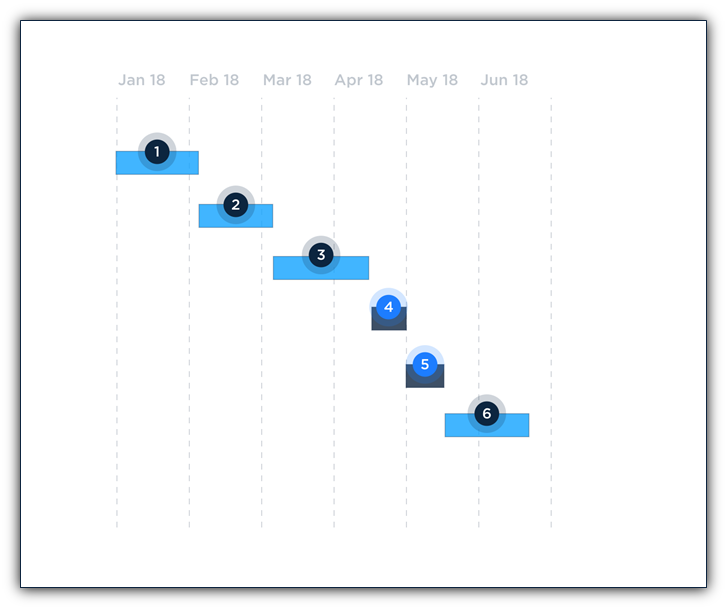
\includegraphics[scale=0.75]{media/gantt.png}
\caption{Research work plan}
\label{fig:gantt_chart}
\end{figure}

\section{Expected Results}
From this dissertation, it is expected that a proof-of-concept system with certain characteristics will emerge. The results will be analyzed to check if the system follows the parameters we are looking for.

For instance, it should be able to integrate information from various sources into a single place. This information should be available at any time, anywhere. It should be cryptographically secure, immutable, and easy and quick to share.

In the end, we need to analyze the results with the given metrics and ascertain whether there is a significant increase in performance and functionality that would justify using blockchain in a real supply chain.

%\todo{fcorreia: I'd expect to see here a list of contributions of your thesis. You do mention them, but a) I think they would be clearer to read as a list, b) you may be currently missing a few. I see at least 3 or 4, for example: a study of important design considerations for SCMSs, a study of important design considerations for blockchains, a prototype, an analysis of the benefits and liabilities of supporting a SCMS with a blockchain}

% pedro: I don't think a list is a good representation for the conclusion, especially when it is the ending of the document. And I don't know what other results to expect, I've written the ones we had discussed previously.




	%\chapter*{Epilogue}
\addcontentsline{toc}{chapter}{Epilogue}  

Lorem ipsum


    %\bookmarksetup{startatroot}
	%\phantomsection
	%\addcontentsline{toc}{part}{\appendixtocname}
	%\appendixpage
	%\appendix
		%\chapter{Statistical Analysis Methodology}
\label{chap:appendix-a}


    % Please add the following required packages to your document preamble:
% \usepackage{multirow}
% \usepackage[normalem]{ulem}
% \useunder{\uline}{\ul}{}
\begin{table}[]
    \centering
    \caption{Data analysis metrics used in the survey results analysis}
    \label{annex:metrics}
    \resizebox{\textwidth}{!}{
    \begin{tabular}{l|l|l|}
    \cline{2-3}
                                                                                                                                 & Metrics                                                                & Meaning                                                                                                                                                                                                                                                                                                                                                                                                                                                                                                                                                                                                                     \\ \hline
    \multicolumn{1}{|l|}{\multirow{3}{*}{\begin{tabular}[c]{@{}l@{}}Measures of\\ Central Tendency \\ or Location\end{tabular}}} & \textbf{Mean}                                                          & \begin{tabular}[c]{@{}l@{}}The mean represents the most probable value. In this\\ survey, with the use of scales with a lower and upper\\ bounds, the mean has the roles of representing the\\ average value of agreement, importance and other\\ measures.Normally, when the skewness of a distribution\\ is high, the meaning of the mean may get distorted by\\ the existence of outlier values. However, since the scales\\ have a low range, with a lower and upper bound on the\\ answer values, this is not much of a concern. Therefore,\\ even in cases of skewness, the mean can be a useful metric.\end{tabular} \\ \cline{2-3} 
    \multicolumn{1}{|l|}{}                                                                                                       & \textbf{Median}                                                        & \begin{tabular}[c]{@{}l@{}}Value of the 50\% percentile, for numerical answers. Half\\ the answers are above this value and half are below,\\ pointing to a central tendency around this value. This is\\ a good metric to use, especially in skewed distributions\\ where there are outliers in the collected values, since the\\ meaning of the mean may get slightly distorted by the\\ outlier values.\end{tabular}                                                                                                                                                                                                     \\ \cline{2-3} 
    \multicolumn{1}{|l|}{}                                                                                                       & \textbf{Mode}                                                          & \begin{tabular}[c]{@{}l@{}}Most frequent response. Though it represents the most\\ popular answers, by itself the metric means nothing else,\\ as there might be answers almost as popular or not.\end{tabular}                                                                                                                                                                                                                                                                                                                                                                                                             \\ \hline
    \multicolumn{1}{|l|}{\multirow{2}{*}{\begin{tabular}[c]{@{}l@{}}Measures of Spread,\\ Scale or Dispersion\end{tabular}}}     & \textbf{\begin{tabular}[c]{@{}l@{}}Standard \\ Deviation\end{tabular}} & \begin{tabular}[c]{@{}l@{}}Quantifies the variation within the data set, by showing\\ how much the distribution spreads to either sides of the\\ center. A high value for the standard deviation means\\ that there are a lot of values away from the mean, from\\ which can be concluded that there is not a general\\ consensus on a certain answers.A low value means that\\ there is consensus, since all the values of the data set are\\ bundled more closely together.\end{tabular}                                                                                                                                  \\ \cline{2-3} 
    \multicolumn{1}{|l|}{}                                                                                                       & \textbf{Range}                                                         & \begin{tabular}[c]{@{}l@{}}Difference between highest and lowest value of the data set.\\ Together with the standard deviation, indicates the dispersion\\ of the value of the answers. A range of 0 means that a\\ question had the same value for all responses, for instance.\\ This metric ignores the frequency with which each answer\\ was given, that is why it must be coupled with the standard\\ deviation to be relevant.\end{tabular}                                                                                                                                                                          \\ \hline
    \multicolumn{1}{|l|}{\begin{tabular}[c]{@{}l@{}}Measures of\\ Skewness and\\ Kurtosis\end{tabular}}                          & \textbf{Skew}                                                          & \begin{tabular}[c]{@{}l@{}}This metric indicates the lack of symmetry in a distribution,\\ where the results bunch up in one side of the distribution.\\ For instance, negative skewness values indicate a skew to\\ the left: the values bunch up at the right end of the distribution\\ and the left tail is long, indicating there are outliers in the lower\\ values.\end{tabular}                                                                                                                                                                                                                                      \\ \hline
    \end{tabular}
    }
    \end{table}
		%\chapter{Composer Model Class Diagram}
\label{chap:appendix-b}

\begin{figure}[h]
    \centering
    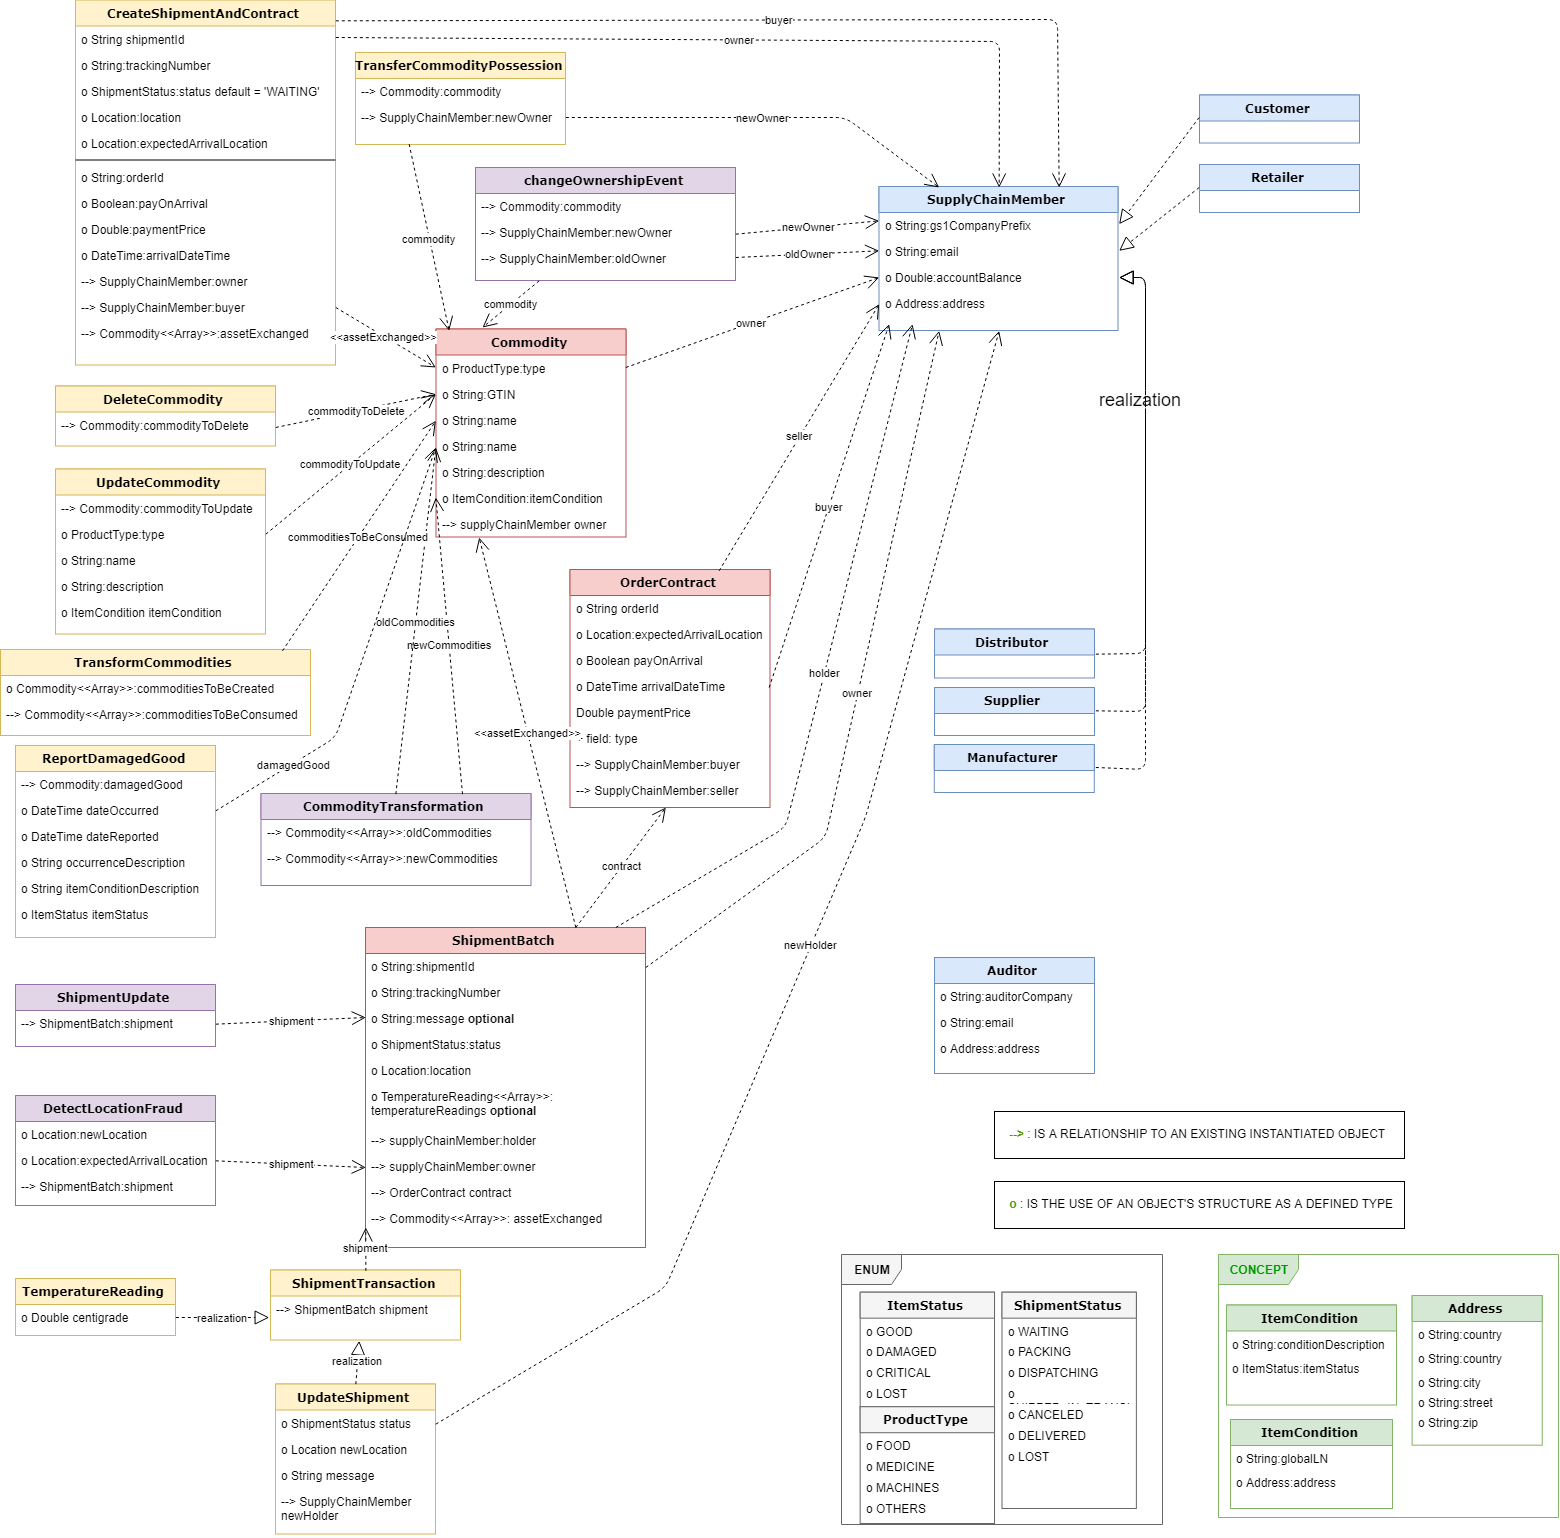
\includegraphics[scale=0.32]{media/full_class_diagram.png}
    \caption[Full class diagram for the designed Hyperledger Composer model]{Full class diagram for the designed Hyperledger Composer model}
    \label{fig:full_class_diagram}
\end{figure}



	% seealso index entries (must come after all other \index calls, so that they appear as the last subitems on index entries)
	%\index{knowledge!capture|seealso{expressiveness}}
	%\index{information|seealso{knowledge, capture}}

	
	\bookmarksetup{startatroot}
	\backmatter
		\cleardoublepage
		%\chapter{Publications}
\label{chap:publications}

Many of the materials in this thesis have appeared in the following publications.

\section*{Peer-reviewed Conference Papers}

Lorem ipsum.

\section*{Peer-reviewed Journal Papers}

Lorem ipsum.

\section*{Peer-reviewed Workshop Papers}

Lorem ipsum.

\section*{Peer-reviewed Posters}

Lorem ipsum.

\section*{Doctoral Symposiums}

Lorem ipsum.



		% Glossary
		%\cleardoublepage
		%\phantomsection
		%\begin{singlespace}
		%\begin{footnotesize}
		%\addcontentsline{toc}{chapter}{Nomenclature}
		%\markboth{Nomenclature}{Nomenclature}
		%\makenomenclature
		%% !TEX root = ../thesis.tex

\chapter*{Nomenclature}
\chaptermark{NOMENCLATURE}


\begin{flushleft}
\begin{tabular}{l p{0.8\linewidth}}
	ABB  & Abbreviation
\end{tabular}
\end{flushleft}

		%\printnomenclature[4.5cm]
		%\end{footnotesize}
		%\end{singlespace}

		% Bibliography / References
		\cleardoublepage
		\phantomsection
		\begin{singlespace}
		\begin{footnotesize}
		\addcontentsline{toc}{chapter}{References}
		\bibliographystyle{amsalpha}%{plainnat}
		\renewcommand{\bibname}{References}
		\bibliography{references}
		\end{footnotesize}
		\end{singlespace}
		\cleardoublepage
		\phantomsection
		\addcontentsline{toc}{chapter}{Index}
		\printindex
\end{document}
